\documentclass{report}
\usepackage[utf8]{inputenc}
\usepackage{amsmath, amsfonts, amsthm, graphicx, geometry, lipsum}
\usepackage{hyperref}
\usepackage{indentfirst}

\newtheorem{definition}{Definition}[section]
\newtheorem{lemma}{Lemma}[section]
\newtheorem{theorem}{Theorem}[section]
\newtheorem{corollary}{Corollary}[theorem]
\newtheorem{proposition}{Proposition}[theorem]


\newcommand{\N}{\mathbb{N}}
\newcommand{\Z}{\mathbb{Z}}
\newcommand{\R}{\mathbb{R}}

\title{MAT344 Introduction To Combinatorics\\
{\Large University of Toronto}}
\author{Haocheng Sun}
\date{Summer 2022}

\begin{document}
\maketitle

\tableofcontents

\chapter{Strings and Sets}

\section{Set}

\begin{definition}
    $[n]=\{0,1, \cdots ,n-1\}$, this notation will be helpful in computer science.
\end{definition}
e.g. $[1]=\{0\}$, $[3]=\{0,1,2\}$

\section{String}

\begin{definition}
    A \textbf{string} is an ordered list of objects. (Can have repetition)
\end{definition}
e.g. An english word is a string.

\begin{definition}
    Given a set $X$, 
    the map $s:[n] \rightarrow X$ is an \textbf{X-string} of length $n$. 
\end{definition}
The set $X$ can be viewed as the set of alphabets.

\begin{definition}
    A \textbf{binary string} is a string of 0's and 1's.
\end{definition}

\begin{definition}
    The \textbf{length} of a string is the number of objects in that string.
\end{definition}

\begin{theorem}
    Let $X$ be a collection of $n$ distinct objects. There are exactly $n^k$ many X-strings of length $k$.
\end{theorem}

\begin{proof}
    Note, an X-string of length k can be thought of as a function $s:[n] \rightarrow $X$. 
    A string $sS is uniquely determined by its values $s(i)$ for $i \in [k]$. 
    For each $i$, there are exactly $|X|=n$ possible values for $s(i)$ to be take. 
    It follows then there are exactly $n \times n \times \cdots \times n = n^k$ X-strings of length $k$. 
    (This is a \underline{counting argument})
\end{proof}

\section{Array}

\begin{definition}
    An \textbf{array} is an X-string $s$, where $s(i) \in X_i \subset X$.
\end{definition}
Arrays can be thought of as elements in the cartesian product $X_1 \times \cdots \times X_k$. 
An array is a string, but with restrctions.

\begin{theorem}
    There are exactly $|X_1| \times \cdots \times |X_k|$ many arrays in $X_1 \times \cdots \times X_k$.
\end{theorem}

\section{Permutation}

\begin{definition}
    Let $X$ be a collection of $n$ distinct objects. A \textbf{permutation} of $X$ is an X-string $s$ where no element is repeated.(i.e. $s$ is injecvtive when viewed as a function.)
\end{definition}
e.g. Let $X=\{a,b,c\}$, then a,b,c,ab,ac,,abc are all permutations of $X$.

\begin{definition}
    Given integers $n$ and $k$ with $n \geq k$. We use $P(n,k)$ to denote the number of permutations of $[n]$ of length $k$.
\end{definition}

\begin{definition}
    n factorial: $n!=n \times (n-1) \times \cdots \times 2 \times 1$.
\end{definition}

\begin{theorem}
    Given integers $n$ and $k$ with $n \geq k$, $$P(n,k)=\frac{n!}{(n-k)!}$$
\end{theorem}
\begin{proof}
    For a permutation of $[n]$ of length $k$, we have $n$ many choices for $s(0)$, $n-1$ remaining choices for $s(1)$,$\cdots$, $n-(k-1)$ remaining choices for $s(k-1)$. Hence, 
    $$P(n,k)=n \times \cdots \times n-(k-1)=\frac{n!}{(n-k)!}$$
\end{proof}

\section{Combinations}

\begin{definition}
    Given a set $X$, \textbf{a combination of size k} is a subset $A \subset X$ of size k of $[n]$. 
    We let ${n \choose k}$ denote the number of combinations of size k of $[n]$. 
    We read ${n \choose k}$ as n choose k.
\end{definition}

\begin{theorem}
    For positive integer $n$ and $k$ with $n \geq k$. 
    $${n \choose k} =\frac{P(n,k)}{k!}=\frac{n!}{(n-k)!k!}$$
\end{theorem}

\begin{proof}
    In order to create a permutation of $[n]$ of size k, it suffices to choose a combination $A \subset [n]$ of size k to be the range and permute it. 
    Thus, there are ${n \choose k} \times k!$ many ways to construct a [n]-permutations of size k. 
    Hoewever, we have defined $P(n,k)$ as the number of [n]-permutations of size k. 
    Hence $P(n,k)={n \choose k} \times k!$ i.e. ${n \choose k}=\frac{P(n,k)}{k!}$
\end{proof}
\chapter{Binomial Coefficients}

\section{Combinatorial Proof}

\textbf{Set-up}
\begin{itemize}
    \item Given an equation to prove. $LHS=RHS$
    \item Come up with some set of objects one of the sides (say $LHS$) is equivalent to in size.
    \item Come up with an alternative way to count the collection of objects that corresponds to the other side($RHS$).
    \item Conclude that you have counted the same set in two different ways to deduce $LHS=RHS$
\end{itemize}
Basically, it is proof by story telling.

\begin{theorem}
    $\forall n \in \N. 2^n=\sum_{k=0}^{n}{n \choose k}$
\end{theorem}
\begin{proof}
(The first combinatorial proof)
    \begin{itemize}
        \item Consider the collection of length $n$ binary strings. There are $2^n$ many such strings.
        \item Note, we can seperate strings in accordance with how many 1's the have. For $k \in \{0, \cdots ,n\}$, there are exactly ${n \choose k}$ many strings of length $n$ with k 1's. Therefore, there are $\sum_{k=0}^{n}{n \choose k}$ many binary strings.
        \item Thus, $2^n=\sum_{k=0}^{n}{n \choose k}$ as desired.
    \end{itemize}
\end{proof}
\begin{proof}
(The second combinatorial proof)
\begin{itemize}
    \item Suppose I am having a party and can invite any (or none) of my $n$ friends. There are $2^n$ many ways to do this, as there are $2^n$ many bsubsets from a collection of $n$ people.(for each people, choose him or not)
    \item Note, I can invite any number from $k=0, \cdots ,n$ of my friends. There are $2^n=\sum_{k=0}^{n}{n \choose k}$ many ways to choose k friends from n. Therefore, there are $\sum_{k=0}^{n}{n \choose k}$ many ways.
    \item Thus, $2^n=\sum_{k=0}^{n}{n \choose k}$ as desired.
\end{itemize}
\end{proof}

\section{Stars and Bars}
\begin{theorem}
    Let n, k be positive integers. There are ${n+(k-1) \choose k-1}$ integer solutions to the equatioin 
    $x_1 + \cdots + x_k=n$ with constraint $x_i \geq 0$ for all i.
\end{theorem}
\begin{proof}
    (This is not rigorous, I can only give you some intuition)\\
    Suppose there are n objects (represented by stars) to be placed into k bins. 
    The bins are distinguishable (say they are numbered 1 to k) but the n stars are not (so configurations are only distinguished by the number of stars present in each bin). 
    A configuration is thus represented by a k-tuple of non-negative integers, as in the statement of the theorem. Start by placing the stars in a line,
    we can place multiple bars between stars, before the first star and after the last star. 
    Since that any arrangement of stars and bars consists of a total of $n + k - 1$ objects, n of which are stars and $k-1$ of which are bars.
    We only need to choose $k - 1$ of the $n + k - 1$ positions to be bars (or, equivalently, choose n of the positions to be stars).
    Thus, there are ${n+(k-1) \choose k-1}$ arrangements.
\end{proof}

\begin{corollary}
    Let n, k be positive integers. There are ${n-1 \choose k-1}$ integer solutions to the equatioin 
    $x_1 + \cdots + x_k=n$ with constraint $x_i > 0$ for all i.
\end{corollary}
\begin{proof}
    The question is equivalent to find the number of solutions of $y_1 + \cdots + y_k=n-k$ with constraint $y_i \geq 0$ for all i.
    Then use the theorem above finish the proof.
\end{proof}

\section{Binomial Theorem}

\begin{theorem}
    $\forall x \in \R. (1+x)^n=\sum_{k=0}^{n}{n \choose k}x^k$
\end{theorem}

\begin{proof}
    We know that the function $f(x)=(1+x)^n$ is a polynomial, 
    so $f(x)=\sum_{k=0}^{n}c_kx^k$ for some $c_k \in \Z$. 
    Consider the derivative of $f(x)=(1+x)^n$, then the i-th derivative is $$f^{(i)}(x)=P(n,i)(1+x)^{n-i}$$ 
    Computed another way, we have $$f^{(i)}(x)=\sum_{k=1}^{n}c_kP(k,i)x^{k-i}$$
    Evaluating $f^{(i)}(0)$, we have $P(n,i)=c_iP(i,i)$. 
    Hence we get $$c_i=\frac{P(n,i)}{P(i,i)}=\frac{n!}{(n-i)!}\frac{(i-i)!}{i!}={n \choose i}$$ as desired.
\end{proof}

\begin{theorem}[Full Binomial Theorem]
    $\forall x \in \R. (x+y)^n=\sum_{k=0}^{n}{n \choose k}x^ky^{n-k}$
\end{theorem}
\begin{proof}
    It is true when $y=0$, so suppose $y \neq 0$. 
    Note $(x+y)^n=y^n(1+\frac{x}{y})^n$ ,so set $z=\frac{x}{y}$. 
    finally we have 
    \begin{equation}
        \begin{split}
            y^n(1+\frac{x}{y}) &= y^n \sum_{k=0}^{n}{n \choose k}z^k\\
            &= y^n \sum_{k=0}^{n}{n \choose k}x^ky^{-k}\\
            &= \sum_{k=0}^n{n \choose k}x^ky^{n-k}
        \end{split}
    \end{equation}
\end{proof}

\section{Lattice and Catalan number}

\begin{definition}
    A \textbf{lattice} is a set of the form $[n+1] \times [m+1]$. 
    We call a lattice of this form \textbf{an n by m lattice}. 
    The point $(0,0) \in [n+1]\times [m+1]$ is called the  \textbf{origin}.
\end{definition}

\begin{definition}
    A \textbf{lattice path} is a swquence $\{(a_0,b_0),(a_1,b_1), \cdots ,(a_{n+m},b_{n+m})\}$ 
    that satisfies the property that:\\
    \begin{itemize}
        \item $(a_0,b_0)=(0,0)$
        \item $(a_{n+m},b_{n+m})=(n,m)$
        \item $(m_{i+1},n_{i+1})=(m_{i+1},n_i)$ or $(m_{i+1},n_{i+1})=(m_{i},n_{i+1})$
    \end{itemize}
\end{definition}

\begin{theorem}
    Given an n by m lattice, there are ${n+m \choose n}$ many ways to walk from the origin to $(n,m)$.
\end{theorem}
\begin{proof}\
    \begin{itemize}
        \item Nottice that a lattice path is codified by an length $n+m$ sequence from $\{U,R\}$ with n many R's(U means up and R means right)
        \item To see this, notice the following reversible process to get a walk from a sequence and vice versa.
        \item Given a lattice path $P=\{(a_o.b_0),(a_1,b_1), \cdots ,(a_{n+m},b_{n+m})\}$, assign to it a sequence $s:[n+m] \rightarrow \{U,R\}$ where $s(i)=U$ iff $b_{i+1}=b_i+1$.
        \item To reverse this, given a sequence $s:[n+m] \rightarrow \{U,R\}$, assign to it a lattice path $P=\{(a_o.b_0),(a_1,b_1), \cdots ,(a_{n+m},b_{n+m})\}$ where $b_{i+1}=b_i+1$ when $s(i)=U$ or alternatively, $a_{i+1}=a_i+1$ when $s(i)=R$
    \end{itemize}
\end{proof}

\begin{definition}
    We define the \textbf{Catalan number} $C(n)$ to be the number of lattice paths from $(0,0)$ to $(n,n)$ that stay below the line $y=x$.
\end{definition}

\begin{theorem}
    The catalan number can be explicitly computed,
    $$C(n)=\frac{1}{n+1}{2n \choose n}$$
\end{theorem}
\begin{proof}
(proof1, Total - Above Diagonal)
\begin{itemize}
    \item Total= ${2n \choose n}= \frac{(2n)!}{n!n!}$
    \item Above= ${2n \choose n+1}= \frac{(2n)!}{(n+1)!(n-1)!}$ (this part is very tricky, I will not give details)
    \item $C(n)={2n \choose n}-{2n \choose n+1}=\frac{1}{n+1}{2n \choose n}$
\end{itemize}
\end{proof}
\begin{proof}
(proof2, Find the recurrence relation)\\
Let $k \in \{1, \cdots ,n\}$ be arbitrary, consider the spot $(k,k)$.\\
Let $S_k$ denotes the set of paths which first intersect the line $y=x$ at point $(k,k)$.\\
For $k=0$ the only path is stay at the origin, hence $c_0=|S_0|=1$.\\
For $k \in \{1, \cdots ,n\}$, can check that $|S_k|=c_{k-1} \cdot c_{n+1-k}$\\
Since $\{S_0, \cdots ,S_k\}$ forms a partition of $S_{n+1}$, hence we get the following recurrence
\begin{equation}
    \begin{cases}
        c_0=1\\
        c_{n+1}=\sum_{i=0}^{n}c_ic_{n-i}
    \end{cases}
\end{equation}
We can check the example of \ref{cnr} to finish the proof.
\end{proof}
\noindent Example: How many ways can we parenthesize the string abcdef?
\chapter{Induction and Pigeon hole principle}

\section{Well-ordering}
As usual, before we talk about well-ordering, we need to introduce the concept of relations and partial order. But since we are familiar with these concepts, this course will skip these concepts here and focus using graphs to study partial orders in the future.
\begin{definition}
    An ordered set $(S,<)$ is caleed \textbf{well ordered} if every non-empty subset $X \subset S$ has a smallese element.
\end{definition}
e.g. The natural numbers $\N$ with the usual $<$.

\section{Intoduction to Recerrence}
\begin{definition}
    A \textbf{recurrence relation} is any sequence whose value depends on its previous values. 
    A recurrence more broadly refers to any self referential statement.
\end{definition}

\begin{theorem}
    $\forall n \in \N. \forall k \in \N. {n \choose k}={n-1 \choose k-1}+{n-1 \choose k}$
\end{theorem}
\begin{proof}
    (use a combinatorial proof)
    \begin{itemize}
        \item Suppose I want to hire people from a group of m. Suppose one of the people is named Ken.
        \item The LHS counts the number of ways I can hire k people.
        \item Alternatively, I can split into two cases, one when I hire Ken and one where I do not.
    \end{itemize}
\end{proof}

\section{Induction}

\begin{theorem}[Simple inductin]
    For every $k \in \N$. Let $P(k)$ be a statement. Suppose we can show that for every k
    \begin{itemize}
        \item $P(1)$ is true. (base case)
        \item $P(k) \Rightarrow P(k+1)$. (inductive step)
    \end{itemize}
    It follows that for all $k \in \N$, $P(k)$ is true.
\end{theorem}

\begin{theorem}[Strong Induction]
    Let $P(n)$ be a collection of statements indexed bt $n \in \N$. Given
    \begin{itemize}
        \item $P(1)$ is true.
        \item $\forall n \in \N.[(\forall k \in \N. k<n \Rightarrow P(k)) \Rightarrow P(n)]$
    \end{itemize}
    Then $\forall n \in \N. P(n)$
\end{theorem}
\textbf{Remark}
\begin{itemize}
    \item The primary distinction between choosing induction and strong induction is that simple induction only uses one piece of past information, strong induction uses all past information.
    \item We prove simple induction and strong induction are equivalent in CSC240.
\end{itemize}


\section{Pigeon Hole Principle}
As it is a very usefull theorem from our elementary school math to the theory of computation, 
we will use a whole section to talk about this theorem.\\
\begin{theorem}[Pigeon hole principle 1]
    Let $X$ be a set of n objects. 
    Suppose $\{X_1, \cdots ,X_k\}$ form a partition of $X$. 
    If $k<n$, then $\exists i \in \{1, \cdots ,k\}. |X_i| \geq 2$
\end{theorem}
\begin{proof}
    (By way of contradiction)
    Suppose that for all $i \in \{1, \cdots ,k\}. |X_i|=1$. 
    Since $\{X_1, \cdots ,X_k\}$ is a partition, then $n=|X|=\sum_{i=1}^k|X_i|=k$. Contradiction as $k<n$.
\end{proof}

\begin{theorem}[Pigeon hole principle 2]
    Let $X$ be a set of n objects. Let $s:X \rightarrow \{1, \cdots ,k\}$. 
    If $k<n$, then $s$ cannot be injective. i.e. there are distinct $x,y \in X$ such that $s(x)=s(y)$.
\end{theorem}
\begin{proof}
    For $i \in \{1, \cdots ,k\}$, set $X_i=\{x \in X: s(x)=i\}$. 
    $X_i$ are disjoint and $\bigcup_{i=1}^kX_i=X$.
    Assume $s$ is injective. By definition, $\forall i \in \{1, \cdots ,k\}. \exists ! x \in X. s(x)=i$
    Therefore, we have a contradiction that $\bigcup_{i=1}^k|X_i|=k < n=|X|$
\end{proof}

\begin{theorem}[Generalized PHP]
    Fix $k,m \in \N$, sets $X$ and $Y$ with $|X|=km+1$ and $|Y|=m$, 
    and a function $f:X \rightarrow Y$. Then there is an element $y \in Y$ with at least $k+1$ preimages. 
    That is to say, there exist $x_1, \cdots ,x_k,x_{k+1} \in X$ distinct elements such that $f(x_1)=f(x_2)= \cdots =f(x_k)=f(x_{k+1})$.
\end{theorem}
\begin{proof}
    We want to show that $$\exists y \in Y. |f^{-1}(y)| \geq k+1$$
    So we assume the negation that $$\forall y \in Y. |f^{-1}(y)| \leq k$$
    Since we do not know whether the function $f$ is surjective. So explicitly: $$\forall y \in f(X). |f^{-1}(y)| \leq k$$
    Since $|Y|=m$, then we have $|f(X)| \leq m$. Since $X \rightarrow f(X)$ is a surjection. Then $\{X_y\}_{y \in f(X)}$ is a partition of $X$. 
    Hence $$|X|=\sum_{y \in f(X)}|X_y| \leq m \times k=mk$$
    But we already have $$|X|=km+1 >mk$$
    This is a contradiction
\end{proof}

\noindent \textbf{Example}:
\begin{enumerate}
    \item Let $X$ be a set of 5 odd integers.\\
    There is a disjoint pair $a,b \in X$ such that $a-b$ is divisible by 8.
    \item For every $n \in \N$, there is a number who's decimal expansion only consists of 5's and 0's that is divisible by $n$.
    \begin{itemize}
        \item $n=1$ we have 5
        \item $n=2$ we have 50
        \item $n=3$ we have 555
        \item $n=4$ we have 500
        \item $n=5$ we have 5
    \end{itemize}
    Proof of the claim:\\
    Fix $n \in \N$, consider $X=\{\sum_{i=0}^k5 \cdot 10^i | k \in \{0, \cdots,n\}\}$
    \begin{itemize}
        \item $k=0$ we have $5 \cdot 10^0=5$
        \item $k=1$ we have $5 \cdot 10^0 + 5 \cdot 10^1=55$
        \item $k=2$ we have $5 \cdot 10^0 + 5 \cdot 10^1 + 5 \cdot 10^2=555$
    \end{itemize}
    Consider the following partition $X_i=\{q \in X | q \equiv i \text{ mod } n\}$. 
    This partition $X$ into $n$ pieces. 
    By Pigeon hole principle, $$\exists i \in \{0,\cdots,n-1\}. |X_i| \geq 2$$
    We take the biggest one and the smallest one in that set, take their difference, 
    that thing is going to be divisible by n because they are in the same equivalent class.
\end{enumerate}
\chapter{Inclusion and Exclusion}


\section{principle of Inclusion-Exclusion}

\begin{definition}
    Let $S$ be a set. Fix a collection $A_i \subset S$ indexed by $i \in \{1,\cdots,n\}$. 
    Given $I \subset \{1,\cdots,n\}$, we let $A_I= \bigcap_{i \in I}A_i$. We set $A_{\emptyset}=S$.
\end{definition}
\textbf{Remark}:
\begin{itemize}
    \item $S$ is the set of all things.
    \item $A_i$ is a set of elements in $S$ which are restricted by property indexed by $i$.
    \item $A_I$ is the set of elements which are restricted by properties $I \subset \{1,\cdots,n\}$.
    \item $A_{\emptyset}$ restricted by no property, hence is $S$.
    \item This will help us simplify our notation.
\end{itemize}

\textbf{Example}:Let $S=\{1,2,\cdots,20\}$ and let 
$$A_1=\{x \in S: x \text{ is divisible by } 2\}$$
$$A_2=\{x \in S: x \text{ is divisible by } 3\}$$
$$A_3=\{x \in S: x \text{ is divisible by } 4\}$$
\begin{itemize}
    \item $A_{\emptyset}=S=\{1,2,\cdots,20\}$
    \item $A_{\{1,2\}}=\{6,12,18\}$ these are elements in $S$ that are divisible by 6
    \item $A_{\{1,3\}}=\{4,8,12,16,20\}$ these are elements in $S$ that are divisible by 4
    \item $A_{\{1,2,3\}}=\{12\}$ these are elements in $S$ that are divisible by 12
\end{itemize}

\begin{theorem}[Basic rule]
    $$|A \cup B|=|A|+|B|-|A \cap B|$$
\end{theorem}
\begin{proof}
    We can use some basic set theory knowledge to prove this.
\end{proof}

\begin{theorem}[MIT notation]
    $$|\cup_{i=1}^nA_i|= \sum_{\emptyset \neq I \subset \{1,\cdots,n\}}(-1)^{|I|+1}|\cap_{i \in I}A_i|$$
\end{theorem}
\begin{proof}
    Induction on $n \in \N$\\
    Base case: $$|A_1|=(-1)^2|A_1|=\sum_{\emptyset \neq I \subset \{1\}}|\cap_{i \in I}A_i|$$
    Inductive step: Assume the theorem is true for $n$. Let $A_1,\cdots,A_n,A_{n+1}$ be subsets of $S$.
    \begin{equation}
        \begin{split}
            |\cup_{i=1}^{n+1}A_i| =& |\cup_{i=1}^nA_i|+|A_{n+1}|-|(\cup_{i=1}^nA_i)\cap A_{n+1}| \text{ (by the basic rule)}\\
            =& |\cup_{i=1}^nA_i|+|A_{n+1}| -|(A_1\cap A_{n+1})\cup \cdots \cup(A_n\cap A_{n+1})|\\
            =& \sum_{\emptyset \neq I \subset \{1,\cdots,n\}}(-1)^{|I|+1}|\cap_{i \in I}A_i| + |A_{n+1}|- \sum_{\emptyset \neq I \subset \{1,\cdots,n\}}(-1)^{|I|+1}|\cap_{i \in I}(A_i \cap A_{n+1})| \text{ (by I.H.)}\\
            =& \sum_{\emptyset \neq I \subset \{1,\cdots,n\}}(-1)^{|I|+1}|\cap_{i \in I}A_i| - (-1)^{|\{n+1\}|} -\sum_{J \subset \{1,\cdots,n+!\}}(-1)^{|J|}|\cap_{i \in J}A_i|\\
            & \text{ where } J \in \{I \cup \{n+1\}: \emptyset \neq I \subset \{1,\cdots,n\}\}\\
            =& \sum_{P \subset \{1,\cdots,n\}}(-1)^{|P|+1}|\cap_{i \in P}A_i| + \sum_{Q \subset \{1,\cdots,n+1\}}(-1)^{|Q|+1}|\cap_{i \in Q}A_i|\\
            & \text{ where } P \in \{I: \empty \neq I \subset \{1,\cdots,n\}\}, Q \in \{I\cup \{n+1\}: I \subset \{1,\cdots,n\}\}\\
            & \text{ Note that the first part has no $A_{n+1}$ and the second part has $A_{n+1}$}\\
            =& \sum_{\emptyset \neq T \subset \{1,\cdots,n+1\}}(-1)^{|T|+1}|\cap_{i \in T}A_i|
        \end{split}
    \end{equation}
    This is totally my proof, I think it is intuitive and direct.
\end{proof}

\begin{theorem}[Our notation]
    Let $S$ be a set. Fix a collection $A_i \subset S$ indexes by $i \in \{1,\cdots,n\}$. 
    Then we have $$|S \setminus \cup_{i=1}^nA_i|= \sum_{I \subset \{1,\cdots,n\}}(-1)^{|I|}|A_I|$$
\end{theorem}
\begin{proof}
    By induction on $n$.\\
    Base case:
    \begin{equation}
        \begin{split}
            \sum_{I \subset \{1\}}(-1)^{|I|}|A_I| &= (-1)^0|A_{\emptyset}| + (-1)^1|A_{\{1\}}|\\
            &= |S| - |A_{1}|\\
            &= |S \setminus A_1|
        \end{split}
    \end{equation}
    Inductive step: Assume the theorem is true for $n$. Let $A_1,\cdots,A_n,A_{n+1}$ be subsets of $S$. 
    Let $B_i=A_i \cap A_{n+1}$ for $i \in \{1,\cdots,n\}$ (note $B_{\emptyset}=A_{\emptyset}\cap A_{n+1}=A_{n+1}$)
    \begin{equation}
        \begin{split}
            \sum_{I \subset \{1,\cdots,n+1\}}(-1)^{|I|}|A_I| &= \sum_{I \subset \{1,\cdots,n\}}(-1)^{|I|}|A_I| + \sum_{I \subset \{1,\cdots,n\}}(-1)^{|I|+1}|A_{I \cup \{n+1\}}|\\
            &= |S \setminus \cup_{i=1}^nA_i| - \sum_{I \subset \{1,\cdots,n+1\}}(-1)^{|I|}|B_I|\\
            &= |S \setminus \cup_{i=1}^nA_i| -|B_{\emptyset} \setminus \cup_{i=1}^nB_i|\\
            &= |S \setminus \cup_{i=1}^nA_i| -|A_{n+1}\setminus \cup_{i=1}^n(A_i \cap A_{n+1})|\\
            &= |S \setminus \cup_{i=1}^nA_i| -|A_{n+1}\setminus \cup_{i=1}^nA_i|\\
            &= |(S \setminus \cup_{i=1}^nA_i) \setminus (A_{n+1} \setminus \cup_{i=1}^nA_i)|\\
            &= |(S \cup (\cup_{i=1}^nA_i)) \setminus ((\cup_{i=1}^nA_i)\cup A_{n+1})|\\
            &= |S \cup (\cup_{i=1}^{n+1}A_i)|
        \end{split}
    \end{equation}
\end{proof}
\textbf{Remark}:
\begin{itemize}
    \item We will use our notation during the course.
    \item This theorem transform counting unions to counting intersections.
    \item Intersections are easier to count since no overlap.
\end{itemize}

\noindent \textbf{Questions}:
\begin{enumerate}
    \item Compute the number of integer solutions to the equation $x_1+x_2+x_3+x_4=100$ with $x_1,x_2 \leq 10$ and $x_i \geq 0$ for all $i \in \{1,2,3,4\}$.
    \item A wizard has 5 friends. During a long wizards' conference. They met any given friend at dinner 10 times, any pair of friends 5 times, 
    any given threesome of friends 3 times, any given foursome 2 times, and all 5 friends together once. 
    The wizard ate along 6 times. Determine how many days the wizards' conference lasted.
\end{enumerate}

\noindent \textbf{Answer}:
\begin{enumerate}
    \item Let $S$ be the set of sokutions with $x_i \geq 0$ for all $i \in \{1,2,3,4\}$.\\
    Let $A_1$ be the set of solutions with $x_1 \geq 11$ and $x_i \geq 0$.\\
    Let $A_2$ be the set of solutions with $x_2 \geq 11$ and $x_i \geq 0$.\\
    We want to count $|S \setminus (A_1 \cup A_2)|$
    \begin{equation}
        \begin{split}
            |S \setminus (A_1 \cup A_2)| &= |S| -|A_1| -|A_2| + |A_1 \cap A_2|\\
            &= {100+3 \choose 3} -{89+3 \choose 3}-{89+3 \choose 3}+{78+3 \choose 3}
        \end{split}
    \end{equation}
    \item Let $S$ be the set of all days. Let $\{1,2,3,4,5\}$ denotes the set of all friends.\\
    Let $A_i=\{\text{days when the wizards met person i}\}$ for $i \in \{1,2,3,4,5\}$.\\
    From the question, we have 
    $$|A_1|=|A_2|=\cdots=|A_5|=10$$
    $$|A_{\{1,2\}}|=|A_{\{1,3\}}|=\cdots=|A_{\{4,5\}}|=5$$
    $$\forall I \subset \{1,2,3,4,5\} \text{ with } |I|=3. |A_I|=3$$
    $$\forall I \subset \{1,2,3,4,5\} \text{ with } |I|=4. |A_I|=2$$
    $$\forall I \subset \{1,2,3,4,5\} \text{ with } |I|=5. |A_I|=1$$
    $$|S \setminus \cup_{i=1}^5A_i|= |\{\text{days the wizard eats along}\}|=6$$
    By our theorem we have:
    \begin{equation}
        \begin{split}
            \sum_{I \subset \{1,\cdots,5\}}(-1)^{|I|}|A_I| &= |S| + \sum_{\emptyset \neq I \subset \{1,\cdots,n\}}(-1)^{|I|}|A_I|=6\\
            |S| &= 6 - \sum_{\emptyset \neq I \subset \{1,\cdots,n\}}(-1)^{|I|}|A_I|
        \end{split}
    \end{equation}
\end{enumerate}



\section{Counting Surjections}

\begin{definition}
    A function $f: X \longrightarrow Y$ is called a \textbf{surjection} if 
    $$\forall y \in Y. \exists x \in X. f(x)=y$$
\end{definition}

\begin{theorem}[Counting Surjections]
    Let $S(n,m)$ denotes the number of surjections $f:[n] \longrightarrow [m]$, 
    then $$S(n,m)=\sum_{k=0}^m(-1)^k{m \choose k}(m-k)^n$$
\end{theorem}
\begin{proof}
    We will use the inclusion-exclusion principle. Let $S$ be the set of all functions from $[n]$ to $[m]$. 
    For each $i \in [m]$, let $A_i=\{f: \forall x \in [n].f(x) \neq i\}$. Note, $S \setminus \cup_{i \in [n]}A_i$ is the set of surjective functions. 
    Note that for any $I \subset [m]$ of size $k$, $|A_I|=(m-k)^n$. This is because $A_I=\cap_{i \in I}A_i$ is the set of all functions that miss all of $I$.
    \begin{equation}
        \begin{split}
            S(n,m) &= |S \setminus \cup_{i \in [m]}A_i|\\
            &= \sum_{I \subset [m]}(-1)^{|I|}|A_I|\\
            &= \sum_{I \subset [m] \text{ with } |I|=0}(-1)^{|I|}|A_I| + \sum_{I \subset [m] \text{ with } |I|=1}(-1)^{|I|}|A_I| + \cdots + \sum_{I \subset [m] \text{ with } |I|=m}(-1)^{|I|}|A_I|\\
            &= \sum_{k=0}^m \sum_{I \subset [m] \text{ with } |I|=k}(-1)^{k}|A_I|\\
            &= \sum_{k=0}^m \sum_{I \subset [m] \text{ with } |I|=k}(-1)^{k}(m-k)^n\\
            &= \sum_{k=0}^m {m \choose k}(-1)^{k}|A_I|\\
        \end{split}
    \end{equation}
\end{proof}

\noindent \textbf{Question}: A teacher has 10 books(all different) that she wants to distribute to John, Paul, Ringo, George, 
ensuring that each of them gets at least one book. In how many ways can she do this? 
Compare this answer to when the books are not distinct.

\noindent \textbf{Answer}:
\begin{itemize}
    \item For different books, lets label them as $\{1,\cdots,10\}$
    $$S=\{f| f:\{1,\cdots,10\} \longrightarrow \{J,P,R,G\}\}$$
    $$|S|=S(10,4)$$
    \item For not different books, we use stars and bars:
    \begin{equation}
        \begin{cases}
            x_1+x_2+x_3+x_4 =10\\
            x_i \geq1 \text{ for all } i
        \end{cases}
    \end{equation}
    This is equivalent to:
    \begin{equation}
        \begin{cases}
            y_1+y_2+y_3+y_4=6\\
            y_i \geq 0 \text{ for all } i
        \end{cases}
    \end{equation}
\end{itemize}



\section{Counting Derangements}

\begin{definition}
    A \textbf{derangement} is a permutation $s:[N] \longrightarrow [N]$ that has no fixed points. 
    i.e. with the property that $\forall i \in[n]. s(i) \neq i$. 
    We denote the number of Derangements with $d_n$
\end{definition}

\begin{theorem}[Counting Derangements]
    $$d_n=\sum_{k=0}^n(-1)^k{n \choose k}(n-k)!=n!\sum_{k=0}^n\frac{(-1)^k}{k!}$$
\end{theorem}
\begin{proof}
    For $i \in[n]$. Let $A_i$ be the set of permutations $s$ that satisfy $s(i)=i$. 
    Let $S$ be the set of permutations of $[n]$. 
    Note that $S \setminus \cup_{i \in [n]}A_i$ is the set of all Derangements. 
    Note that for any $I \subset [n]$ of size $k$, $|A_I|=(n-k)!$. 
    Similarly to counting surjections, we have
    \begin{equation}
        \begin{split}
            d_n &= \sum_{I \subset [n]}(-1)^{|I|}|A_I|\\
        &= \sum_{k=0}^n(-1)^k{n \choose k}(n-k)!\\
        &= \sum_{k=0}^n(-1)^k \frac{n!}{k!(n-k)!}(n-k)!\\
        &= n!\sum_{k=0}^n\frac{(-1)^k}{k!}
        \end{split}
    \end{equation}
\end{proof}
\textbf{Remark}:
\begin{itemize}
    \item Consider something interesting:
    $$\frac{\text{number of derangements}}{\text{number of permutations}}=\frac{d_n}{n!}=\sum_{k=0}^n\frac{(-1)^k}{k!}$$
    We notice that this is a probability, so it is between 0 and 1. What happens when $n$ gets bigger and bigger?
    $$\sum_{k=0}^{\infty}\frac{(-1)^k}{k!}=\frac{1}{e}$$
    \item We have alternative ways to get $d_n$.
    \begin{itemize}
        \item We can use a combinatorial proof to show for $n \geq 2$, $$d_n=(n-1)(d_{n-2}+d_{n-1})$$
        \item We can do by algebra to show for $n \geq 2$, $$d_n=n \cdot d_{n-1}+(-1)^n$$
    \end{itemize}
\end{itemize}


\section{Euler's Totient Function}

\begin{definition}
    Given two integers $n,m$, we call the \textbf{greatest common divisor (GCD)} of $n$ and $m$ the largest integer which divides both $n$ and $m$. 
    We sometimes call this quantity $gcd(n,m)$.
\end{definition}

\begin{definition}
    We say two integers $n,m$ are \textbf{relatively prime} if $gcd(n,m)=1$.
\end{definition}


\begin{definition}[Euler's Totient Function]
    For $n \in \N$, define:
    $$\phi(n)=|\{m \in \{1,\cdots,n\}: gcd(m,n)=1\}|$$
\end{definition}
\textbf{Remark}:
\begin{itemize}
    \item This function is of deep interest in number theory and group theory.
\end{itemize}


\begin{lemma}
    Let $n \geq 2$ be an integer. Let $p_1,\cdots,p_k$ be a collection of distinct primes that divide $n$. 
    There are $\frac{n}{p_1\times \cdots \times p_k}$ integers in $\{1,\cdots,n\}$.
\end{lemma}
\begin{proof}
    Suppose $m \in \N$ and $m$ is divisible by all the $p_1,\cdots,p_k$. 
    It follows then that $m=p_1 \times \cdots \times p_k\times \alpha$ for some $\alpha \in \N$. So
    $$p_1 \times \cdots \times p_k \leq p_1 \times \cdots \times p_k \times \alpha \leq n$$
    This implies that $$1 \leq \alpha \leq \frac{n}{p_1 \times \cdots \times p_k}$$
\end{proof}

\begin{lemma}
    (We will use this lemma to prove the following theorem)
    $$\prod_{i=1}^k(1-x_i)=\sum_{I \subset \{1,\cdots,k\}} \prod_{i \in I}(-x_i)$$
\end{lemma}
\begin{proof}
    Induction on $k$.\\
    Base case: $k=1$ 
    \begin{equation}
        \begin{split}
            \sum_{I \subset \{1\}} \prod_{i \in I}(-x_i) &= \prod_{i \in \emptyset}(-x_i)+ \prod_{i \in \{1\}}(-x_i)\\
            &= 1 + (-x_1) \text{ (the empty product is 1)}\\
            &= \prod_{i=1}^1(1-x_i)
        \end{split}
    \end{equation}
    Inductive step:
    \begin{equation}
        \begin{split}
            \prod_{i=1}^{k+1}(1-x_i) =& (\prod_{i=1}^{k}(1-x_i))\times (1-x_{k+1})\\
            =& \sum_{I \subset \{1,\cdots,k\}} \prod_{i \in I}(-x_i) - x_{k+1} \times \sum_{I \subset \{1,\cdots,k\}} \prod_{i \in I}(-x_i)\\
            =& \sum_{P \subset \{1,\cdots,k+1\}} \prod_{i \in P}(-x_i) + \sum_{Q \subset \{1,\cdots,k+1\}} \prod_{i \in Q}(-x_i)\\
            & \text{ where } P \in \{I: I \subset \{1,\cdots,k\}\}, Q \in \{I \cup\{k+1\}: I \subset \{1,\cdots,k\}\}\\
            =& \sum_{L \subset \{1,\cdots,k+1\}} \prod_{i \in L}(-x_i)
        \end{split}
    \end{equation}
\end{proof}


\begin{theorem}[Compute $\phi(n)$]
    For all $n \geq 2$. Assume $p_1, \cdots,p_k$ are all prime factors of $n$. Then
    $$\phi(n)=n \times \prod_{i=1}^k \frac{p_i-1}{p_i}$$
\end{theorem}
\begin{proof}
    For each $i \in \{1,\cdots,k\}$. Let $A_i$ be the set of integers in $\{1,\cdots,n\}$ that are divisible by $p_i$. 
    Note, $\{1,\cdots,n\}\setminus \cup_{i=1}^kA_i$ is the set of positive integers $\leq n$ that are relatively prime with $n$. 
    By our lemma, for any $I \subset \{1,\cdots,n\}. |A_I|=|\cap_{i \in I}A_i|$. 
    Fix $i$, for $p_i$, by the lemma, there are $\frac{n}{p_i}$ numbers that are divisible by $p_i$ and $\leq n$. 
    This shows $$|A_I|=\prod_{i \in I}\frac{n}{p_i}=n \cdot \prod_{i \in I}\frac{1}{p_i}$$
    By definition of $\phi(n)$,
    \begin{equation}
        \begin{split}
            \phi(n) &= |\{1,\cdots,n\}\setminus \cup_{i=1}^kA_i|\\
            &= \sum_{I \subset \{1,\cdots,k\}}(-1)^{|I|}|A_I| \text{ (by inclusion-exclusion)}\\
            &= \sum_{I \subset \{1,\cdots,k\}}(-1)^{|I|}n \cdot \prod_{i \in I}\frac{1}{p_i}\\
            &= n \cdot \sum_{I \subset \{1,\cdots,k\}}(-1)^{|I|} \cdot \prod_{i \in I}\frac{1}{p_i}\\
            &= n \cdot \sum_{I \subset \{1,\cdots,k\}}\cdot \prod_{i \in I}\frac{(-1)}{p_i}\\
            &= n \cdot \sum_{i \in \{1,\cdots,k\}}(1-\frac{1}{p_i}) \text{ (by the lemma above)}\\
            &= n \times \prod_{i=1}^k \frac{p_i-1}{p_i}
        \end{split}
    \end{equation}
\end{proof}
\chapter{Graph Theory}

\section{Graph Basics}

\begin{definition}
    A \textbf{graph} is a pair $(V,E)$ where $V$ is a finite set, called the \textbf{vertex set}, it's members are called \textbf{vertices}. 
    and $E$ is a collection of subsets of $V$ of size 2. $E$ is called \textbf{edge set}, it's members are called \textbf{edges}.
\end{definition}
\textbf{Remark}:
\begin{itemize}
    \item We generally reserve the name $G$ for graphs.
    \item The textbook likes to write $xy$ or $yx$ to denote an edge. I like more cumbersome notation $\{x,y\}$.
    \item If $x,y \in V$ and $\{x,y\} \in E$, we say $x$ and $y$ are \textbf{adjacent}.
    \item We will not prove things with graphs, but we will think about graphs.
    $$\text{\underline{Think geometrically but proof rigidly.}}$$
    Recall how we proved the pumping lemma in theory of computation.
\end{itemize}


\begin{definition}
    For $n \geq 1$, we let $\mathbf{K_n}$ denote the \textbf{complete graph} $([n],E)$ where $$E=\{e \subset [n]: |e|=2\}$$
\end{definition}
\begin{figure}[ht]
    \centering
    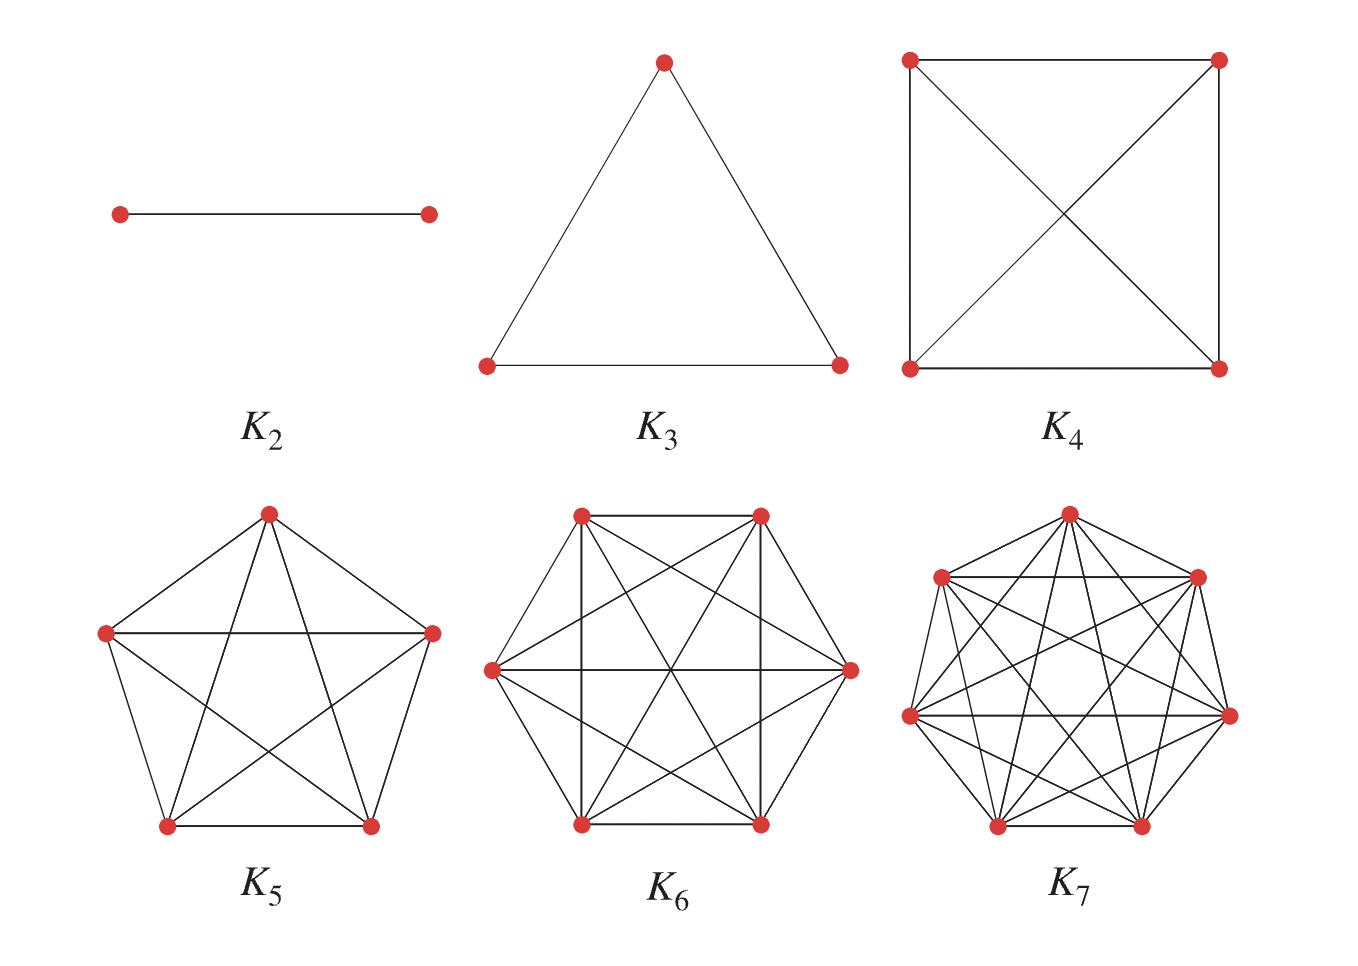
\includegraphics[scale=0.4]{Images/cg.png}
    \caption{A picture of complete graphs}
\end{figure}

\begin{definition}
    For $n \geq 1$, we let $\mathbf{P_n}$ denote the \textbf{path graph}(sometimes called the \textbf{linear graph}) $([n],E)$ where $$E=\{\{i,i+1\} \subset [n]: i \in [n]\}$$
\end{definition}
\begin{figure}[ht]
    \centering
    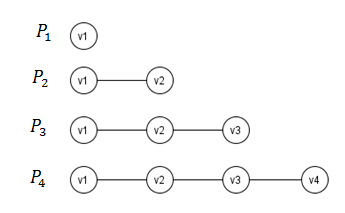
\includegraphics[scale=0.45]{Images/Figure-3Paths-Definition314-The-Cycle-is-a-path-graph-that-its-initial-vertex.jpg}
    \caption{A picture of path graphs}
\end{figure}

\begin{definition}
    For $n \geq 3$, we let $\mathbf{C_n}$ denote the \textbf{cycle graph} $([n],E)$ where $$E=\{\{0,1\},\{1,2\},\cdots,\{n-1,0\}\}$$
\end{definition}
\begin{figure}[ht]
    \centering
    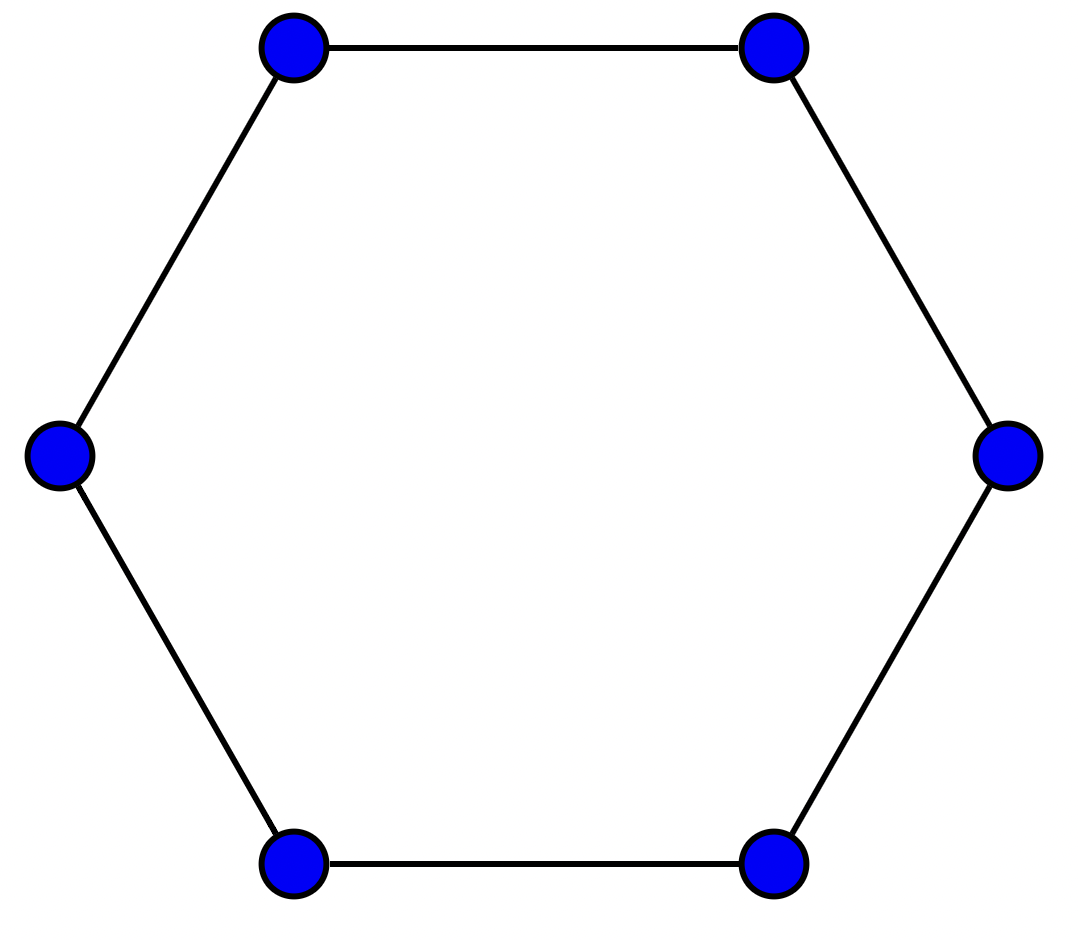
\includegraphics[scale=0.15]{Images/c_6.png}
    \caption{A picture of $C_6$}
\end{figure}

\begin{definition}
    Given a graph $G=(V,E)$, a \textbf{subgraph} of $G$ is a pair $H=(W,E')$ such that $W \subset V$ and $E' \subset \{s \in E: s \subset W\}$. 
    We sometimes abuse notation and write $H \subset G$.
\end{definition}


\begin{definition}
    Given a graph $G=(V,E)$, an \textbf{induced subgraph} is one of the form $$(W,\{\{x,y\} \in E: \{x,y\} \subset W\})$$
    where $W \subset V$
\end{definition}
\begin{figure}[ht]
    \centering
    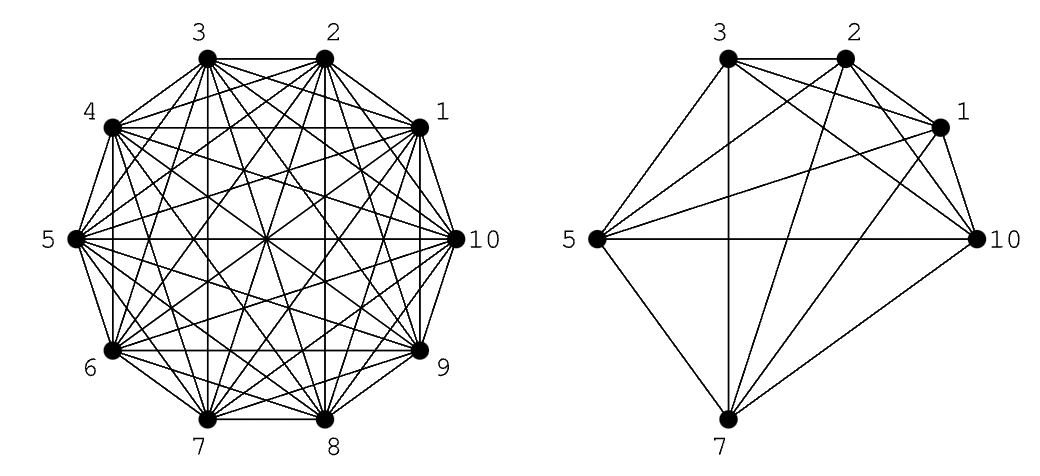
\includegraphics[scale=0.4]{Images/isb.png}
    \caption{A picture of induced subgraph}
\end{figure}
\textbf{Remark}:
\begin{itemize}
    \item Induced subgraphs are uniquely determined by the vertex set, while the standard subgraph is not.
\end{itemize}

\begin{definition}
    Let $G=(V_1,E_1)$ and $H=(V_2,E_2)$ be graphs. 
    We say $G$ and $H$ are \textbf{isomorphism} if there is a bijectiion $$f:V_1 \longrightarrow V_2$$
    with the property that $$\{x,y\} \in E_1 \Longleftrightarrow \{f(x),f(y)\} \in E_2$$
\end{definition}


\begin{theorem}
    Let $G$ be a graph with $n$ vertices. $G$ is isomorphic to a subgraph of $K_n$.
\end{theorem}
\textbf{Remark}:
\begin{itemize}
    \item The above is false if we require the subgraph be induced.
\end{itemize}


\begin{definition}
    Given a graph $G=(V,E)$, and a vertex $v \in V$, we let $$deg_G(v)=|\{u \in V: \{u,v\} \in E\}|$$
    Given a graph $G$, we can create a sequence $(deg_G(v): v \in V)$ of degrees called a \textbf{degree sequence}.
\end{definition}

\begin{theorem}
    Let $G$ and $H$ be graphs, and $f:G \longrightarrow H$ be an isomorphism. 
    Then $$deg_G(x)=deg_{H}(f(v))$$
\end{theorem}


\begin{corollary}
    If $G$ and $H$ have different degree sequences(under any possible ordering), then thsy are not isomorphic.
\end{corollary}

\begin{lemma}[The Handshaking Lemma]
    Let $G=(V,E)$ be a graph, and let $|E|=e$ then $$\sum_{v \in V}deg_G(v)=2e$$
\end{lemma}
\begin{proof}
    For each $v \in V$, let $E_v=\{\{u,v\}:\{u,v\}\in E\}$ denotes all edges around $v$. 
    Notice that for distinct $u,v$, $|E_u \cap E_v| \leq 1$.
    \begin{itemize}
        \item $|E_u \cap E_v| = 1$ when $u,v$ form an edge.
        \item No three distict sets overla.
    \end{itemize}
    It follows that
    \begin{equation}
        \begin{split}
            e &= |E|\\
            &=|\cup_{v \in V}E_v|\\
            &= \sum_{v \in V}|E_v| - \sum_{u,v \in V}|E_u \cap E_v|\\
            &= \sum_{v \in V}def_G(v)-e
        \end{split}
    \end{equation}
    Therfore, $\sum_{v \in V}deg_G(v)=2e$.
\end{proof}


\begin{definition}
    A \textbf{walk} of a graph $G$ is a sequence of vertices $x_1,\cdots,x_n$ that are each successively connected with an edge.
\end{definition}

\begin{definition}
    A \textbf{path} of a graph $G$ is a sequence of \underline{distinct} vertices $x_1,\cdots,x_n$ that are each successively connected with an edge. 
    We call the number of edges in the sequence the \textbf{length of the path}. 
\end{definition}


\begin{definition}
    We call a graph $G$ \textbf{connected} if every part of distinct vertices is connected by a path.
\end{definition}

\begin{definition}
    Given a graph $G$, we denote a maximally connected vertex set a \textbf{connected component}. 
    More formally, if we denote the equivalence relation $\sim$ on $V$ given by $v \sim w \Longleftrightarrow v=w$ or $v$ is connected to $w$. 
    The connected components are the equivalent classes given by this relation.
\end{definition}
\begin{figure}[ht]
    \centering
    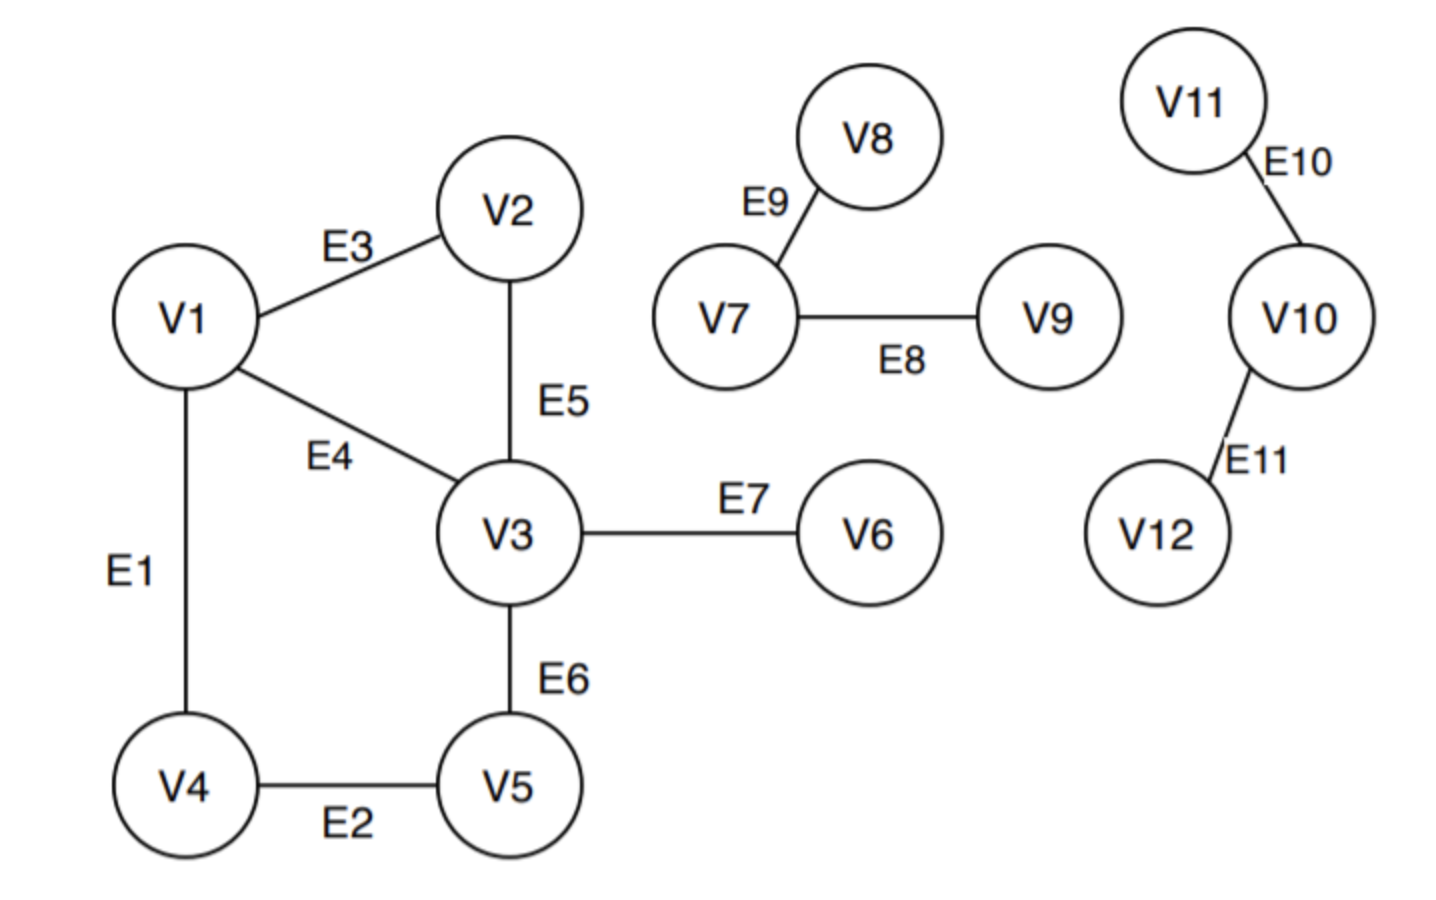
\includegraphics[scale=0.3]{Images/3components.png}
    \caption{A picture of a graph with 3 components}
\end{figure}
\textbf{My Question}:
\begin{itemize}
    \item What is the relation between this and the connected component in topology?
    \item A graph $G$ is a structured set, what is the topology for this set?
\end{itemize}



\section{Trees}

\begin{definition}
    A \textbf{tree} is a graph $G=(V,E)$ with the property that every two vertices are connected by a \underline{unique} path.
\end{definition}
\textbf{Remark}:
\begin{itemize}
    \item The definition implies a tree is connected.
    \item Trees are the minimally connected objects.
\end{itemize}
\begin{figure}[ht]
    \centering
    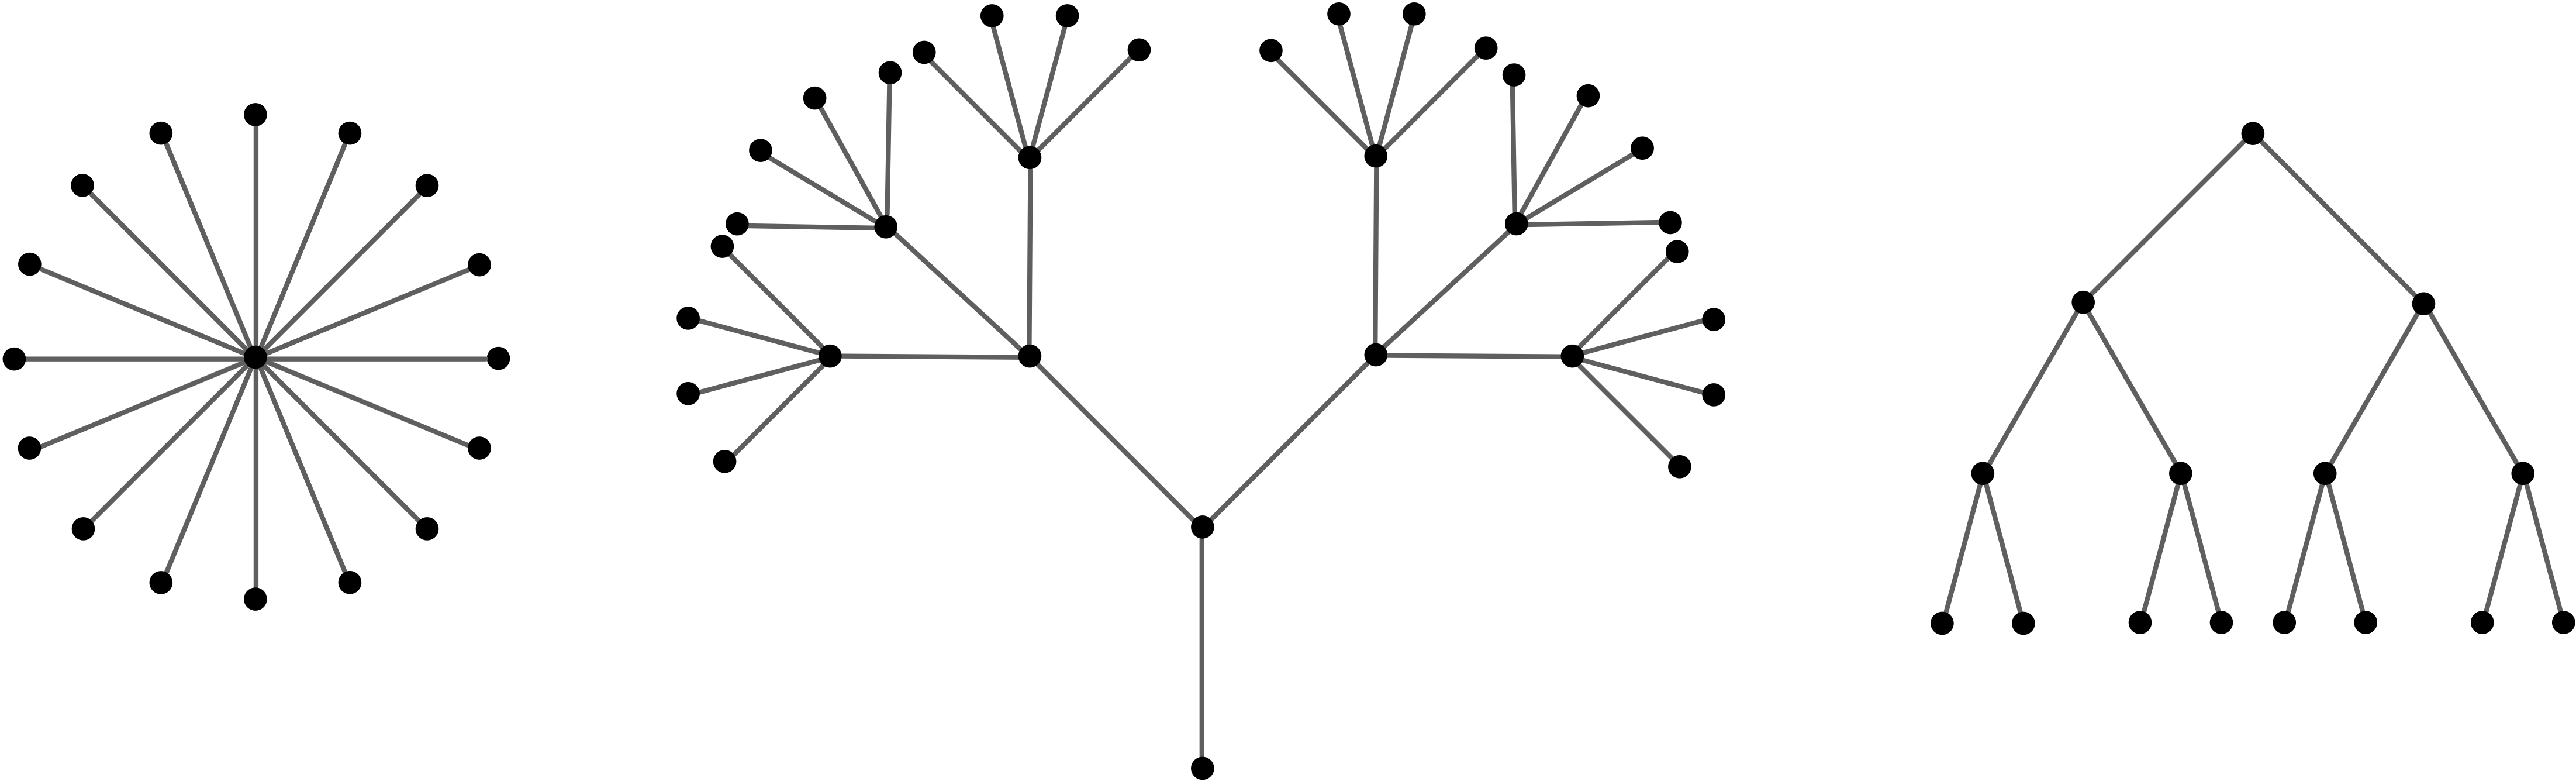
\includegraphics[scale=0.15]{Images/forest.png}
    \caption{A picture of 3 trees}
\end{figure}

In order to prove the next theorem, we need the following lemmas.

\begin{lemma}
    If $G=(V,E)$ is connected and has no cycle, then $$\exists v \in V. deg_V(v)=1$$
    (For any vertex $v$ hs such property will be called a \textbf{leaf}.)
\end{lemma}
\begin{proof}
    (Prove by contradiction.)\\
    Let $G=(V,E)$ be a connected graph with $n$ vertices and has no cycle. Suppose $\forall v \in V. deg_V(v) \geq 2$.
    Consider the procedure:
    \begin{itemize}
        \item Set $i=2$. Select any vertex to be $v_1$, and trace an edge $e_1$ from $v_1$ to some neighboring vertex $v_2$.
        (This is possible because the tree has at least 2 vertices and is connected.)
        \item From $v_i$, trace $e_i \neq e_{i-1}$ to $v_{i+1} \neq v_i$.
        \item Set $i \mapsto i+1$. Repeat from step2.
    \end{itemize}
    \begin{figure}[ht]
        \centering
        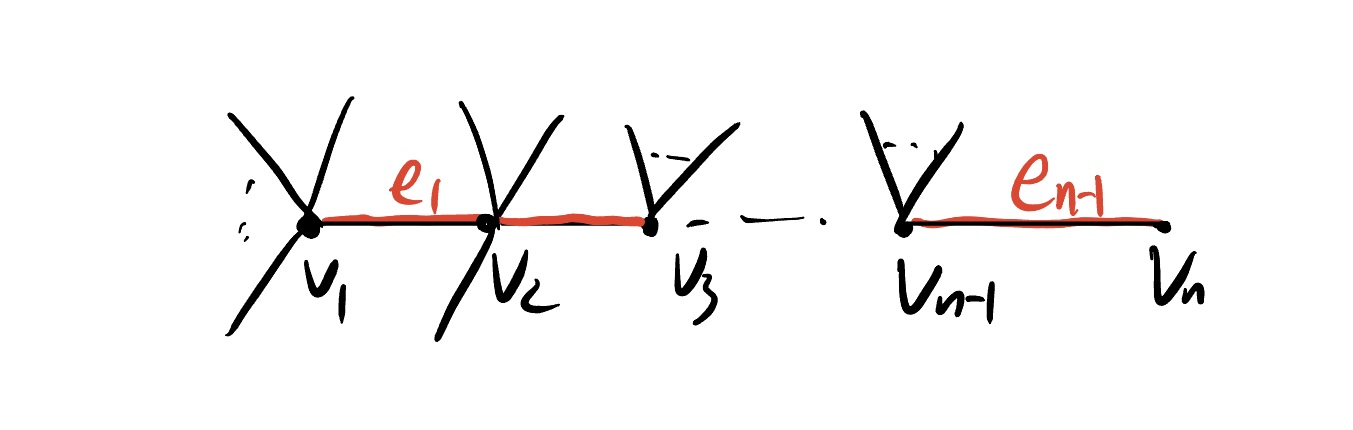
\includegraphics[scale=0.14]{Images/lemma_pic.jpg}
        \caption{A picture of applying the lemma}
    \end{figure}
    Hence for $v_n$, there must be an $e_n$, connecting one of $\{v_1,\cdots,v_{n-1}\}$.\\
    Therefore, we have a cycle. This is a contradiction.
\end{proof}



\begin{lemma}[Characterisation of bridge]
    An edge $e$ of a graph $G$ is a bridge if and only if $e$ lies on no cycle of $G$.
\end{lemma}


\begin{theorem}
    Let $G$ be a connected graph with $n$ vertices. The following are equivalent.
    \begin{enumerate}
        \item $G$ is a tree.
        \item $G$ does not contain a cycle.
        \item $G$ has $n-1$ edges.
    \end{enumerate}
\end{theorem}
\begin{proof}
    We are going to show that
    $$(1) \Longrightarrow (2) \Longrightarrow (3) \Longrightarrow (1)$$
    \begin{enumerate}
        \item Suppose $G$ is a tree. Suppose there is a cycle $x_1,x_2,\cdots,x_n$ with $\{x_i,x_{i+1}\}$ and $\{x_n,x_1\}$. 
        Notice, 
        \begin{itemize}
            \item $x_1,\cdots,x_n$ is a path from $x_1$ to $x_n$.
            \item $x_1,x_n$ is also a path from $x_1$ to $x_n$.
        \end{itemize}
        This contradicts to uniqueness.
        \item Let $n$ be the number of vertices, we are going to do induction on $n$.\\
        Base case:$n=1$, there is 0 edge, true.\\
        Inductive step: Assume $(2) \Longrightarrow (3)$ is true for $n$. 
        Let $G=(V,E)$ be a connected graph with $n+1$ vertices with no cycle. 
        By the first lemma, there exists $v_k$ that has only one edge. 
        Let $\{v_t,v_k\}$ denotes that edge. Remove $v_k$ and $\{v_t,v_k\}$ from $G$. Can show easily that the new graph $G'$ is connected. (Since $\forall v_p,v_q \in V$, there exists a path from $v_p$ to $v_q$ and $v_k$ cannot be in this path, otherwise there will have repetition.)
        By induction hypothesis, $G'$ has $n-2$ edges. Therefore, $G$ has $n-1$ edges.
        \item Do strong induction on number of vertices $n$.\\
        Base case: $n=1$, true.\\
        Inductive step: Assume $(3) \Longrightarrow (1)$ is true for $n$. 
        Let $G$ be a connected graph on $n+1$ vertices with $n$ edges. 
        If $G$ has cycle, then there are at least $n+1$ edges. This is a contradiction, hence $G$ has no cycle. 
        Pick any edge $\{v_p,v_q\}$ from $G$. 
        By the second lemma, $\{v_p,v_q\}$ is a bridge. 
        Remove this bridge, by definition of bridge, we have two connected components. 
        Let us denote them as $G_1=(V_1,E_1),G_2=(V_2,E_2)$, $V=V_1 \coprod V_2$. 
        For any $u,v \in V$
        \begin{itemize}
            \item $u,v$ both in $V_1$ or $V_2$. By induction hypothesis, we are done.
            \item $u,v$ in different connected components. Without loss of generality, assume $u \in V_1,v \in V_2$. 
            By induction hypothesis, there is a unique path from $u$ to $v_p$ in $G_1$, and a unique path from $v_p$ to $v$ in $G_2$. 
            Connected two paths with $\{v_p,v_q\}$, we have a unique path from $u$ to $v$ in $G$.
        \end{itemize}
    \end{enumerate}
\end{proof}


\begin{definition}
    Let $T=(V,E)$ be a tree. We call a vertex $v$ a \textbf{leaf} if $deg_T(v)=1$.
\end{definition}

\begin{lemma}
    Let $T$ be a tree with at least 2 vertices, then $T$ has atleast two leaves.
\end{lemma}

\begin{definition}
    Given a graph $G=(V,E)$, we call a subgraph $H \subset G$ \textbf{spanning} if $H=(V,E')$ where $E' \subset E$.
\end{definition}

\begin{definition}
    Given a graph $G$, a \textbf{spanning tree} is a subgraph $T \subset G$ that is a tree.
\end{definition}

\begin{theorem}
    Every connected graph has a spanning tree.
\end{theorem}

\noindent \textbf{Questions}:Prove:
\begin{itemize}
    \item A graph is connected $\Longleftrightarrow$ it has a spanning tree.
    \item $G$ is a tree $\Longleftrightarrow$ the removal of any edge disconnects $G$.
\end{itemize}

\begin{definition}
    A \textbf{labeled tree} is a tree $T$ whose vertex set is $\{1,\cdots,n\}$.i.e. The vertex set is ordered.
\end{definition}

\begin{definition}[\textbf{Algorithm to convert a Prüfer sequence into a tree}]
    Fix $n \geq 2$, let $s:[n-2] \longrightarrow \{1,\cdots,n\}$ be a sequence.
    ($s$ is a sequence that has length $n-2$ ,every digit is a number from 1 to $n$)
    Consider the following algorithm that generates a set $E$ of size $k-1$
    \begin{itemize}
        \item Find the smallest $j$ which is not in the range of $s$(find the smallest number in$\{1,\cdots,n\}$ that we didn't use.)
        Put $\{j,s(0)\}$ in $E$. Set $L=\{1,\cdots,n\} \setminus \{j\}$ and delete the first entry of the sequence to get a new sequence $s$
        \item Suppose we 're at a stage $i$. Find the smallest $j$ in $L$ that is not in the range sequence. 
        Add $\{j,s(0)\}$ to $E$ (recall $s(0)$ may be different now as we 're truncated $s$). Remove $j$ from $L$ 
        and truncate $s$ by removing the first entry again.
        \item When the string $s$ is empty, $L$ contains two elements. Add $L$ to $E$.
    \end{itemize}
\end{definition}
\textbf{Remark}:
\begin{itemize}
    \item The above assigns each sequence $s$, a set $E$ of size $n-1$, such that the associated graph $(\{1,\cdots,n\},E)$ is connected
\end{itemize}
\begin{figure}[ht]
    \centering
    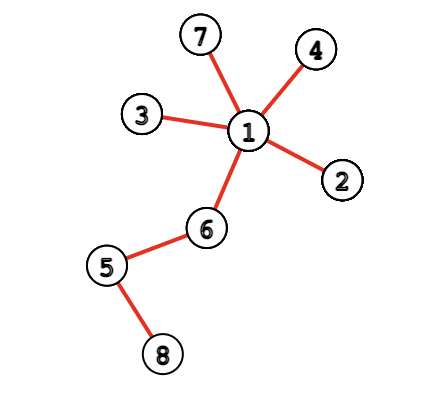
\includegraphics[scale=0.5]{Images/pfc111165.png}
    \caption{Prüfer Code: 111165}
\end{figure}



\begin{definition}[\textbf{Algorithm to convert a tree into a Prüfer sequence}]
    Suppose we have a labeled tree $T=(\{1,\cdots,n\},E)$. 
    We associated to $T$ a sequence $s:[n-2] \longrightarrow \{1,\cdots,n\}$ defined as follows:
    \begin{itemize}
        \item $s(0)$ is the unique vertex adjacent to the leaf witthe smallest indes. Delete this leaf and move to the nest stage.
        \item $s(i)$ is the unique vertex adjacent to the leaf with the smallest index in the new tree gotten from deleting the last leaf.
        \item The process will terminate when the tree becomes a single edge with two leaves.
    \end{itemize}
\end{definition}
\textbf{Remark}:
\begin{itemize}
    \item To each labeled tree, there is a unique Prüfer code associated to it.
\end{itemize}


\begin{theorem}[Cayley]
    For each $n \geq2$, there are exactly $n^{n-2}$ labeled trees on $\{1,\cdots,n\}$
\end{theorem}
\begin{proof}
    To each tree, find the unique associated Prüfer code $s:[n-2] \longrightarrow \{1,\cdots,n\}$. 
    This puts labeled trees in bijective correspondence with sequences $s$. 
    There are exactly $n^{n-2}$ such sequences. Hence exactly many trees. 
\end{proof}


\section{Eulerian Graphs}

\begin{definition}
    Given a graph $G=(V,E)$, an \textbf{Eulerian circuit} is a sequence of vertices $x_0,\cdots,x_t$ with the property that:
    \begin{itemize}
        \item $x_0=x_t$
        \item $\forall i \in [t]. \{x_i,x_{i+1}\} \in E$
        \item $\forall e \in E. \exists i \in [t]. e=\{x_i,x_{i+1}\}$ and this choice is unique. i,e, every edge appears exactly once.
    \end{itemize}
\end{definition}
\textbf{Remark}:
\begin{itemize}
    \item The reason why the Eulerian path came up with, is initially solve the problem: \underline{Bridges of Könisberg}.
\end{itemize}
\begin{figure}[ht]
    \centering
    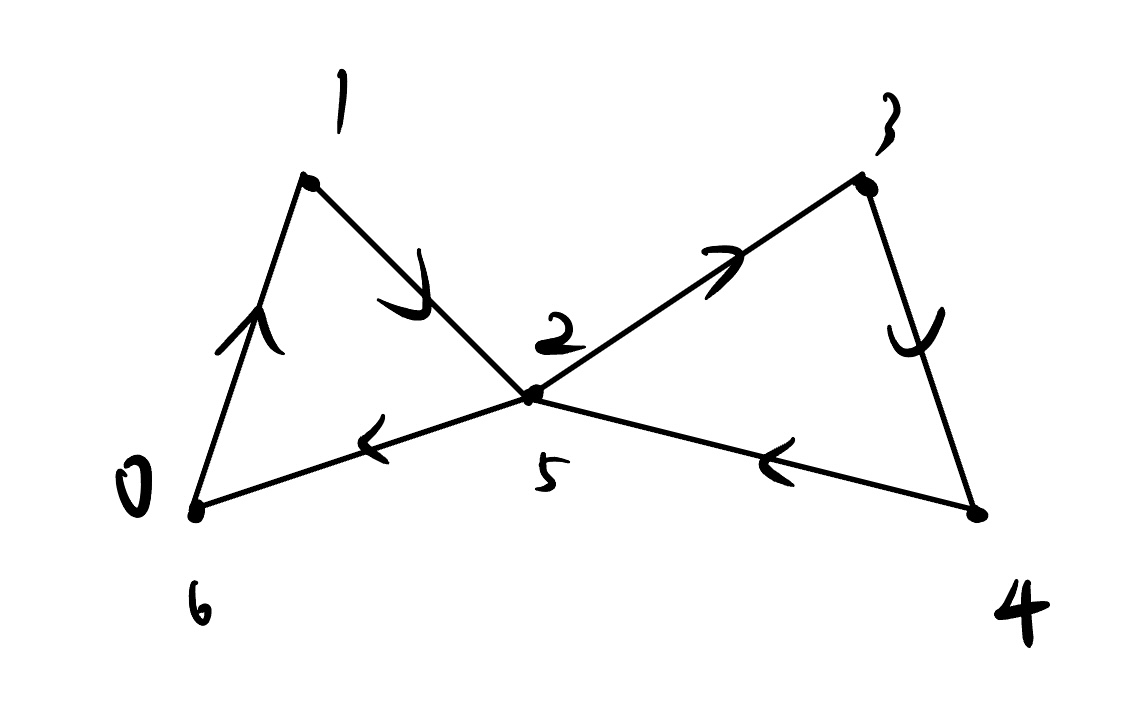
\includegraphics[scale=0.125]{Images/circuit.jpg}
    \caption{A picture of a circuit}
\end{figure}


\begin{definition}
    An \textbf{Eulerian graph} is a graph containing an eulerian circuit.
\end{definition}

\begin{theorem}
    A connected graph $G=(V,E)$ is Eulerian if and only if all its vertices have even degree.
\end{theorem}
\begin{proof}
    (Only If)\\
    Assume $G$ is Eulerian. Note that in an Eulerian trail, for every vertex $v$, each time we enter the vertex, we must leave.(else we've stuck). 
    Hence the vertex must be of even degree.\\
    (If)\\
    Strong induction on the number of edges.\\
    Base case: $t=0$ edges, it is trivial.\\
    Inductive step: Assume for all graphs with $<t$ many edges the if direction is true. 
    Take a connected graph $G=(V,E)$ with $t$ edges. 
    By the procedure defined in the last section, we can prove that $G$ has a cycle subgraph $(\{x_1,\cdots,x_k\},E')$. 
    Consider the connected components of the graph $(V,E \setminus E')$ call them $S_1,\cdots,S_m$.
    \begin{figure}[ht]
        \centering
        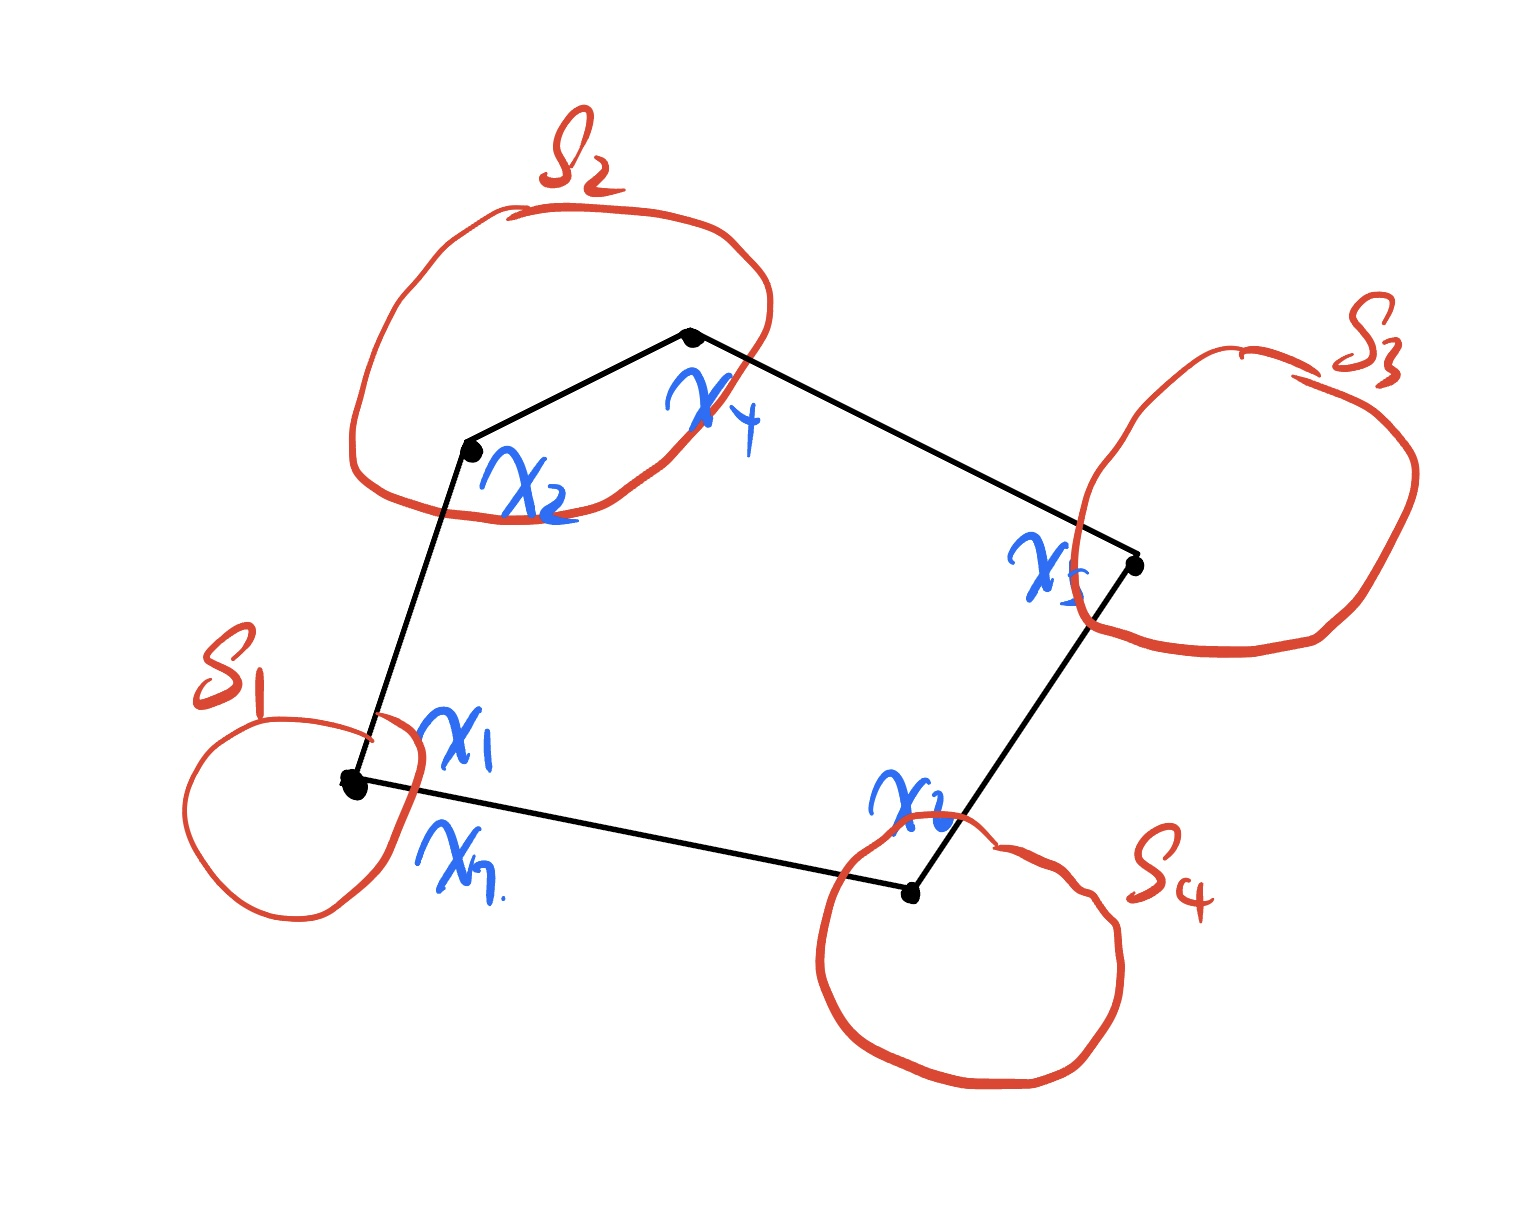
\includegraphics[scale=0.125]{Images/IMG_0298.jpg}
        \caption{A picture discription of our proof}
    \end{figure}
    Start with $x_1$ and the component it is in. Can find an Eulerian circuit back to $x_1$.
    Move from $x_1$ to $x_2$ along the edge $\{x_1,x_2\} \in E'$. 
    If $x_2$ and $x_1$ are in the same connected component, move to $x_3$ and reiterate the argument, else apply induction hypothesis again. 
    We've recursively constructed a sequence $x_1,\cdots,x_1,x_t,\cdots,x_t,\cdots,x_p,\cdots,x_p$ that walks over every edge. 
\end{proof}


\section{Hamiltonian Graphs}

\begin{definition}
    A \textbf{cycle} in a graph $G$ is a sequence of distinct vertices $v_1,\cdots,v_k$ such that for $i \in \{1,\cdots,k-1\}. \{v_i,v_{i+1}\} \in E$ and $\{v_k,v_1\} \in E$.
\end{definition}
\textbf{Note}:
\begin{itemize}
    \item A cycle induces a copy of a subgraph isomorphic to $C_k$ when $k \geq 3$.
    \item We allow for a one point cycle.
\end{itemize}

\noindent \textbf{Remark*}:
\begin{itemize}
    \item Walk: Vertices may repeat. Edges may repeat.(Closed or Open)
    \item Trail: Vertices may repeat. Edges cannot repeat.(Open)
    \item Circuit: Vertices may repeat. Edges cannot repeat.(Closed)
    \item Path: Vertices cannot repeat. edges cannot repeat.(Open)
    \item Cycle: Vertices cannot repeat. Edges may repeat.(Closed)
\end{itemize}

\begin{definition}
    We call a graph with $n$ vertices \textbf{Hamiltonian} if it admits a cycle of length $n$. i.e. it has a spanning subgraph that is isomorphic to $C_n$.
\end{definition}
\begin{figure}[ht]
    \centering
    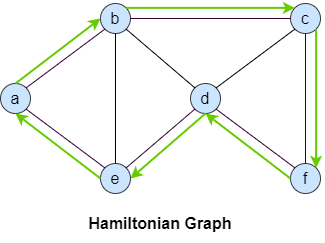
\includegraphics[scale=0.45]{Images/hamiltonian.png}
    \caption{A picture of a Hamiltonian graph}
\end{figure}



\begin{theorem}[Sufficient condition for hamiltonian]
    Let $G=(V,E)$ be a graph with $n$ vertices. Suppose that $\forall v \in V.deg(v) \geq \lceil \frac{n}{2} \rceil$. Then $G$ is Hamiltonian.
\end{theorem}
\begin{proof}
    Since the graph $G$ is finite. We can take a maximal path $v_1,\cdots,v_k$. 
    Note, it must be the case that all the vertices adjacent to $v_1$ or $v_k$ excluding possible each other must be in the sequence $v_2,\cdots,v_{k-1}$. Else we can extand the sequence getting a contradiction.
    There is a $j \in \{2,\cdots,k-1\}$ such that $\{v_1,v_{j-1}\},\{v_j,v_k\} \in E$. 
    If not, (i.e. $\forall j \in \{2,\cdots,k-1\}.\{v_1,v_{j+1}\} \notin E \text{ or } \{v_j,v_k\} \notin E.$) there are $deg(v_1)$ vertices adjacevt to $v_1$. 
    Hence there are $deg(v_1)=\lceil \frac{n}{2} \rceil$ vertices not adjacent to $v_k$. 
    Therefore, there are at least $deg(v_1)+deg(v_k)=\lceil \frac{n}{2} \rceil + \lceil \frac{n}{2}\rceil \geq n$ vertices. 
    Include $v_k$, there are at least $n+1$ vertices. Contradiction.
    \begin{itemize}
        \item It follows that $v_1,\cdots,v_j,v_k,v_{k-1},\cdots,v_{j+1}$ is a cycle.
        \item It follows that every vertex must be on the cycle, else starting from the vertex and moving into the cycle we can create a path of length $>k$.
        \begin{figure}[ht]
            \centering
            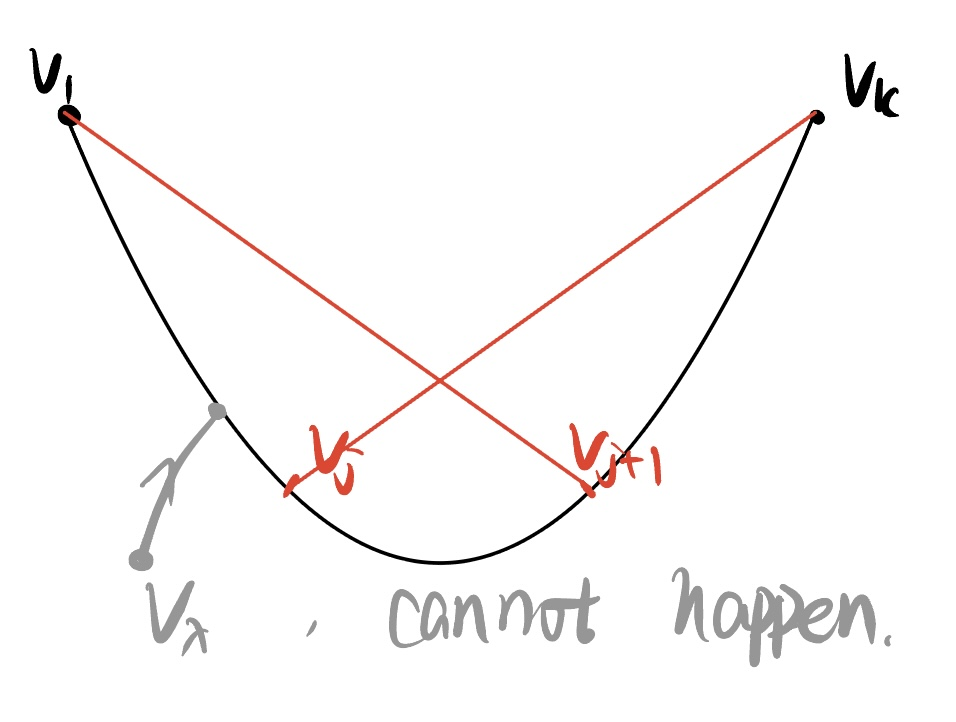
\includegraphics[scale=0.13]{Images/IMG_0299.jpg}
            \caption{A picture discription of the proof}
        \end{figure}
        
    \end{itemize}
\end{proof}


\section{Graph Coloring}

\begin{definition}
    Given a graph $G=(V,E)$, we say $A \subset V$ is \textbf{independent} if and only if no two vertices in $V$ are adjacent.
\end{definition}
\begin{figure}[ht]
    \centering
    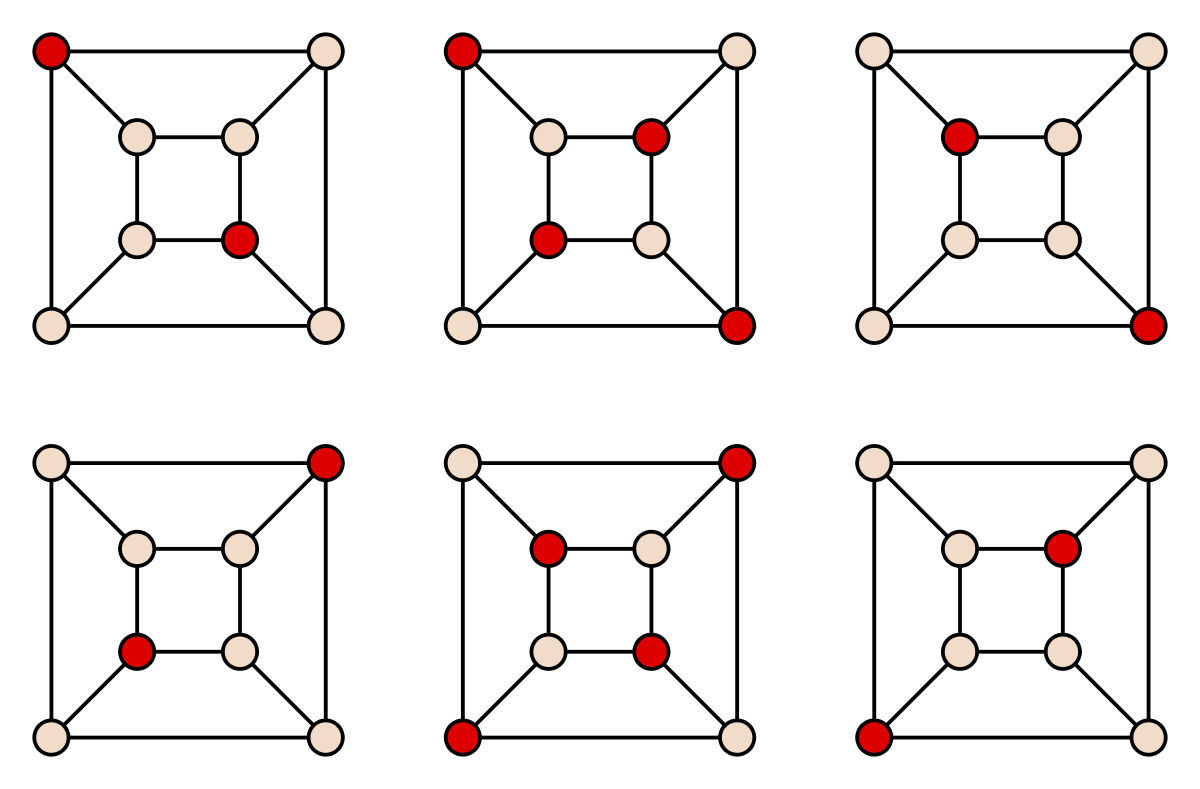
\includegraphics[scale=0.14]{Images/1200px-Cube-maximal-independence.svg.png}
    \caption{A picture independent parts}
\end{figure}
\textbf{Remark}:
\begin{itemize}
    \item If we think the graph that represent the relations of people, then the independent set represent a set of people who don't know each other.
    \item Can show that the only independent sets in $K_n$ are singletons.
\end{itemize}

\begin{definition}
    We say a graph $G=(V,E)$ is \textbf{bipartite} if and only if we can partition $V$ into two disjoint independent sets.
\end{definition}
\textbf{Question}:
\begin{itemize}
    \item Show that a graph is bipartite if and only if it does not contain a cycle of odd length.
\end{itemize}
\begin{figure}[ht]
    \centering
    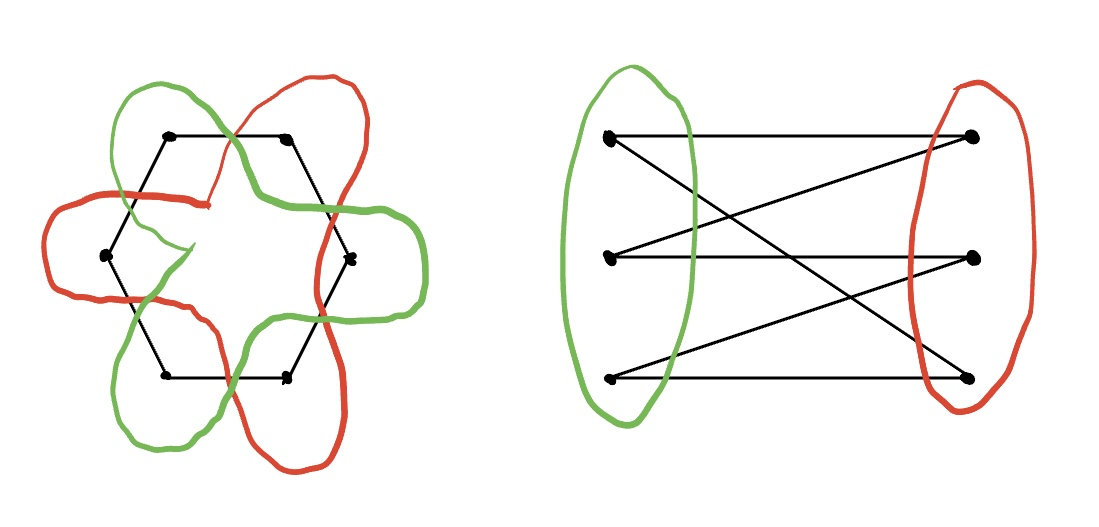
\includegraphics[scale=0.2]{Images/IMG_0300.jpg}
    \caption{A picture bipartite graphs}
\end{figure}

\begin{definition}
    A \textbf{complete bipartite graph} $K_{n,m}=([n]\cup[m],E)$ is a special bipartite graph where every vertex of the $[n]$ is connected to every vertex of $[m]$ and vice versa.
\end{definition}
\begin{figure}[ht]
    \centering
    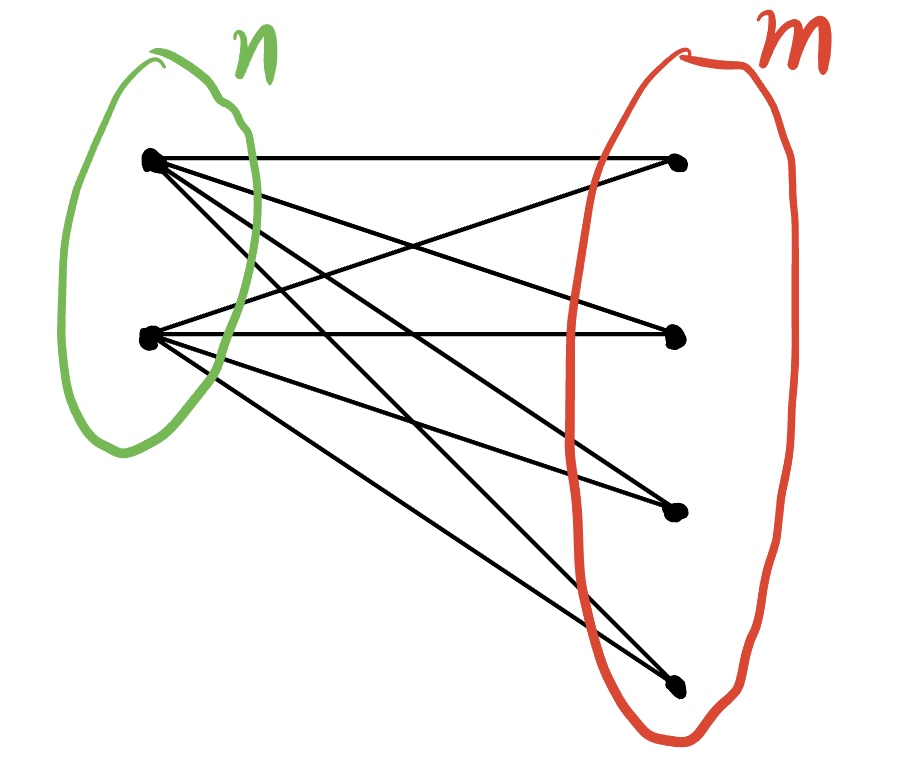
\includegraphics[scale=0.14]{Images/IMG_0301.jpg}
    \caption{A picture of $K_{2,4}$}
\end{figure}


\begin{definition}
    Let $G=(V,E)$ be a graph. A \textbf{(proper) colouring} of $G$ is a function $$\phi:V \longrightarrow [k]$$
    such that for all $i \in [k]$, $\phi^{-1}(i)$ is independent. 
    Equivalently, if $\{a,b\}\in E$,$\phi(a) \neq \phi(b)$, we call $\phi$ a \textbf{k-colouring}.
\end{definition}
\begin{figure}[ht]
    \centering
    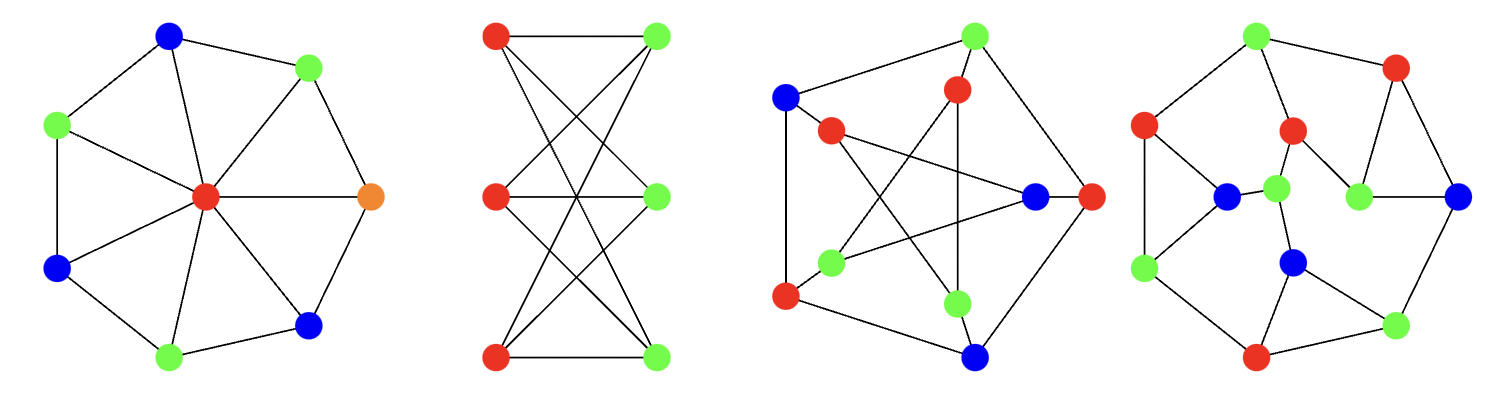
\includegraphics[scale=0.35]{Images/colouring.png}
    \caption{A picture of colouring}
\end{figure}


\begin{definition}
    \textbf{The chromatic number} of a graph $G$, is the smallest $k$ such that there is a proper k-colouring of $G$. 
    We denote this number \underline{$\chi(G)$}
\end{definition}

\begin{definition}
    We say a graph $G$ is \textbf{planar} if there exists a depiction of it on a plane without any edge crossing.(i.e. you can draw it on a piece of paper with no edge crossing)
\end{definition}
\textbf{Remark}:
\begin{itemize}
    \item The above should feel unsatisfactory due to lack of mathematical rigidity. This issue is solved thanks to Kuratowski.
    \item The key inthe above definition is the existence.
\end{itemize}
\begin{figure}[ht]
    \centering
    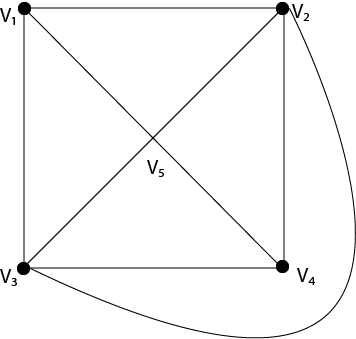
\includegraphics[scale=0.3]{Images/planar-and-non-planar-graphs2.png}
    \caption{$K_4$ is planar}
\end{figure}
\textbf{Real world applications}:
\begin{itemize}
    \item In computer science, there is a notation of \underline{thickness} that correlates planarity to how difficult a network is to embed.
    $$\text{\underline{How many planar pieces I can cover a graph with.}}$$
    For optimization problems, if you have a complicated network or a system that you need to embed on a plane or some circuit board, you should know how many boards you need,
    \item Questions of circuitry lines or wires are not allowed to cross are questions on planarity.(when the circuits must be embedded or built into a relatively 2D configuration)
\end{itemize}

\begin{definition}
    A \textbf{face} is a region bounded by edges in a planar depiction
\end{definition}
\begin{figure}[ht]
    \centering
    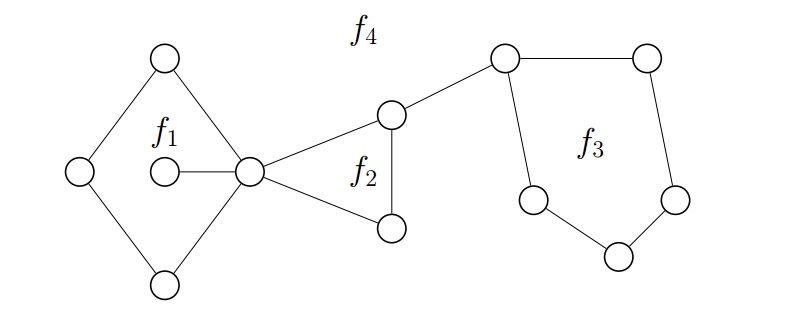
\includegraphics[scale=0.4]{Images/lrgtF.jpg}
    \caption{A planar embedding with 4 faces}
\end{figure}
\textbf{Remark}:
\begin{itemize}
    \item There is a basis of non-planar graphs.
\end{itemize}

\begin{definition}[Euler's Formula]
    Given a connected planar graph $G$ with $n$ vertices, $m$ edges, and $f$ faces. Then $$n-m+f=2$$
\end{definition}
\begin{proof}
    Do induction on $m$.\\
    Base case: $m=0$, the graph is a singleton. $1-0+1=2$ as desired.\\
    Inductive step: Suppose the assertion is true for graphs with $m$ edges. 
    Suppose $G$ is a graph with $m+1$ edges.
    \begin{itemize}
        \item If we can remove an edge in such a manner that keeps the graph connected, said edge must divide some face into two,so we get a new graph with $n$ vertices, $m$ edges and $f'=f-1$ faces. 
        By induction hypothesis, $n-m+f-1=2$. Hence we have $n-(m+1)+f=2$.
        \item Else, the graph is a tree and we're done as trees have 1 face.(the outer face, and any other face generates a cycle).
    \end{itemize}
\end{proof}

\begin{corollary}
    Let $G$ be a planar graph with $n \geq 3$ vertices and $m$ edges. We have the bound $$m \leq 3n-6$$
\end{corollary}
\begin{proof}
    Suppose the graph is connected and not a tree. (As it is trivial in the case for tree $m=n-1<3n-6$ for $n \geq3$)
    Let $S$ be the collection of pairs $(e,F)$ where $e$ is an edge and $F$ is a face.
    \begin{figure}[ht]
        \centering
        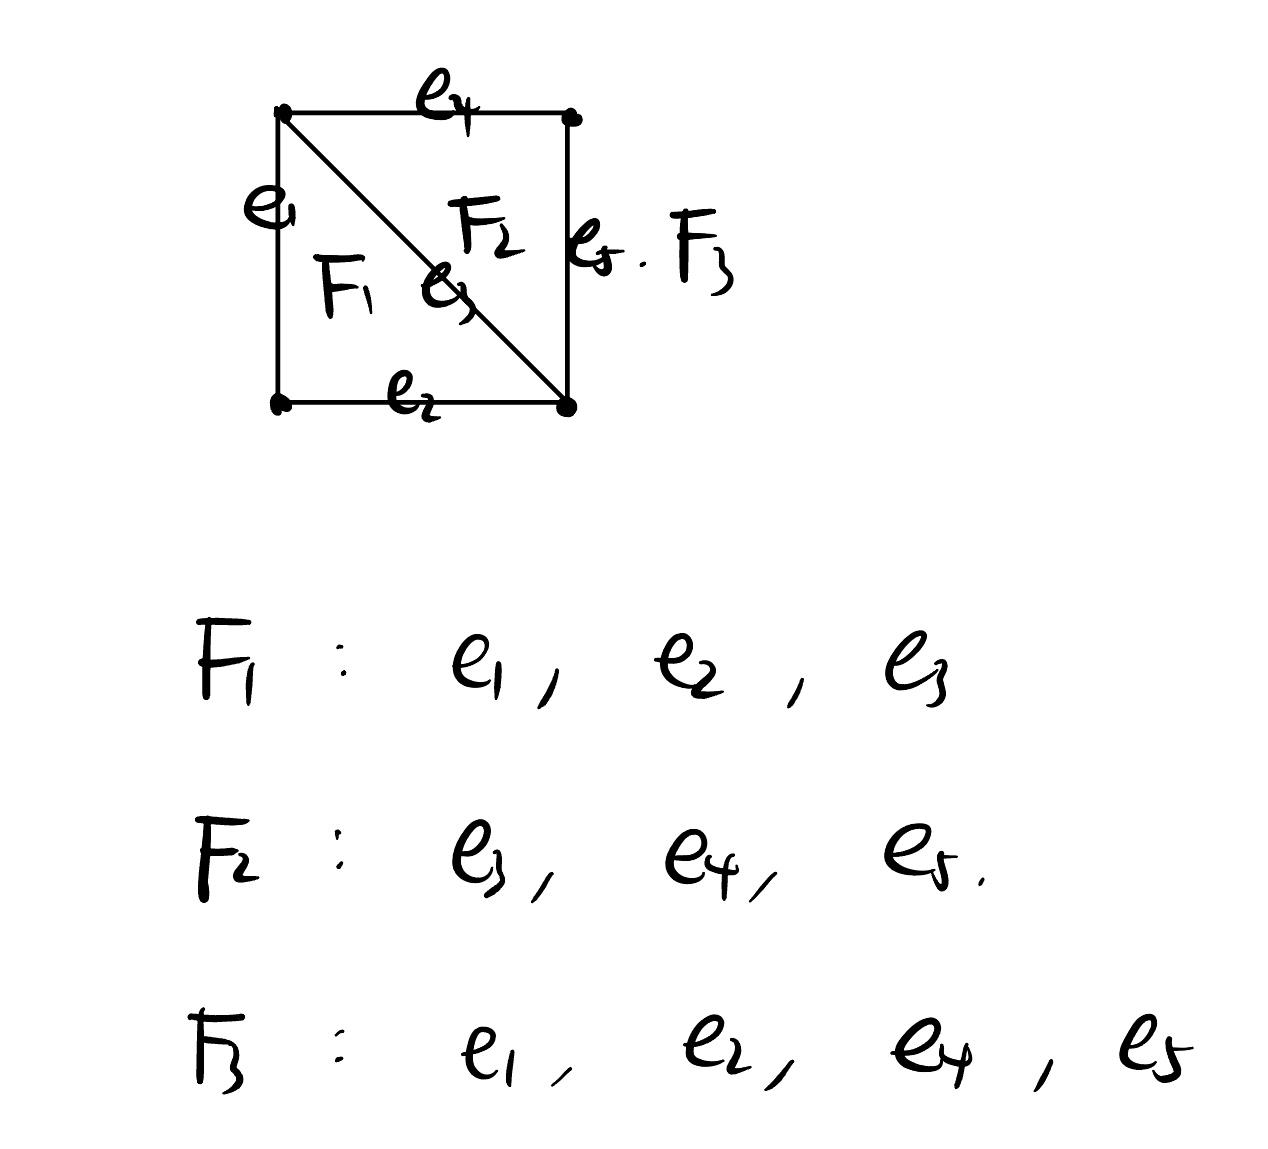
\includegraphics[scale=0.15]{Images/IMG_0303.jpg}
        \caption{A picture discription}
    \end{figure}
    \begin{itemize}
        \item For a fixed $e$, $|\{F:(e,F)\in S\}| \leq2$ as an edge borders at most 2 faces.
        \item For a ficed $F$, $|\{e: (e,F)\in S\}| \geq 3$
    \end{itemize}
    It follows that $3f \leq|S|\leq 2m$. By Euler's formula $$m=n+f-2 \leq n +\frac{2}{3}m-2$$
    This implies $m \leq 3n-6$. Complete proof in case of disconnectivity.(Breaking into connected components, and using the above)
\end{proof}
\textbf{Remark}:
\begin{itemize}
    \item Can use this to decide whether a graph is planar. For $K_5$, $m=10 >3\times5-6=9$, so $K_5$ is not planar.
\end{itemize}

\begin{definition}
    Let $G=(V,E)$ be a graph and take $e \in E$ and edge(set of 2 vertices). 
    A \textbf{contraction along e} is a graph $G'=((V\setminus e)\cup \{e\}, E')$
    where we say for all $u,v \in V \setminus e$, 
    $$\{u,v\}\in E \Longleftrightarrow \{u,v\}\in E'$$ and
    $$\{u,e\}\in E' \Longleftrightarrow \exists x \in e. \{u,x\}\in E$$
\end{definition}
\begin{figure}[ht]
    \centering
    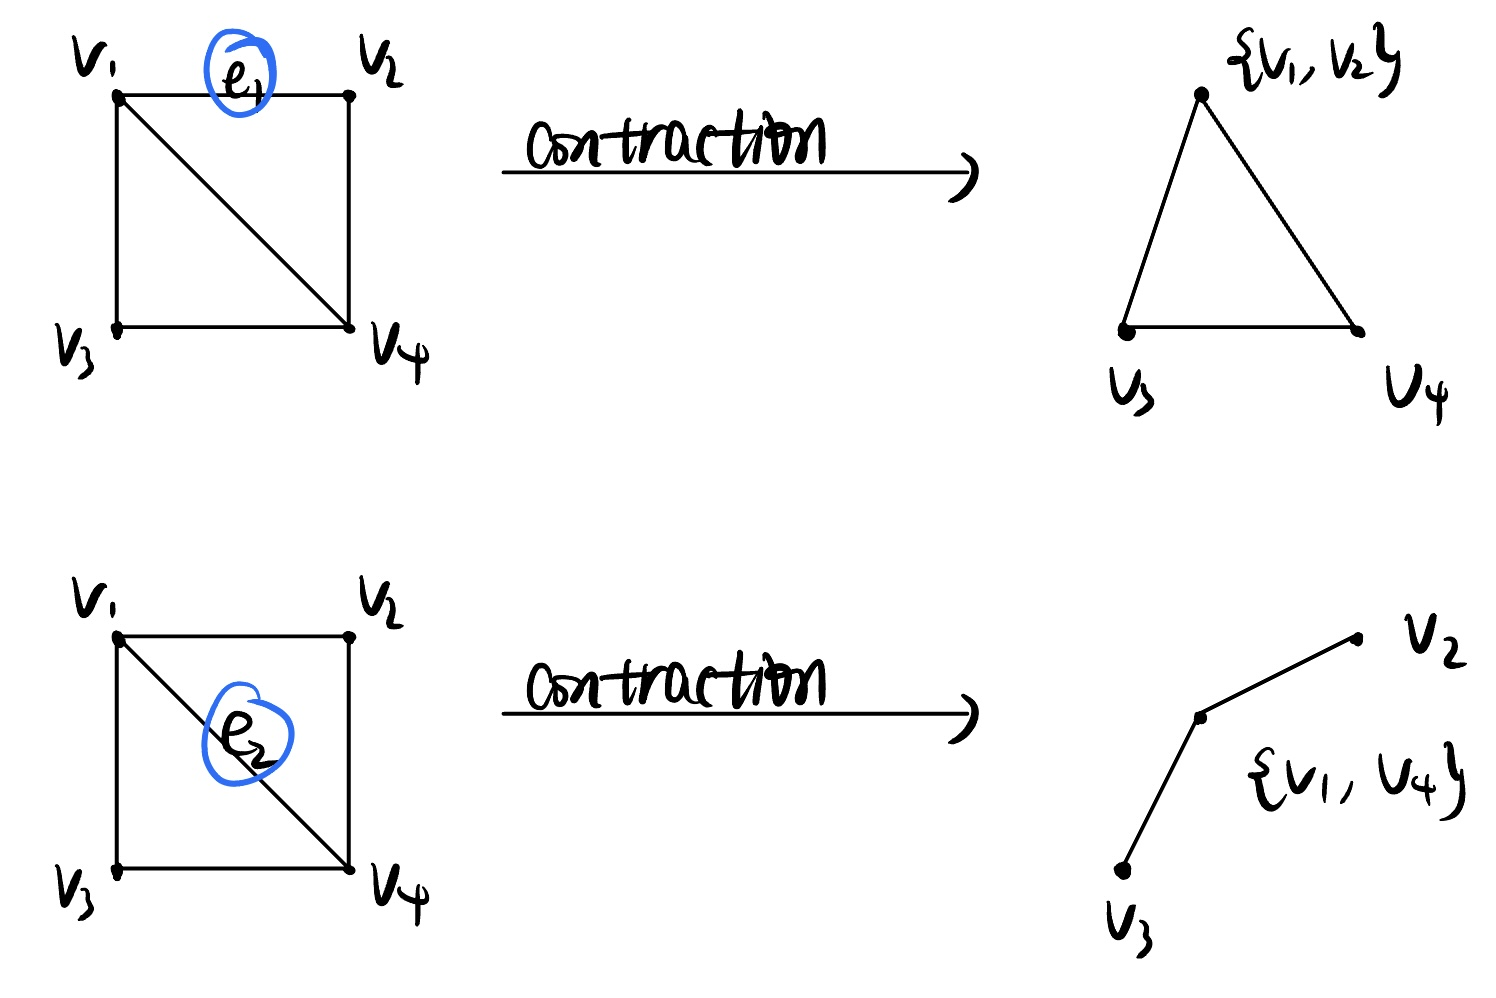
\includegraphics[scale=0.15]{Images/IMG_0304.jpg}
    \caption{A picture of contraction}
\end{figure}
\textbf{Remark}:
\begin{itemize}
    \item The essence is taking two vertices on that edge, and suck them together, Some people refer this as \underline{smoothing}.
\end{itemize}

\begin{definition}
    A \textbf{graph minor} of a graph $G$ is a graph $H$ gotten via a process of taking subgraphs and contractions.
\end{definition}

\begin{theorem}[Kuratowski]
    A graph is planar if and onlt if it does not contain a copy of $K_5$ or $K_{3,3}$ as a minor.
\end{theorem}
\begin{figure}[ht]
    \centering
    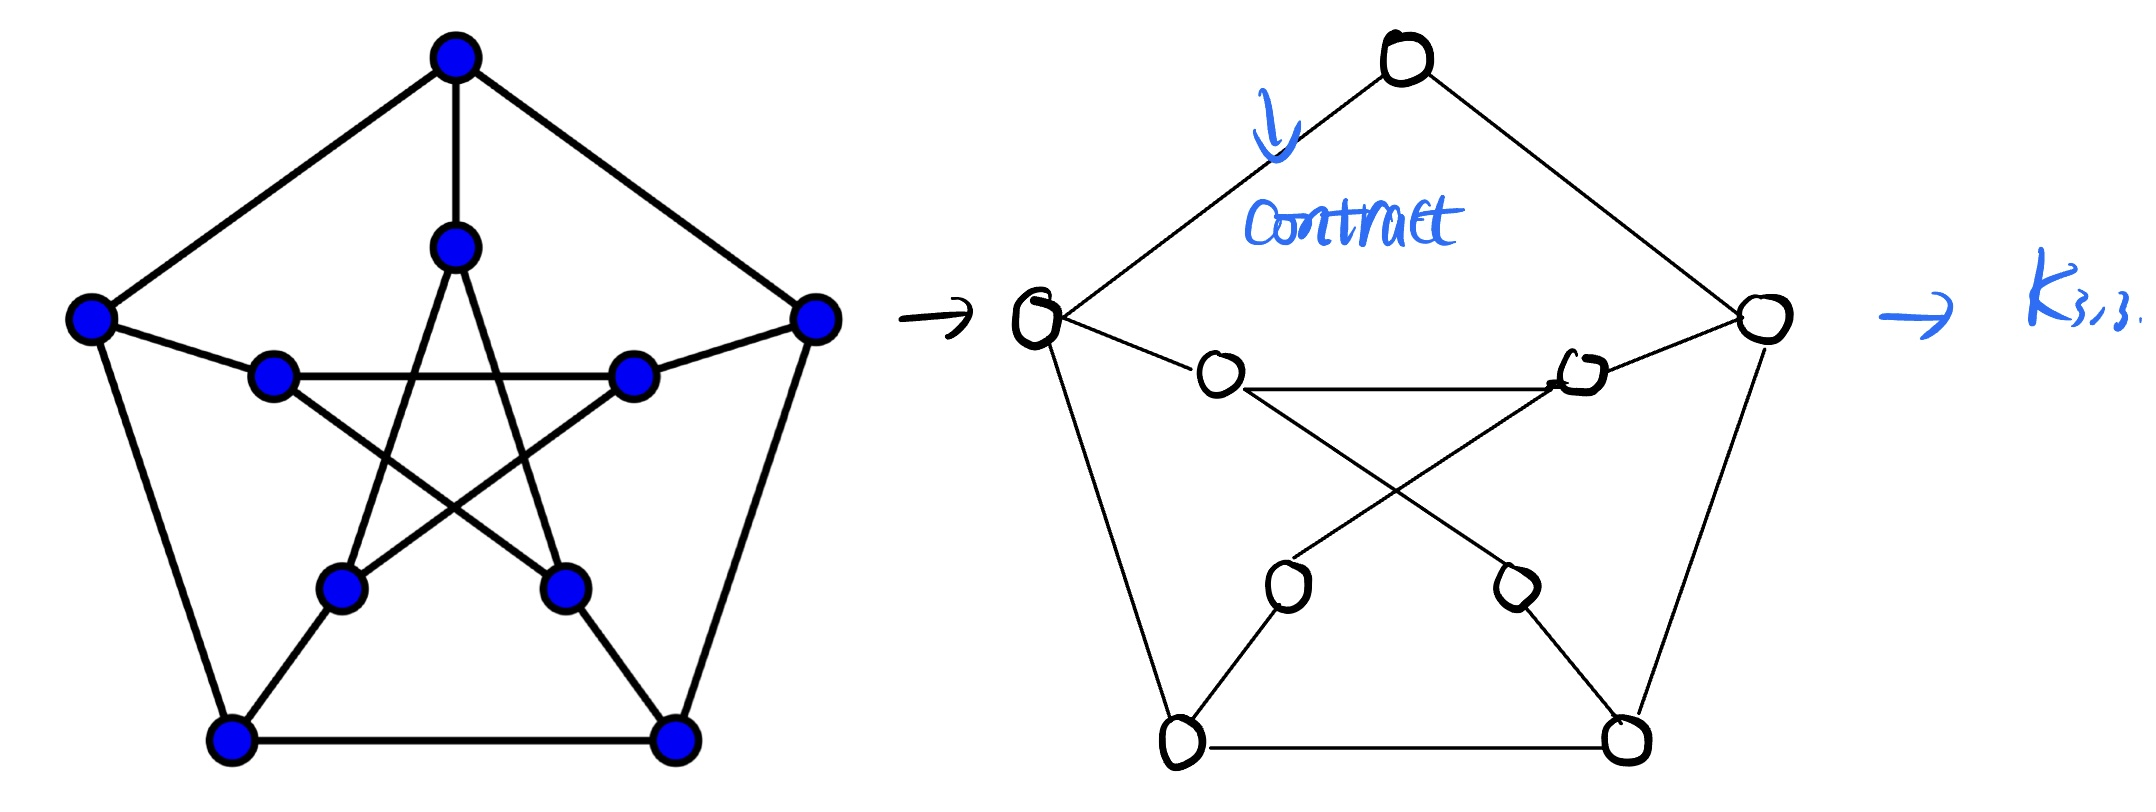
\includegraphics[scale=0.14]{Images/IMG_0305.jpg}
    \caption{Petersen graph is not planar}
\end{figure}

\begin{theorem}
    Let $G$ be a graph. If $G$ is planar, then $\chi(G) \leq4$.
\end{theorem}
\textbf{Remark}:
\begin{itemize}
    \item This was proved via brute force computational methods.
    \item Still open if solvable without extreme case work.
\end{itemize}


\section{Posets}

\begin{definition}
    A \textbf{partially ordered set(poset)} is a pair $\mathbb{P}=(X,P)$ where $X$ is a set and $P \subset X^2$ is a relation that is:
    \begin{itemize}
        \item \underline{Reflexive}: $\forall a \in X. (a,a)\in P$
        \item \underline{Anti-symmetric}: if $a \neq b$ with $(a,b)\in P$, then $(a,b)\notin P$
        \item \underline{Transitive}: if $(a,b)\in P$ and $(b,c)\in P$, then $(a,c) \in P$
    \end{itemize}
\end{definition}
\textbf{Remark}:
\begin{itemize}
    \item Instead writing $(a,b)\in P$, we adopt the notation $a \leq_{\mathbb{P}}$.
    \item Having the subscript is useful. Don't confuse poset orders with more classic orders, though it is acceptable to write $a \leq b$.
\end{itemize}

\begin{definition}
    Given a poset $\mathbb{P}=(X,P)$ and $\mathbb{Q}=(Y,Q)$, an \textbf{embedding} from $\mathbb{P}$ to $\mathbb{Q}$ is an injective map:$f:X \longrightarrow Y$ with the property that $$a \leq_{\mathbb{P}} b \Longleftrightarrow f(a) \leq_{\mathbb{Q}} f(b)$$
    \begin{itemize}
        \item If the embedding is surjective, we call it \textbf{isomorphism}.
        \item If $\mathbb{P}=\mathbb{Q}$, we call it \textbf{automorphism(self isomorphism)}.
    \end{itemize}
\end{definition}

\begin{definition}
    Given a poset $\mathbb{P}=(X,P)$, we call the poset $\mathbb{P}^d=(X,P^d)$ given by $$a \leq_{\mathbb{P}^d} b \Longleftrightarrow b \leq_{\mathbb{P}} b$$
    the \textbf{dual} of $\mathbb{P}$. we say a poset is \textbf{self-dual} if it is isomorphic to its dual.
\end{definition}

\begin{definition}
    Given a poset $\mathbb{P}=(X,P)$ and a point $a \in X$, we say $a$ is \textbf{covered} by a point $b \in X$ if $a <_{\mathbb{P}} b$ and there is no $c$ such that $a <_{\mathbb{P}} c <_{\mathbb{P}} b$.
\end{definition}
\textbf{Remark}:
\begin{itemize}
    \item $b$ is directly above $a$, nothing between, but not necessarily unique.
\end{itemize}

\begin{definition}
    Given a poset $\mathbb{P}=(X,P)$, we call the graph $G=(X,E)$ given by $$\{x,y\}\in E \Longleftrightarrow x \text{ covers }y \text{ or }y \text{ covers }x$$
    the \textbf{cover graph} associated to $\mathbb{P}$.
\end{definition}
\textbf{Remark}:
\begin{itemize}
    \item We can draw the graph in an oriented fashion in which lower vertices correspond to $\leq_{\mathbb{P}}$-smaller elements. We call this depiction a \textbf{Hasse diagram}.
\end{itemize}


\begin{definition}
    Given a poset $\mathbb{P}=(X,P)$, we say two points $a,b \in X$ are \textbf{comparable} if either $$a <_{\mathbb{P}} b \text{ or } b<_{\mathbb{P}} a$$
    If two points are not comparable, we call them \textbf{incomparable}.
\end{definition}


\begin{definition}
    Given a poset $\mathbb{P}$, we say $\mathbb{P}$ is \textbf{linearly ordered} if no two distinct points are incomparable.
\end{definition}
\textbf{Questions}:
\begin{enumerate}
    \item Show that there is only one linear order of size $n$ up to isomorphism.
    \item Show that any linear order is self-dual.
\end{enumerate}


\begin{definition}
    Given a poset $\mathbb{P}$, we call $C \subset X$ a \textbf{chain} if every pari of distinct elements are comparable. 
    We call $A \subset X$ an \textbf{antichain} if every pair of elements in $A$ are incomparable.
\end{definition}


\begin{definition}
    Given a poset $\mathbb{P}$, we define the parameters \textbf{width} and \textbf{height} to denote the size of the largest antichain and chain respectively.
\end{definition}


\begin{theorem}[Spencer]
    Consider the poset $\mathbb{P}=(\mathcal{P}([n]), \subseteq)$, then $$width(\mathbb{P})={n \choose \lfloor \frac{n}{2} \rfloor}$$
\end{theorem}
\begin{proof}
    One can easilly verify $A=\{S \subset \mathcal{P}([n]):|S|=\lfloor \frac{n}{2} \rfloor\}$ is an antichain. (two sets of the same size are comparable iff they are equal.). 
    So $$width(\mathbb{P}) \geq {n \choose \lfloor \frac{n}{2} \rfloor}$$
    Take $A=\{S_1,\cdots,S_w\}$ be a maximal antichain of $\mathbb{P}$, each $S_i \subset [n]$. 
    Consider for each $i \in\{1,\cdots,w\}$, $C_i$ is the set of maximal chains such that $S_i \in C_i$.
    \begin{figure}[ht]
        \centering
        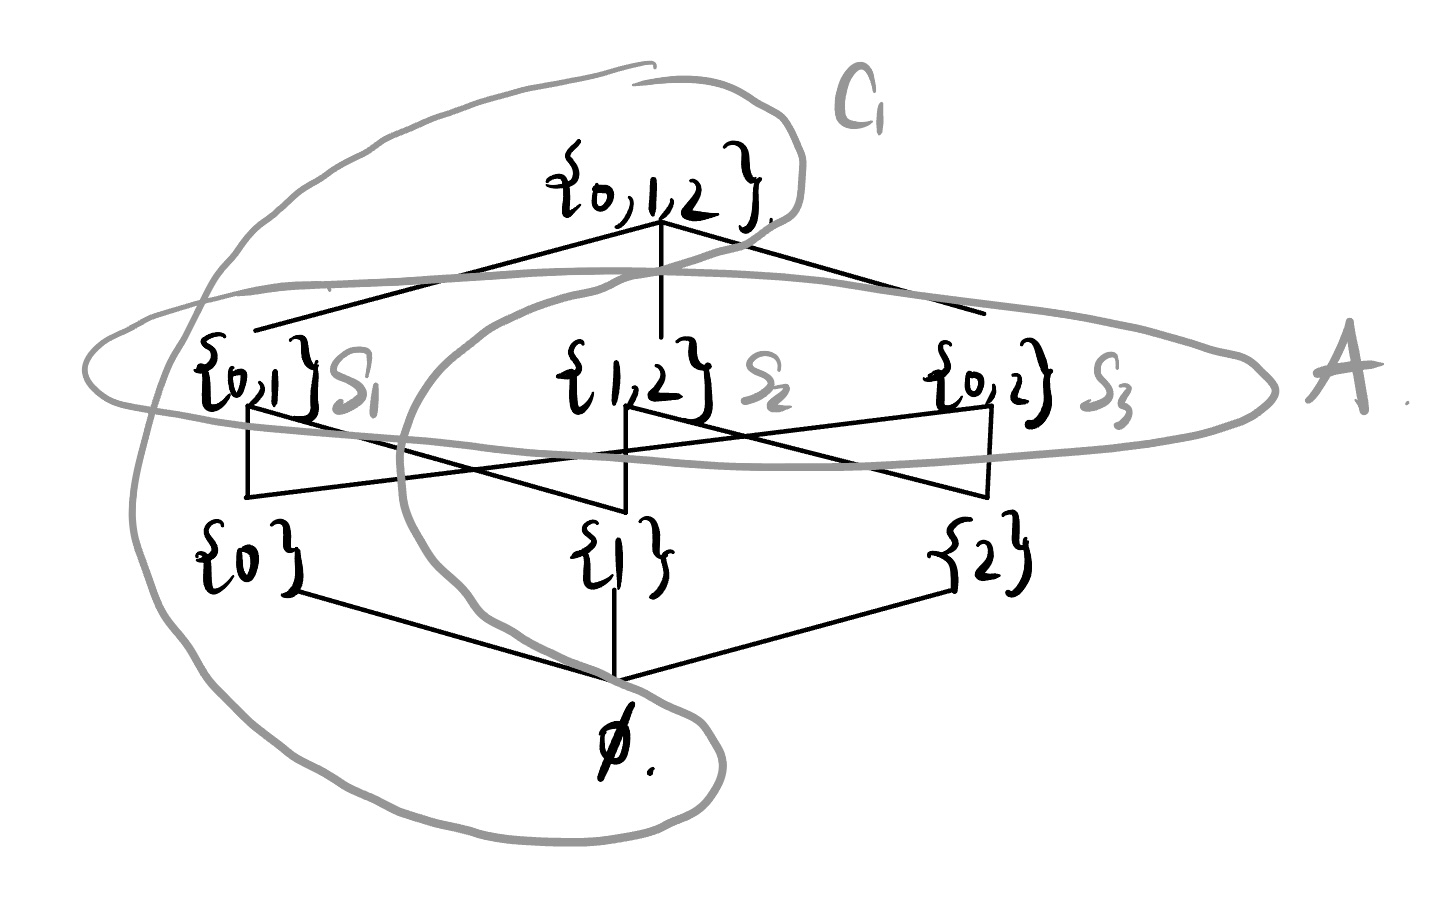
\includegraphics[scale=0.15]{Images/IMG_0306.jpg}
        \caption{A picture discription of the proof}
    \end{figure}
    For any $i$ we have $$|C_i|=|S_i|!(n-|S_i|)!$$ As a maximal chain must be an $\subseteq$-increasing sequence that differs by at most one element per successive cover. 
    There are $(k-|S_i|)!$ many ways to add points successively to $S_i$ and $|S_i|!$ many ways to remove points from $S_i$ successively. 
    Similarly, there are exactly $n!$ many maximal chains.
    \begin{figure}[ht]
        \centering
        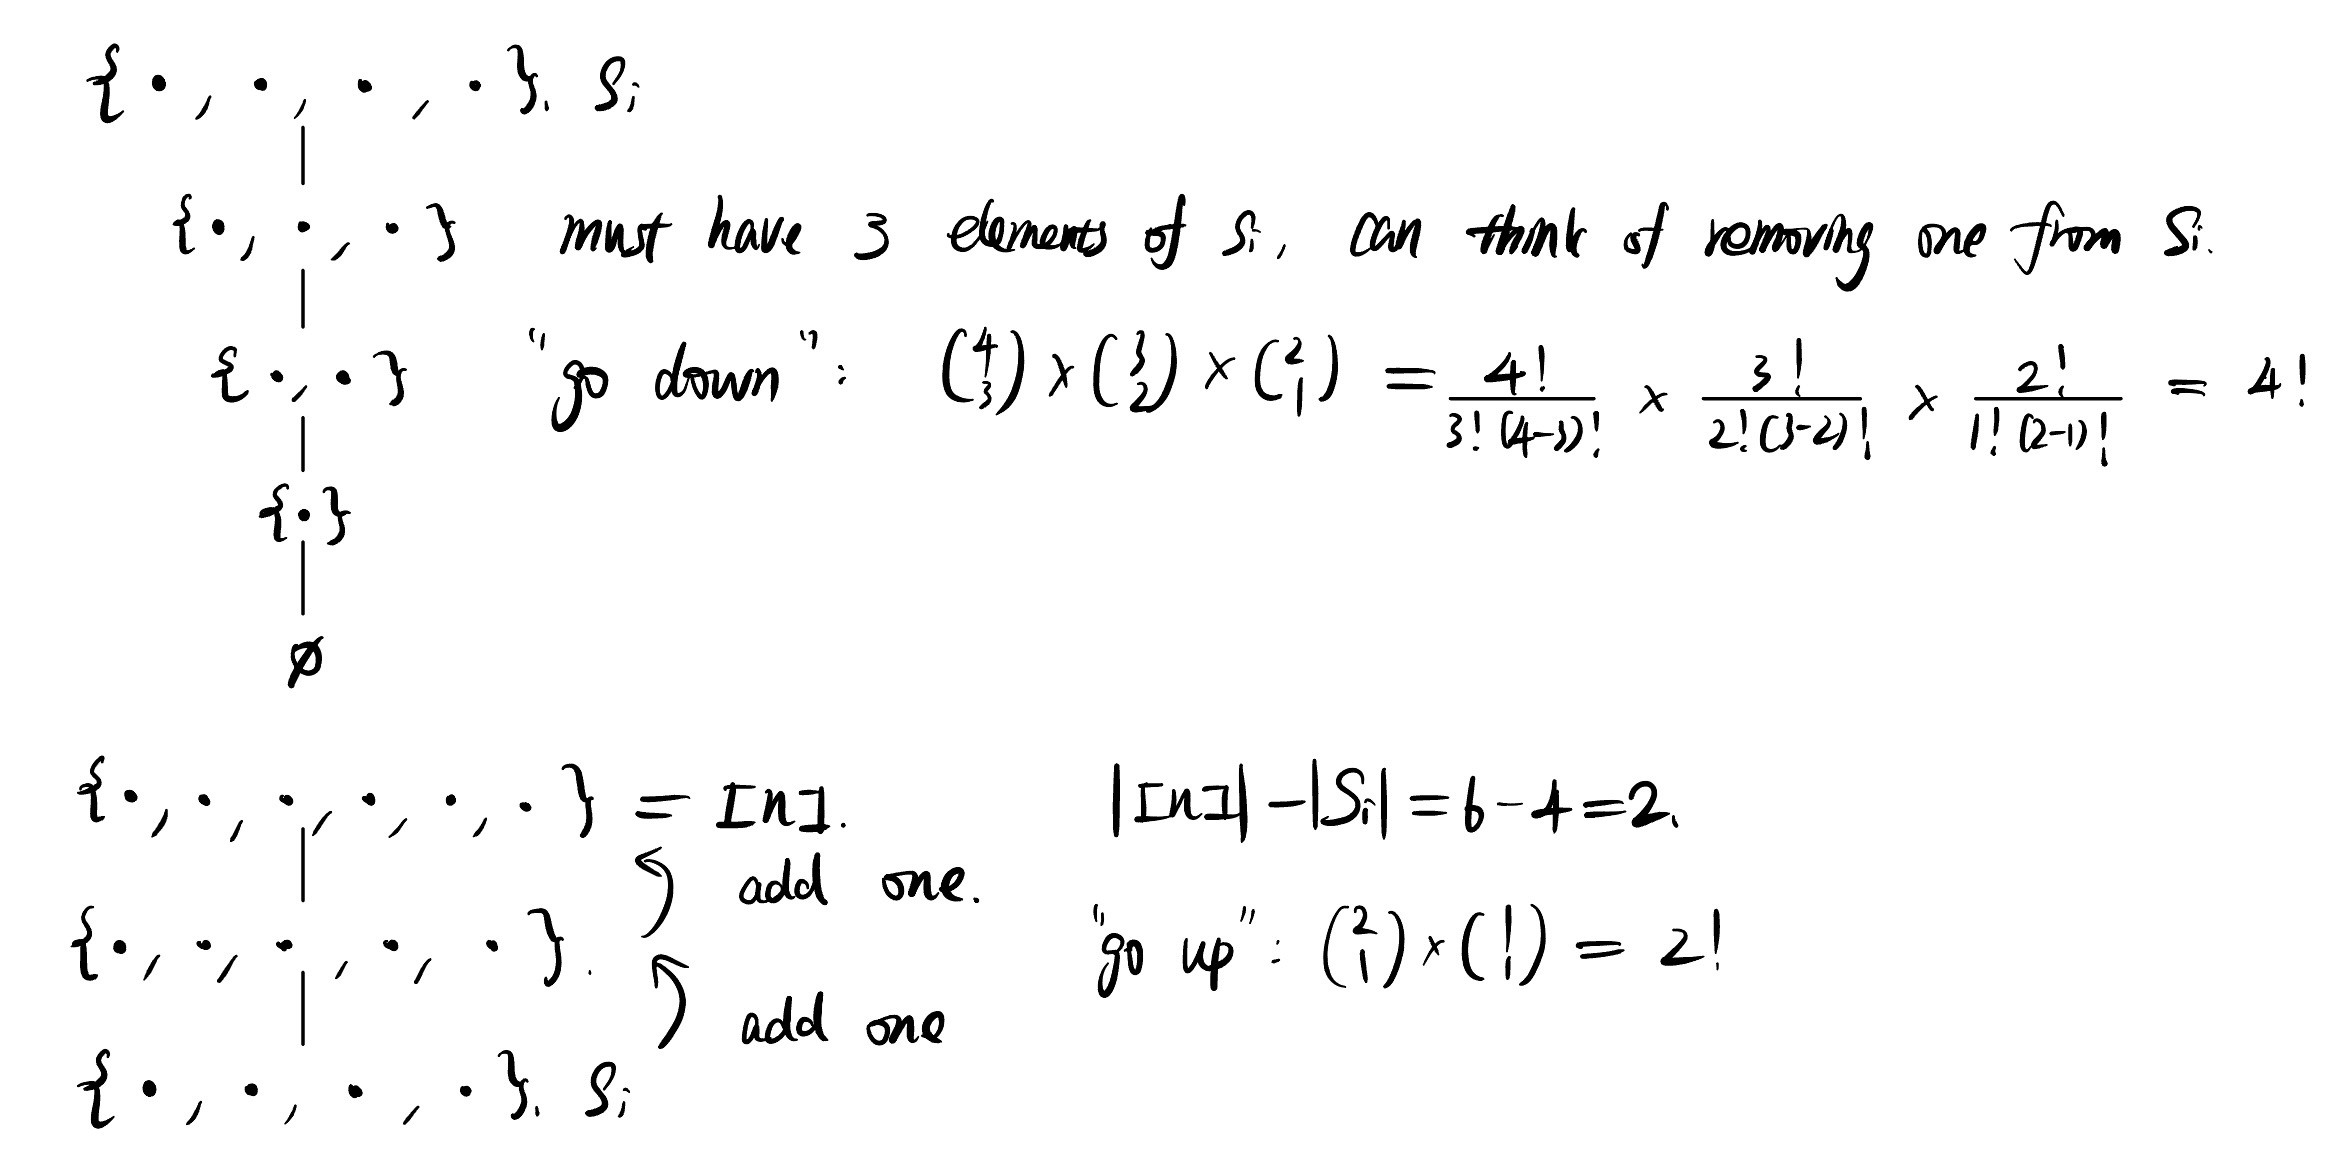
\includegraphics[scale=0.15]{Images/IMG_0307.jpg}
        \caption{A picture discription of the proof}
    \end{figure}
    For any $i \neq j$, $C_i \cap C_j=\{\emptyset,[n]\}$, else there is a chain $C$ with $S_i,S_j \in C$ and hence $S_i$ and $S_j$ are comparable, contradiction. 
    It follows that $$\sum_{i=1}^w|C_i| \leq n!$$ further we have $$\sum_{i=1}^w \frac{|S_i|!(n-|S_i|)!}{n!} \leq 1$$
    hence $$\sum_{i=1}^w \frac{1}{{n \choose |S_i|}} \leq 1$$
    Using that $${n \choose |S_i|} \leq {n \choose \lfloor \frac{n}{2} \rfloor}$$
    we can get the result.
\end{proof}

\begin{theorem}[Mirsky(Dual Dilworth)]
    Let $\mathbb{P}$ be a poset with $height(\mathbb{P})=h$. 
    There is a partition of $X$ into $w$ antichains $A_1,\cdots,A_h$. 
    Moreover, there is optimal in that you cannot cover $\mathbb{P}$ with $<h$ many antichains.
\end{theorem}
\begin{proof}\
    \begin{enumerate}
        \item For each $a \in X$, consider the set $D_a=\{b \in X: b \leq_{\mathbb{P}} a\}$. Let $\mathbb{D}_a=(D_a,P)$.\\
        For each $i \in \{1,\cdots,h\}$, let $A_i=\{a \in X: height(\mathbb{D}_a)=i\}$
        \begin{figure}[ht]
            \centering
            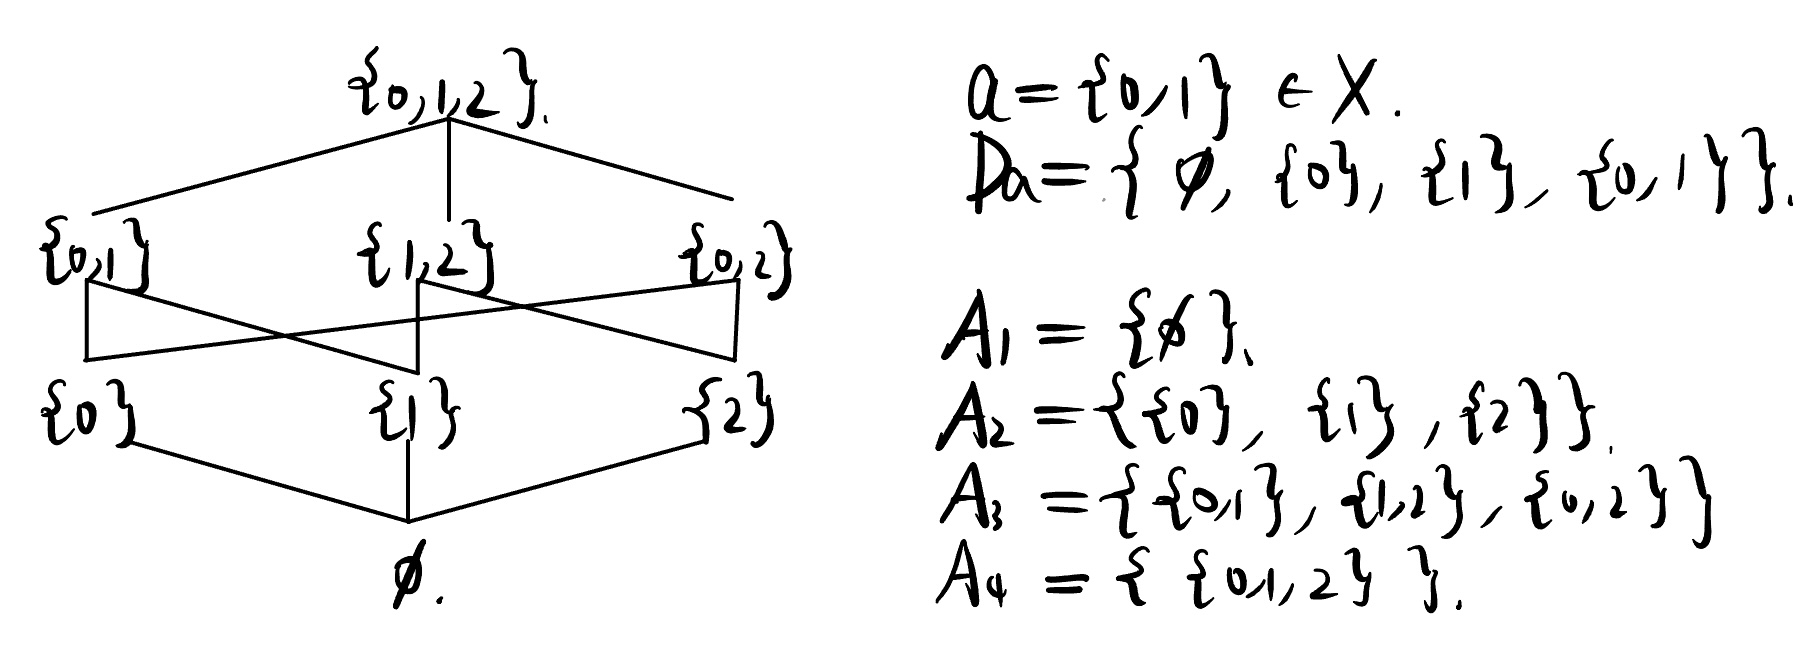
\includegraphics[scale=0.15]{Images/IMG_0310.jpg}
            \caption{A picture discription of the proof}
        \end{figure}
        This forms a proper partition of $X$, as if $|D_a| >h$ for some $a \in X$ would contradict the definition of height. 
        The sets $A_i$ are also antichains. If $height(\mathbb{D}_a)=height(\mathbb{D}_b)$ and $a \in D_b$, then $b \notin D_a$ and $D_a \cup \{b\} \subset D_b$. 
        But then $$height(\mathbb{D}_b) \geq height(\mathbb{D}_a)+1 >height(\mathbb{D}_b)$$
        This is a contradiction.
        \item To see this is optimal, is also by way of contradiction. 
        Suppose we partitioned $X$ into $k$ antichains: $A_1,\cdots,A_k$ for $k < h$. 
        Take a chain $C$ of size $h$ and consider the map $f:C \longrightarrow \{1,\cdots,k\}$ given by $$f(a)=i \Longleftrightarrow a \in A_i$$
        By the Pigeon Hole Principle, there is some $A_i$ that contains two distinct members of $C$, hence the are incomparable. 
        This contradicts to that $C$ is a chain. 
    \end{enumerate}
\end{proof}

\begin{theorem}[Dilworth]
    Let $\mathbb{P}$ be a poset with $width(\mathbb{P})=w$. 
    There is a partition of $X$ into $w$ chains $C_1,\cdots,C_w$. 
    Moreover, there is optimal in that you cannot cover $\mathbb{P}$ with $<w$ many chains.
\end{theorem}
\begin{proof}
    (proceed bt strong induction on $|X|$)\\
    Base case: $|X|=1$. The poset is the one point linear order. So $X$ is a chain itself and we're done.\\
    Inductive step: Take a poset $\mathbb{P}=(X,P)$ with $width(\mathbb{P})=w$ and $hright(\mathbb{P})=h$. 
    Assume the theorem is true for all posets with cardinality $k < |X|$. 
    Let $C=\{x_1,\cdots,x_n\}$ be a maximal chain in $\mathbb{P}$. Consider the subposet $\mathbb{Q}=(X \setminus C, P \cap (X \setminus C)^2)$. 
    Note that $width(\mathbb{Q}) \leq width(\mathbb{P})$. 
    \begin{enumerate}
        \item Case1: $width(\mathbb{Q}) < width(\mathbb{P})$.\\ 
        We claim that $$width(\mathbb{Q})=w-1$$
        By assumption, we have $width(\mathbb{Q})=w' \leq w-1$. Since $height(\mathbb{P})=h$,
        by Mirsky's theorem, we have minimal number of antichains: $A_1,\cdots,A_{h'}$. So $w = max\{|A_1|,\cdots,|A_n|\}$. 
        Since $height(\mathbb{q})=h' \leq h$, by Mirsky's theorem, we have minimal number of antichains:$B_1,\cdots,B_{h'}$. So $w'=max\{|B_1|,\cdots,|B_{h'}\}$. \
        We removed a chain $C$ from $\mathbb{P}$. Can use Pigeon Hole Principle to show that: for each $A_i$, we removed one element. 
        The new $A_i'$s are also antichains which forms a partition for $\mathbb{Q}$. 
        By definitionof width, $$w' \geq max\{|A_1|-1,\cdots,|A_n|-1\}=w-1$$
        Hence $w'=w-1$.\\
        Apply the induction hypothesis to $\mathbb{Q}$, can cover it with $C_1,\cdots,C_{w-1}$ chains. Then $C_1,\cdots,C_{w-1},C$ forms a cover of $\mathbb{P}$ with $w$many chains.
        \item Case2: $width(\mathbb{Q})=width(\mathbb{P})$.\\
        \begin{figure}[ht]
            \centering
            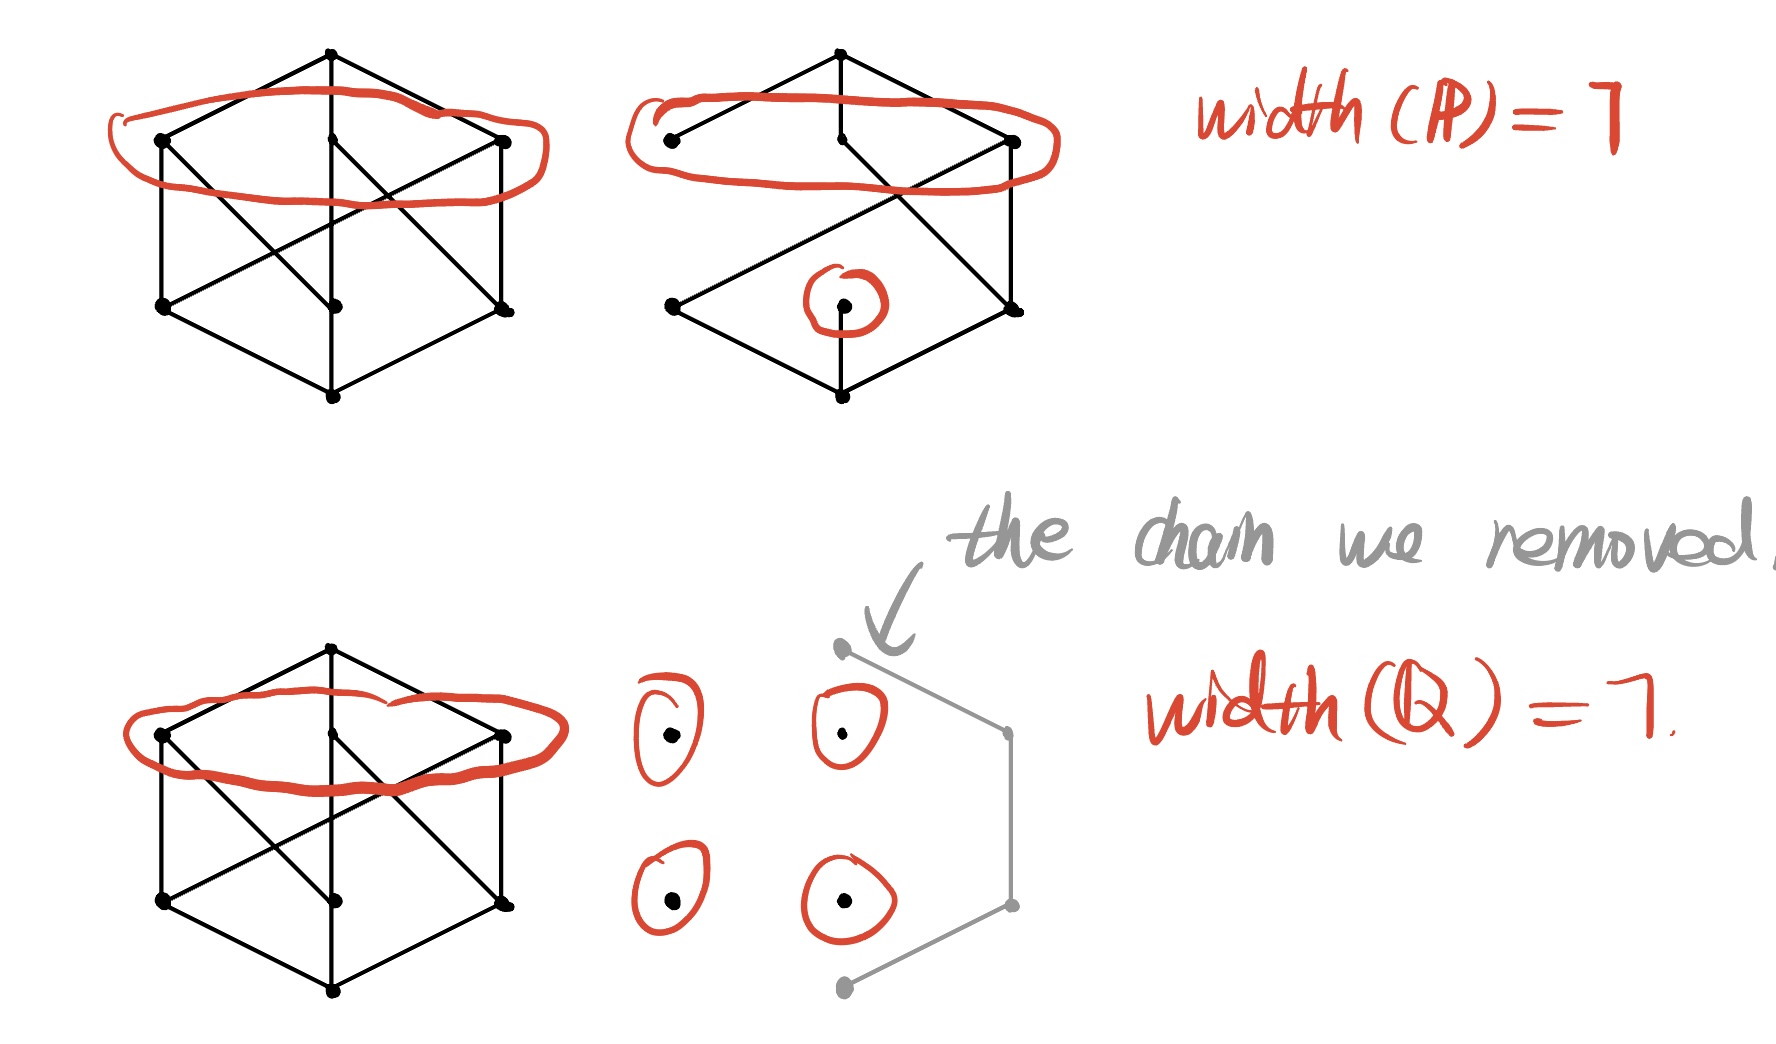
\includegraphics[scale=0.15]{Images/IMG_0308.jpg}
            \caption{A picture discription of the proof}
        \end{figure}
        Take an antichain $A=\{a_1,\cdots,a_w\} \subset X \setminus C$.\\ 
        Note, for any $a_i \in A$, $a_i$ is notbigger than $x_n$(i.e.not $x_n <_{\mathbb{P}} a_i$)else we'd contradict maximality of $C$. Define:
        \begin{itemize}
            \item $\mathbb{P}^-=\{x \in X: \exists a \in A. x \leq_{\mathbb{P}} a\}$
            \item $\mathbb{P}^+=\{x \in X: \exists a \in A. a \leq_{\mathbb{P}} x\}$
        \end{itemize}
        \begin{figure}[ht]
            \centering
            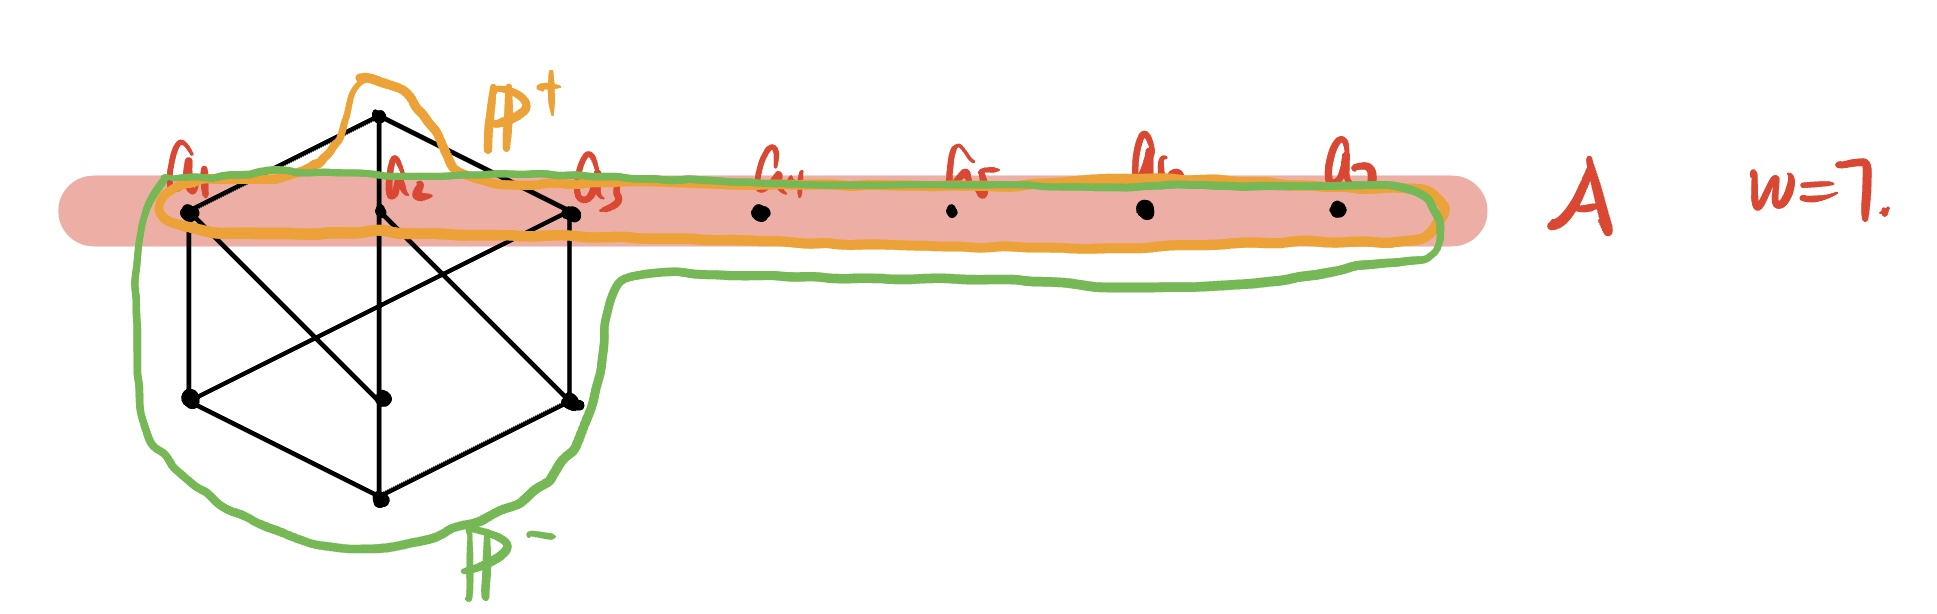
\includegraphics[scale=0.14]{Images/IMG_0309.jpg}
            \caption{A picture discription of the proof}
        \end{figure}
        Apply the induction hypothesis on $\mathbb{P}^+$ and $\mathbb{P}^-$. 
        This gives us chains $C_1^-,\cdots,C_w^-$ and $C_1^+,\cdots,C_w^+$ covering $\mathbb{P}^+$ and $\mathbb{P}^-$ respectively. 
        We may do also assume without loss of generality, $a_i \in C_i^+ \cap C_i^-$. 
        Set $C_i=C_i^+ \cap C_i^-$. This forms a family of $w$ chains cover the poset $\mathbb{P}$.
    \end{enumerate}
\end{proof}


\begin{theorem}[Erdös-Szekeres]
    Let $\{x_i: i \in [rs+1]\}$ be a family of $rs+1$ distinct real numbers. 
    There is a strictly increasing subsequence of length $r+1$ or a strictly decreasing subsequence of length $s+1$.
\end{theorem}
\begin{proof}
    Consider the poset $\mathbb{P}=(X,P)$ where $X=\{(i,x_i):i \in [re+1]\}$ and 
    $$(i,x_i) \leq_{\mathbb{P}} (j,x_j) \Longleftrightarrow i \leq j \text{ and } x_i \leq x_j$$
    If $height(\mathbb{P}) \geq r+1$, then we're done. As a maximal chain codes a strictly increasing subsequence $x_{n_k}$ of size $\geq r+1$. 
    Suppose $height(\mathbb{P}) \leq r$. Using Dilworth's theorem, can find a cover for $\mathbb{P}$ into $w=width(\mathbb{P})$ many chains $C_1,\cdots,C_w$. 
    Note that $|C_i| \leq r$, so $w \geq s+1$. Else we can cover $X$ with $\cup_{i=1}^wC_i$, which has at most $rs$ many points, contradiction. 
    It follows that there is an antichain $A=\{(n_1,x_{n_1}),\cdots,(n_{s+1},x_{n_{s+1}})\}$ where we assume that $$i<j \Longrightarrow n_i<n_j$$
    By the way we've defined $\mathbb{P}$. If $n_i<n_j$, then $x_{n_i}>x_{n_j}$. Else $(n_i,x_{n_i}) \leq_{\mathbb{P}} (n_j,x_{n_j})$, contradicting that $A$ is an antichain. 
    It follows that $x_{n_i}$ is a decreasing subsequence of size at least $s+1$.
\end{proof}
\textbf{My question}:
\begin{itemize}
    \item What is the relation between this and Bolzano-Weierstrass theorem? This looks like a finite version of Bolzano-Weierstrass theorem.
\end{itemize}

\begin{definition}
    Let $\mathbb{P}=(X,P)$ be a poset. A \textbf{linear extension} of $\mathbb{P}$ is a linear order $\mathbb{L}=(X,L)$ where $P \subset L$.i.e. a linear ordering $\leq_{\mathbb{L}}$ on $X$ with property $$a \leq_{\mathbb{P}} b \Longrightarrow a \leq_{\mathbb{L}} b$$
\end{definition}
\begin{proof}
    We do this recursively by creating a sequence of extensions $\mathbb{P}_i=(X,P-i)$ of $\mathbb{P}$, where at the terminal stage we have a linear order. 
    Suppose we're at stage $i$ and have a poset $\mathbb{P}_i$. 
    If $\mathbb{P}_i$ is not a linear order, there must be two points $a,b \in X$ that are not $\mathbb{P}_i$-comparable. 
    Construct $\mathbb{P}_{i+1}$ by setting:
    $$P_{i+1} = P_i \cup \{(a,b)\}\cup \{(x,y)\in X^2: x \leq_{\mathbb{P}_i} a \text{ and } b \leq_{\mathbb{P}_i} y\}$$
    One should confirm that $\mathbb{P}_{i+1}$ is indeed transitive. 
    Eventually this process must halt, else we'd have found an infinite sequence of pairs $(a_i,b_i)\in X^2$ that are incomparable.
\end{proof}
\textbf{Remark}:
\begin{itemize}
    \item In computer science, a topological sort or topological ordering of a directed graph is a linear ordering of its vertices.
\end{itemize}
\chapter{Generating Functions}

In mathematics, we have the discrete world such as natural numbers, graphs. And also the continuous world such as analysis. 
Luckily we are going to introduce a bridge between the two worlds, which is generating function. 

\section{Ordinary Generating Functions}
\begin{definition}
    Given a sequence of real numbers $a_n(n \geq 0)$. 
    We let the function $F(x)=\sum_{n=0}^{\infty}a_nx^n$ denote the \textbf{ordinary generating function} associated to $a_n$.
\end{definition}
\textbf{Remark}
\begin{itemize}
    \item The above function that we defined may not be convergent for any x.
    \item We will just use these functions as a book keeping system.
\end{itemize}

\begin{theorem}[The geometric series]
    Consider the sequence $a_n=1$ for all integers $n \geq 0$. 
    The associated generating function is $F(x)=\frac{1}{1-x}$,
\end{theorem}
\begin{proof}
    It suffices to show $(1-x)F(x)=1$.
    \begin{equation}
        \begin{split}
            (1-x)F(x) &= (1-x)\sum_{n=0}^{\infty}x^n\\
            &= \sum_{n=0}^{\infty}x^n - x \sum_{n=0}^{\infty}x^n\\
            &= \sum_{n=0}^{\infty}x^n - \sum_{n=0}^{\infty}x^{n+1}\\
            &= \sum_{n=0}^{\infty}x^n - \sum_{n=1}^{\infty}x^n\\
            &= 1
        \end{split}
    \end{equation}
\end{proof}

\begin{theorem}[The finite geometric series]
    Consider the sequence 
    \begin{equation}
        \begin{cases}
            a_n=1& \text{for all integers $0 \leq n \leq k$}\\
            a_n=0& \text{for all integers $n>k$}
        \end{cases}
    \end{equation}
    Then the associated generating function is $F(x)=\frac{1-x^{k+1}}{1-x}$
\end{theorem}
\textbf{Remark}
\begin{itemize}
    \item Writing in this way mimics inclusion-exclusion.
\end{itemize}
\begin{proof}
    \begin{equation}
        \begin{split}
            (1-x)F(x) &= (1-x)\sum_{n=0}^{k}x^n\\
            &= \sum_{n=0}^{k}x^n - x \sum_{n=0}^{k}x^n\\
            &= \sum_{n=0}^{k}x^n - \sum_{n=0}^{k}x^{n+1}\\
            &= \sum_{n=0}^{k}x^n - \sum_{n=1}^{k+1}x^n\\
            &= 1-x^{k+1}
        \end{split}
    \end{equation}
\end{proof}

\noindent \textbf{Questions} Find the generating functions.
\begin{enumerate}
    \item $\forall n \geq 0. a_n=2$
    \item $\forall n \geq 0. a_n=2^n$
    \item $a_n=1$ for $n \geq 5$ and 0 otherwise.
    \item $a_n=1$ for all $n \geq 0$ and even. $a_n=0$ otherwise.
    \item $\forall n \geq 0. a_n=2^n+1$
\end{enumerate}
\textbf{Answers}
\begin{enumerate}
    \item $F(x)=\sum_{n=0}^{\infty}a_nx^n=\sum_{n=0}^{\infty}2x^n=2\sum_{n=0}^{\infty}x^n=\frac{2}{1-x}$
    \item $F(x)=\sum_{n=0}^{\infty}a_nx^n=\sum_{n=0}^{\infty}2^nx^n=\sum_{n=0}^{\infty}(2x)^n=\frac{1}{1-2x}$
    \item define $c_n, b_n$ as below: 
    \begin{equation}
        \forall n \geq 0. c_n=1
    \end{equation} 
    \begin{equation}
        b_n = 
        \begin{cases}
            1& \text{$n<5$}\\
            0& \text{$n \geq 5$}
        \end{cases}
    \end{equation} 
    The we have $a_n=c_n-b_n$. 
    \begin{equation}
        \begin{split}
            F(x) &= \sum_{n=0}^{\infty}(c_n-b_n)x^n\\
            &= \sum_{n=0}^{\infty}c_nx^n - \sum_{n=0}^{\infty}b_nx^n\\
            &= \sum_{n=0}^{\infty}x^n - \sum_{n=0}^{4}x^n\\
            &= \frac{1}{1-x}- \frac{1-x^5}{1-x}\\
            &= \frac{x^5}{1-x}
        \end{split}
    \end{equation}
    \item \begin{equation}
        \begin{split}
            F(x) &= \sum_{n=0}^{\infty}a_nx^n\\
            &= \sum_{n=0}^{\infty}x^{2n}\\
            &= \frac{1}{1-x^2}
        \end{split}
    \end{equation}
    \item We will use linearity to calculate this.
\end{enumerate}

\begin{theorem}[Linearity]
    Take two sequences $a_n$ and $b_n$. 
    Let $F(x)$ and $G(x)$ be the associated (ordinary) generating functions respectively. 
    Let $c_n=a_n+b_n$. Then the (ordinary) generating function associated to $c_n$ is the function $F(x)+G(x)$.
\end{theorem}
\begin{proof}
    \begin{equation}
        \begin{split}
            F(x)+G(x) &= \sum_{n=0}^{\infty}a_nx^n + \sum_{n=0}^{\infty}b_nx^n\\
            &= \sum_{n=0}^{\infty}(a_nx^n+b_nx^n)\\
            &= \sum_{n=0}^{\infty}(a_n+b_n)x^n\\
            &= \sum_{n=0}^{\infty}c_nx^n\\
        \end{split}
    \end{equation}
\end{proof}

\begin{theorem}[Derivatives]
    Let $a_n$ be a sequence and let $b_{n-1}=na_n$ for $n \geq 1$. 
    If $F(x)$ is the generating function associated to $a_n$. Then $F'(x)$ is the generating function associated to $b_n$.
\end{theorem}
\begin{proof}
    Since we have $F(x)$ and we know that the derivative is linear, we can take it term by term.
    \begin{equation}
        \begin{split}
            F'(x) &= \frac{dF(x)}{dx}\\
            &= \sum_{n=0}^{\infty}na_nx^{n-1}\\
            &= \sum_{n=1}^{\infty}na_nx^{n-1}\\
            &= \sum_{n=1}^{\infty}b_{n-1}x^{n-1}\\
            &= \sum_{n=0}^{\infty}b_nx^n
        \end{split}
    \end{equation}
\end{proof}

\begin{theorem}[Multiplication]
    Let $F(x)=\sum_{n=0}^{\infty}a_nx^n$ and $G(x)=\sum_{n=0}^{\infty}b_nx^n$. 
    Then $$H(x)=F(x)G(x)= \sum_{n=0}^{\infty}c_nx^n$$ where 
    $$c_n=\sum_{m+i=n}a_mb_i=\sum_{k=0}^na_{n-k}b_k$$
\end{theorem}

\begin{theorem}[Multiple products]
    Let $F_1(x), \cdots ,F_m(x)$ be generating functions with $F_i(x)=\sum_{n=0}^{\infty}a_{n,i}x^n$. 
    Then $$F_1(x) \times \cdots \times F_m(x)=\sum_{n=0}^{\infty}c_nx^n$$ 
    where $$c_n=\sum_{e_1+ \cdots +e_m=n}a_{e_1,1}\times \cdots \times a_{e_m,m}$$
\end{theorem}

\noindent \textbf{Computation practice}
\begin{enumerate}
    \item $\frac{1}{(1-x)^2}$
    \item $\frac{1}{(1-x)^3}$
    \item $e^x$
    \item $\frac{e^x}{1+x}$
    \item $\frac{1+x+x^2}{(1-x)^{50}}$
    \item Find the number of integer solutions to the equation $e_1+e_2+e_3=25$ with $e_i \geq 0$ for all $i \in \{1,2,3\}$. $e_1$ even. $e_3 \leq 2$.
\end{enumerate}
\textbf{Answers}
\begin{enumerate}
    \item \begin{equation}
        \begin{split}
            \frac{1}{(1-x)^2} &= \frac{1}{1-x}\frac{1}{1-x}\\
            &= (1+x+x^2+x^3+ \cdots)(1+x+x^2+x^3+ \cdots)\\
            &= \sum_{n=0}^{\infty}c_nx^n
        \end{split}
    \end{equation}
    We can now use the Multiplication rule and stars and bars to calculate $c_n$.
    $$c_n=\sum_{e_1+e_2=n}1 \times 1={n+(2-1) \choose 2-1}={n+1 \choose 1}=n+1$$
    \item Similar to the last question $$c_n = \sum_{e_1+e_2+e_3}1 \times 1 \times 1={n+2 \choose 2}$$
    \item Using taylor expansion $$e^x=\sum_{n=0}^{\infty}\frac{1}{n!}x^n$$
    \item \begin{equation}
        \begin{split}
            \frac{e^x}{1+x} &= (\sum_{n=0}^{\infty}\frac{1}{n!}x^n)\times (\sum_{n=0}^{\infty}(-x)^n)\\
            &= \sum_{n=0}^{\infty}c_nx^n
        \end{split}
    \end{equation}
    where $$c_n=\sum_{e_1+e_2=n}\frac{1}{e_1!}(-1)^{e_2}=\sum_{k=0}^n\frac{1}{k!}(-1)^{n-k}$$
    \item \begin{equation}
        \begin{split}
            \frac{1+x+x^2}{(1-x)^{50}} &= \frac{1}{(1-x)^{50}} + \frac{x}{(1-x)^{50}} + \frac{x^2}{(1-x)^{50}}\\
            &= {n+49 \choose 49} + {n+48 \choose 49} + {n+47 \choose 49}
        \end{split}
    \end{equation}
    \item Let us first compute the generationg function $F(x)=\sum_{n=0}^{\infty}a_nx^n$ associated to the solutions $\{a_n\}$. 
    $\{a_n\}$ is a sequence, where $a_n$ = number of solutions of $e_1+e_2+e_3=n$.
    \begin{itemize}
        \item Solutions of $e_1$: $S_{e_1}=\{0,2,4,6, \cdots\}$
        \item Solutions of $e_2$: $S_{e_2}=\{0,1,2,3, \cdots\}$
        \item Solutions of $e_3$: $S_{e_3}=\{0,1,2\}$
    \end{itemize}
    Then we only need to show $a_{25}$. i.e. choose one of $S_{e_1},S_{e_2},S_{e_3}$ to make 25. 
    This is equivalent to find the coefficient of $x^{25}$ for the function below.
    $$(x^0+x^2+x^4+ \cdots)(x^0+x^1+x^2+\cdots)(x^0+x^1+x^2)=\frac{1}{1-x^2}\frac{1}{1-x}\frac{1-x^3}{1-x}$$
\end{enumerate}

\begin{definition}
    Given a power series $f(x)=\sum_{n=0}^{\infty}a_nx^n$, 
    we often write the shorthand $[x^n](f(x))=a_n$ instead of saying the n-th coefficient.
\end{definition}
\textbf{Remark}
\begin{itemize}
    \item We can view this notation as a function where the input is the function $f$ and the output is the coefficient.
    \item $[x^n](f(x)+g(x))=[x^n](f(x))+[x^n](g(x))$
\end{itemize}

\begin{theorem}
    $\forall p \in \N \cup\{0\}. [x^n]((1+x)^p)={p \choose n}$
\end{theorem}
\begin{proof}
    Recall the Binomial theorem and use the definition above.
\end{proof}

\section{Newton's Binomial Theorem}

\begin{theorem}[Newton's Binomial Theorem]
    For every \underline{non-zero real number} p. 
    We have the power series expansion of $(1+x)^p$
    $$\sum_{k=0}^{\infty}\frac{f^{(k)}(0)}{k!}x^k$$
    We let ${p \choose n}$ denote the unique n-th coefficient in the power series.
\end{theorem}
\textbf{Remark}
\begin{itemize}
    \item Normally, one can also define $P(p,n)={p \choose n}n!$
\end{itemize}

\begin{lemma}
    For all real p for which it is defined. we have ${p \choose 0}=1$.
\end{lemma}
\begin{proof}
    ${p \choose 0}=\frac{f^{(0)}(0)}{0!}=\frac{f(0)}{1}=(1+0)^p=1$
\end{proof}

\begin{lemma}
    For all real p for which it is defined and $n \in \N$.
    $${p \choose n}=\frac{p}{n}{p-1 \choose n-1}$$
\end{lemma}
\begin{proof}:
    \begin{itemize}
        \item For $p \in \N$, it is trivial. $${p \choose n}=\frac{p!}{n!(p-n)!}=\frac{p}{n}\frac{(p-1)!}{(n-1)!(p-n)!}$$
        \item We focus on $p \notin \N$. By Newton's Binomial Theorem we have $$(1+x)^p=\sum_{k=0}^{\infty}{p \choose n}x^n$$
        Let us take the derivative for both sides.
        \begin{equation}
            \begin{split}
                p(1+x)^{p-1} &= \sum_{n=0}^{\infty}{p \choose n}nx^{n-1}\\
                (1+x)^{p-1} &= \sum_{n=0}^{\infty}\frac{n}{p}{p \choose n}x^{n-1}
            \end{split}
        \end{equation}
        Find the coefficient for $x^{n-1}$ for both sides
        \begin{equation}
            \begin{split}
                [x^{n-1}]((1+x)^{p-1}) &= {p-1 \choose n-1}\\
                [x^{n-1}](\sum_{n=0}^{\infty}\frac{n}{p}{p \choose n}x^{n-1}) &= \frac{n}{p}{p \choose n}
            \end{split}
        \end{equation}
        Hence we have $${p-1 \choose n-1}= \frac{n}{p}{p \choose n}$$
        Therefore, $${p \choose n}= \frac{p}{n}{p-1 \choose n-1}$$
    \end{itemize}
\end{proof}

\noindent \textbf{Examples}
Using the above theorems and lemmas, we can efficiently compute some fractinal binomial coefficients.
\begin{enumerate}
    \item ${-5 \choose 3}$
    \item ${\frac{1}{2} \choose 3}$
\end{enumerate}
\textbf{Answers}
\begin{enumerate}
    \item \begin{equation}
        \begin{split}
            {-5 \choose 3} &= \frac{-5}{3}\cdot{-6 \choose 2}\\
            &= \frac{-5}{3}\cdot\frac{-6}{2}\cdot{-7 \choose 1}\\
            &= \frac{-5}{3}\cdot\frac{-6}{2}\cdot\frac{-7}{1}{-8 \choose 0}
        \end{split}
    \end{equation}
    \item \begin{equation}
        \begin{split}
            {\frac{1}{2} \choose 3} &= \frac{\frac{1}{2}}{3} \cdot {-\frac{1}{2} \choose 2}\\
            &= \frac{\frac{1}{2}}{3}\cdot\frac{-\frac{1}{2}}{2}\cdot{-\frac{3}{2} \choose 1}\\
            &= \frac{\frac{1}{2}}{3}\cdot\frac{-\frac{1}{2}}{2}\cdot\frac{-\frac{3}{2}}{1}\cdot{-\frac{5}{2} \choose 0}
        \end{split}
    \end{equation}
\end{enumerate}

\begin{theorem}
    For $p<0$ $${p \choose n}= (-1)^n{-p+n-1 \choose n}$$
\end{theorem}
\begin{proof}
    By induction.
\end{proof}

\begin{corollary}
    For $p>0$ $$\frac{1}{(1+x)^p}=\sum_{n=0}^{\infty}(-1)^n{p+n-1 \choose n}x^n$$
\end{corollary}

\begin{lemma}
    $$(1-4x)^{-\frac{1}{2}}=\sum_{n=0}^{\infty}{2n \choose n}x^n$$
\end{lemma}
\begin{proof}
    By Newton's Binomial Theorem we have: $$(1-4x)^{-\frac{1}{2}}=\sum_{n=0}^{\infty}{-\frac{1}{2} \choose n}(-2x)^n$$
    So it suffices to show that $${-\frac{1}{2} \choose n}(-4)^n={2n \choose n}$$
    We finish the proof by showing:
    \begin{equation}
        \begin{split}
            {-\frac{1}{2} \choose n}(-4)^n &= (-1)^n \cdot 2^{2n} \cdot {-\frac{1}{2} \choose n}\\
            &= (-1)^n \cdot 2^{2n} \cdot \frac{-\frac{1}{2}}{n}{-\frac{1}{2}-1 \choose n-1}\\
            &= (-1)^n \cdot 2^{2n} \cdot \frac{-\frac{1}{2}}{n} \cdot \frac{-\frac{1}{2}-1}{n-1} \cdot {-\frac{1}{2}-1 \choose n-1}\\
            &= (-1)^n \cdot 2^{2n} \cdot \frac{-\frac{1}{2}(-\frac{1}{2}-1) \cdots (-\frac{1}{2}-(n-1))}{n(n-1) \cdots 1}\\
            &= (-1)^n \cdot 2^{2n} \cdot \frac{(-\frac{1}{2})(-\frac{3}{2}) \cdots (-\frac{1-2n}{2})}{n!}\\
            &= (-1)^n \cdot 2^{2n} \cdot \frac{(-1)(-3) \cdots (1-2n)}{2^n \cdot n!}\\
            &= (-1)^n \cdot 2^{2n} \cdot \frac{(-1)^n(1 \times 3 \times \cdots \times (2n-1))}{2^n \cdot n!}\\
            &= (-1)^n \cdot 2^{2n} \cdot \frac{(-1)^n}{2^n} \cdot \frac{1 \times 2 \times3 \times 4 \times \cdots \times (2n-1) \times 2n}{n!} \cdot \frac{1}{2 \times 4 \times 6 \times \cdots \times 2n}\\
            &= 2^n \cdot \frac{(2n)!}{n!} \cdot \frac{1}{2^n \cdot n!}\\
            &= \frac{(2n)!}{n!(2n-n)!}\\
            &= {2n \choose n}
        \end{split}
    \end{equation}
\end{proof}

\section{Partition of integers}

We have learnt some properties of integers from elimentary school. This times we will use the ordinary generating functions as a powerful method to find some interesting facts.

\begin{definition}
    A \textbf{partition of an integer $n$} is a multiset $P$. 
    (a set that is allowed to have the same element multiple times) 
    with the property that $$\sum_{i \in P}i=n \text{ with } i>0$$
\end{definition}
\textbf{Remark}
\begin{itemize}
    \item The key idea here is a partition is a splitting of an integer into pieces, 
    where order does not matter, contrary to distribution problems.
    \item $\{1,2,1,1\}=\{2,1,1,1\}$ sometimes we like decending order.
\end{itemize}
\textbf{Example:} partitions of the integer 5:
$$\{5\},\{4,1\},\{3,2\},\{2,2,1\},\{3,1,1\},\{2,1,1,1\},\{1,1,1,1,1\}$$

There is a better way to view partitions:
\begin{definition}
    A \textbf{partition of an integer $n$} is an infinite string of integers $e_i \geq 0$ 
    indexed by $i \in \N$ with the property that $$\sum_{i=1}^{\infty}i \cdot e_i=n$$
\end{definition}
\textbf{Remark:}
\begin{itemize}
    \item These strings count the frequency of a piece of size $e_i$. i.e. $i$ repeated $e_i$ times.
    \item This is more formal than multisets and helps you see the next theorems more clearly.
    \item We can see some similar constructions in some diagonalization proofs.
\end{itemize}
\textbf{Example:} Still consider the partition of the integer 5:
\begin{itemize}
    \item $\{5\}: 00001000 \cdots $
    \item $\{4,1\}: 10010000 \cdots $
    \item $\{3,1,1\}: 20100000 \cdots $
\end{itemize}

\begin{definition}
    We use $p_n$ to denote the number of partitions of the integer n.
\end{definition}

\begin{theorem}
    Let $P(x)=\sum_{n=0}^{\infty}p_nx^n$. 
    We can then express $P(x)$ as the infinite product $$P(x)=\prod_{n=1}^{\infty}\frac{1}{1-x^n}$$
\end{theorem}
\begin{proof}
    Consider the infinite product 
    \begin{equation}
        \begin{split}
            \prod_{n=1}^{\infty}\frac{1}{1-x^n} &= \frac{1}{1-x} \times \frac{1}{1-x^2} \times \frac{1}{1-x^3} \times \cdots\\
            &= (\sum_{k=0}^{\infty}x^n)\times(\sum_{k=0}^{\infty}(x^2)^n)\times(\sum_{k=0}^{\infty}(x^3)^n) \times \cdots\\
            &= \sum_{k=0}^{\infty}c_nx^n
        \end{split}
    \end{equation}
    We let  $c_n$ denotes the coefficient of $x^n$, and it can be computed associated
    \begin{equation}
        \begin{split}
            c_n &= \sum_{e_1+2e_2+3e_3+ \cdots =n}1 \times 1 \times 1 \times \cdots\\
            &= \sum_{e_1+2e_2+3e_3+ \cdots =n}1\\
            &= p_n
        \end{split}
    \end{equation}
\end{proof}

\begin{definition}
    We say a partition of $n$.(i.e. $\sum_{i=1}^{\infty}i \cdot e_i=n$) has \textbf{distinct parts} if $\forall i \in \N.e_i \in \{0,1\}$
\end{definition}

\begin{definition}
    Let $d_n$ be the number of partitions of $n$ with distinct parts.
\end{definition}

\begin{definition}
    We say a partition of $n$ only has \textbf{odd parts} if $e_i=0$ whenever $i$ is even. Equivalently, $n=\sum_{i=1}^{\infty}(2i-1)e_{2i-1}$
\end{definition}

\begin{definition}
    Let $o_n$ be the number of partitions of $n$ with odd parts.
\end{definition}

\noindent\textbf{Example} What is $o_5$?
\begin{enumerate}
    \item $\{5\}$: True
    \item $\{3,2\}$: False, has 2.
    \item $\{4,1\}$: False, has 4.
    \item $\{3,1,1\}$: True
    \item $\{2,2,1\}$: False, has 2.
    \item $\{2,1,1,1\}$: False, has 2.
    \item $\{1,1,1,1,1\}$: True.
\end{enumerate}
So $o_5=3$.

\begin{theorem}
    Let $$O(x)=\sum_{n=0}^{\infty}o_nx^n$$
    We can then express $O(x)$ as the infinite product $$O(x)=\prod_{k=1}^{\infty}\frac{1}{1-x^{2k-1}}$$
\end{theorem}

\begin{theorem}
    Let $$D(x)=\sum_{n=0}^{\infty}d_nx^n$$
    We can then express $D(x)$ as the infinite product $$D(x)=\prod_{k=1}^{\infty}(1+x^k)$$
\end{theorem}
\begin{proof}
    Consider the equation $$e_1+2e_2+3e_3+4e_4+ \cdots=n \text{ where } e_i \in {0,1}$$
    Let $S(n)$ denotes the number of solutions for the equation. \\
    Then the sequence $\{S(n)\}$ can be associated with a generating function $$\sum_{n=0}^{\infty}S(n)x^n=\sum_{n=0}^{\infty}d_nx^n$$
    We notice that $$S(n)=[x^n]((1+x)(1+x^2)(1+x^3)\cdots)$$
    This is because we can associate $e_i$ with the factor $(1+x^{e_i})$.
    \begin{itemize}
        \item if $e_i=0$, then the factor will contribute $x^0$, which is 1.
        \item if $e_i \neq 0$, then the factor will contribute $x^{e_i}$
    \end{itemize}
    Hence $$D(x)=\sum_{n=0}^{\infty}d_nx^n=(1+x)(1+x^2)(1+x^3)\cdots=\prod_{k=1}^{\infty}(1+x^k)$$
\end{proof}

\noindent The last theorem is about \underline{the connection between distinc and odd}.
\begin{theorem}
    $$D(x)=O(x)$$
    Consequently, the number of partitions of n into odd parts is equal to the number of partitions of n into distinct parts.
\end{theorem}
\textbf{Remark}
\begin{itemize}
    \item We do not know the bijective correspondence between partitions into odd parts and partitions into distinct parts.
    \item We know they are equal because they have the same generating functions.
\end{itemize}
\begin{proof}
    We already showed that $$D(x)=\prod_{k=1}^{\infty}(1+x^k)$$
    Now let's consider $O(x)$
    \begin{equation}
        \begin{split}
            O(x) &= \prod_{n=1}^{\infty}\frac{1}{1-x^{2n-1}}\\
            &= \prod_{n=1}^{\infty}\frac{1}{1-x^{2n-1}} \cdot \prod_{n=1}{\infty}\frac{1-x^{2n}}{1-x^{2n}}\\
            &= \frac{\prod_{n=1}^{\infty}(1-x^{2n})}{\prod_{n=1}^{\infty}(1-x^n)}\\
            &= \prod_{n=1}^{\infty}\frac{(1-x^n)(1+x^n)}{(1-x^n)}\\
            &= \prod_{n=1}^{\infty}(1+x^n)\\
            &= D(X)
        \end{split}
    \end{equation}
\end{proof}


\section{Exponential Generating Functions}

\begin{definition}
    Given a sequnce $\{a_n\}$ where $n \in \N \cup \{0\}$. We call $$f(x)=\sum_{n=0}^{\infty}\frac{a_n}{n!}x^n$$ \textbf{the exponential generating function} associated to $a_n$.
\end{definition}
\textbf{Remark}
\begin{itemize}
    \item Why divide by $n!$ is because in some way, we should think of canceling out possible permutations.
    \item We can have a wider range of possible sequences that we can use. Since we divide $a_n$ by $n!$, this is now able to converge more.
    \item $f^{(n)}(0)=a_n$ this is nice.
    \item $\forall n \in \N.a_n=1$ then $f(x)=e^x$
\end{itemize}

\noindent \textbf{Examples} Find the exponential generating functions.
\begin{enumerate}
    \item $\forall n \geq 0.a_n=2$
    \item $\forall n \geq 0.a_n=2^n$
    \item $\forall n \geq 0.a_n=(-1)^n$
    \item $a_n=1$ for all $n \leq 5$ and $a_n=0$ otherwise.
    \item $\forall n \geq 0.a_n=n!$
    \item $a_n=1$ when n is even and 0 otherwise.
\end{enumerate}
\textbf{Answer}
\begin{enumerate}
    \item $$
            f(x) = \sum_{n=0}^{\infty}\frac{2}{n!}x^n
            = 2 \sum_{n=0}^{\infty}\frac{x^n}{n!}
            = 2e^x
    $$
    \item $$
        f(x) = \sum_{n=0}^{\infty}\frac{2^n}{n!}x^n
        = \sum_{n=0}^{\infty}\frac{(2x)^n}{n!}
        = e^{2x}
    $$
    \item $$
        f(x) = \sum_{n=0}^{\infty}\frac{(-1)^n}{n!}x^n
        = \sum_{n=0}^{\infty}\frac{(-x)^n}{n!}
        = e^{-x}
    $$
    \item $$f(x)=1+x+\frac{x^2}{2}+\frac{x^3}{6}+\frac{x^4}{24}+\frac{x^5}{120}$$
    \item $$
    f(x) = \sum_{n=0}^{\infty}\frac{a_n}{n!}x^n
    = \sum_{n=0}^{\infty}x^n
    = \frac{1}{1-x}
    $$
    \item We notice that $$\sum_{n=0}^{\infty}\frac{x^n}{n!}+\sum_{n=0}^{\infty}\frac{(-1)^nx^n}{n!}=2\sum_{n=0}^{\infty}\frac{a_n}{n!}x^n$$
    Hence we have $$e^x+e^{-x}=2f(x)$$
    Therefore we get $$f(x)=\frac{e^x+e^{-x}}{2}=cosh(x)$$
\end{enumerate}

\begin{theorem}[Linearity]
    Let $a_n$ and $b_n$ be sequences, let $f(x)$ and $g(x)$ be the corresponding exponential generating functions. 
    The exponential generating function associated to $c_n =a_n+b_n$ is $f(x)+g(x)$.
\end{theorem}

\begin{theorem}[Multiplication]
    Let $$f(X)=\sum_{n=0}^{\infty}\frac{a_n}{n!}x^n$$
    $$g(X)=\sum_{n=0}^{\infty}\frac{b_n}{n!}x^n$$
    Then the function $f(X)g(X)$ is the exponential generating function for the sequence $$c_n=\sum_{k=0}^{\infty}{n \choose k}a_kb_{n-k}$$
\end{theorem}
\begin{proof}
    \begin{equation}
        \begin{split}
            f(x)g(x) &= (\sum_{n=0}^{\infty}\frac{a_n}{n!}x^n)(\sum_{n=0}^{\infty}\frac{b_n}{n!}x^n)\\
            &= \sum_{n=0}^{\infty}(\sum_{k=0}^{n}\frac{a_k}{k!} \cdot \frac{b_{n-k}}{(n-k)!})x^n\\
            &= \sum_{n=0}^{\infty}n!(\sum_{k=0}^{n}\frac{a_k}{k!} \cdot \frac{b_{n-k}}{(n-k)!})\frac{x^n}{n!}\\
            &= \sum_{n=0}^{\infty}(\sum_{k=0}^{n}\frac{n!}{k!(n-k)!}a_kb_{n-k})\frac{x^n}{n!}\\
            &= \sum_{n=0}^{\infty}(\sum_{k=0}^{\infty}{n \choose k}a_kb_{n-k})\frac{x^n}{n!}
        \end{split}
    \end{equation}
\end{proof}

\begin{theorem}[Multiple products]
    For all $i \in \{1, \cdots ,k\}$, let $$f_i(x)=\sum_{n=0}^{\infty}\frac{a_{e_i,i}}{n!}x^n$$
    Then $$\prod_{i=1}^{k}f_i(x)=\sum_{n=0}^{\infty}\frac{c_n}{n!}x^n$$
    where $$c_n=\sum_{e_1+ \cdots +e_k=n}\frac{n!}{e_1! \times \cdots \times e_k!}a_{e_1,1}\times \cdots \times a_{e_k,k}$$
\end{theorem}

\noindent \textbf{Example}: Compute the number of binary strings there are with length n.\\
\textbf{Answer}: It is very confusing for students that neither the book nor the professor explained why we determine such exponential generating function. I will try my best to explain.
\begin{itemize}
    \item We already know the answer is $${n \choose 0}+{n \choose 1}+ \cdots +{n \choose n}=\sum_{k=0}^{n}{n \choose k}$$ because we can consider the number of 0's. Hence the coefficient we need is $$c_n=\sum_{k=0}^n {n \choose k}$$
    \item What is the difference of considering the coefficient of $x^n$ and the coefficient of $\frac{x^n}{n!}$?\\
    We let $A_n=\frac{a_n}{n!}$, $B_n=\frac{b_n}{n!}$, $C_n=\frac{c_n}{n!}$
    $$(\sum_{n=0}^{\infty}A_nx^n)(\sum_{n=0}^{\infty}B_nx^n)=\sum_{n=0}^{\infty}C_nx^n \Longrightarrow C_n=\sum_{e_1+e_2=n}A_{e_1}B_{e_2}$$
    $$(\sum_{n=0}^{\infty}\frac{a_n}{n!}x^n)(\sum_{n=0}^{\infty}\frac{b_n}{n!}x^n)=\sum_{n=0}^{\infty}\frac{c_n}{n!}x^n \Longrightarrow c_n=\sum_{e_1+e_2=n}\frac{n!}{e_1! \cdot e_2!}$$
    So considering the coefficient of $\frac{x^n}{n!}$ means we considering the order of every spot and then eliminate the order in 0's and 1's.
    Therefore $$c_n=\sum_{e_1+e_2=n}\frac{n!}{e_1! \cdot e_2!}=\sum_{k=0}^{n}{n \choose k}$$
    \item Let $e_0$ denotes the number of 0's.\\
    Let $e_1$ denotes the number of 1's.\\
    We should consider 
    \begin{equation}
        \begin{cases}
            e_0+e_1=n \text{ with } e_0,e_1 \geq 0\\
            \text{the distribution of 0's and 1's}
        \end{cases}
    \end{equation}
    Since we need to consider the distributions, as talked above, we need to use the exponential generating functions.\\
    We determine the exponential generating function for digit 0:
    $$1+\frac{x}{1!}+\frac{x^2}{2!}+\frac{x^3}{3!}+ \cdots$$
    We determine the exponential generating function for digit 1:
    $$1+\frac{x}{1!}+\frac{x^2}{2!}+\frac{x^3}{3!}+ \cdots$$
    The exponential generating function for our answer is:
    $$(1+\frac{x}{1!}+\frac{x^2}{2!}+\frac{x^3}{3!}+ \cdots)(1+\frac{x}{1!}+\frac{x^2}{2!}+\frac{x^3}{3!}+ \cdots)=e^{2x}$$
\end{itemize}

\noindent \textbf{Example}: Compute the exponential generating function associated to ternary strings with at least five zeros.\\
(Hint: mentally piggyback off the idea of a distribution $e_0+e_1+e_2=n$ where order matters and $e_0 \geq 5$. Convince yourself that the distribution of the coefficients are counting what you want them to.)\\
\textbf{Answer}:\\
Let $e_0$ denotes the number of 0's.\\
Let $e_1$ denotes the number of 1's.\\
Let $e_2$ denotes the number of 2's.\\
We should consider
\begin{equation}
    \begin{cases}
        e_0+e_1+e_2=n \text{ with } e_1,e_2 \geq 0 \text{ and }e_0 \geq 5\\
        \text{the distribution of 0's, 1's and 2's}
    \end{cases}
\end{equation}
We determine the generating function for digit 0:
$$\frac{x^5}{5!}+\frac{x^6}{6!}+\frac{x^7}{7!}+ \cdots$$
We determine the generating function for digit 1:
$$1+\frac{x}{1!}+\frac{x^2}{2!}+\frac{x^3}{3!}+ \cdots$$
We determine the generating function for digit 2:
$$1+\frac{x}{1!}+\frac{x^2}{2!}+\frac{x^3}{3!}+ \cdots$$
The answer we want:
$$(\frac{x^5}{5!}+\frac{x^6}{6!}+\frac{x^7}{7!}+ \cdots)(1+\frac{x}{1!}+\frac{x^2}{2!}+\frac{x^3}{3!}+ \cdots)^2=(e^x-1-\frac{x^2}{2!}-\frac{x^3}{3!}-\frac{x^4}{4!})e^{2x}$$

\noindent \textbf{Example}: Compute the generating function associated to case sensitive alpha-numeric passwords containing at least one capital and one number.\\
\textbf{Answer}:\\
Let $e_a, \cdots ,e_z$ denotes the number of a's to the number of z's respectively.\\
Let $e_A, \cdots ,e_Z$ denotes the number of A's to the number of Z's respectively.\\
Let $e_0, \cdots ,e_9$ denotes the number of 0's to the number of 9's respectively.\\
We should consider
\begin{equation}
    \begin{cases}
        (e_a+ \cdots +e_z)+(e_A+ \cdots +e_Z)+(e_0+ \cdots +e_9)=n\\
        e_a, \cdots ,e_z \geq 0\\
        e_A, \cdots ,e_Z \geq 0 \text{ AND not all of } e_{\alpha}=0 (\alpha \in \{A, \cdots ,Z\})\\
        e_0, \cdots ,e_9 \geq 0 \text{ AND not all of } e_{\beta}=0 (\beta \in \{0, \cdots ,9\})\\
        \text{the order distribution}
    \end{cases}
\end{equation}
All the generating functions for $e_a$ to $e_z$ are:
$$1+\frac{x}{1!}+\frac{x^2}{2!}+\frac{x^3}{3!}+ \cdots$$
Hence the generating function for the part $(e_a+ \cdots +e_z)$ is:
$$(1+\frac{x}{1!}+\frac{x^2}{2!}+\frac{x^3}{3!}+ \cdots)^{26}=e^{26x}$$
If we don't consider not all of  $e_{\alpha}=0 (\alpha \in \{A, \cdots ,Z\})$, then All the generating functions for $e_A$ to $e_Z$ are:
$$1+\frac{x}{1!}+\frac{x^2}{2!}+\frac{x^3}{3!}+ \cdots$$
In this situation, the exponential generating function for the part $(e_A+ \cdots +e_Z)$ is also:
$$(1+\frac{x}{1!}+\frac{x^2}{2!}+\frac{x^3}{3!}+ \cdots)^{26}=e^{26x}$$
But if we consider that condition, we should minus the case that all uppercase letters are not chosen, hence the coefficient for $x^0$ in the exponential generating function for the part $(e_A+ \cdots +e_Z)$ should minus 1.
Therefor, the exponential generating function for the part $(e_A+ \cdots +e_Z)$ is:
$$(1+\frac{x}{1!}+\frac{x^2}{2!}+\frac{x^3}{3!}+ \cdots)^{26}-x^0=e^{26x}-1$$
Similarly, the exponential generating function for the part $(e_0+ \cdots +e_9)$ is:
$$(1+\frac{x}{1!}+\frac{x^2}{2!}+\frac{x^3}{3!}+ \cdots)^{10}-x^0=e^{10x}-1$$
Therefore, the answer is:
$$e^{26x}\times (e^{26x}-1)\times (e^{10x}-1)=e^{62x}-e^{36x}-e^{52x}+e^{26x}$$
Also, we can calculate explicitly that $$a_n=62^n-36^n-52^n+26^n$$

\noindent \textbf{Example}: Compute the generating function associated to ternary strings with even number of 0's and odd number of 1's.\\
\textbf{Answer}:\\
Let $e_0$ denotes the number of 0's.\\
Let $e_1$ denotes the number of 1's.\\
Let $e_2$ denotes the number of 2's.\\
We should consider
\begin{equation}
    \begin{cases}
        e_0+e_1+e_2=n\\
        e_0 \geq 0 \text{ and even}\\
        e_1 \geq 0 \text{ and odd}\\
        e_2 \geq 0\\
        \text{the distribution of 0's, 1's and 2's}
    \end{cases}
\end{equation}
We determine the generating function for digit 0:
$$1 \cdot \frac{x^0}{0!} + 0 \cdot \frac{x^1}{1!} + 1 \cdot \frac{x^2}{2!}+ 0 \cdot \frac{x^3}{3!} + \cdots=\frac{e^x+e^{-x}}{2}$$
There are two ways to determine the generating function for digit 1:
\begin{itemize}
    \item no restriction minus the even cases: $$e^x-\frac{e^x+e^{-x}}{2}=\frac{e^x-e^{-x}}{2}$$
    \item Consider the even cases: $$1 \cdot \frac{x^0}{0!} + 0 \cdot \frac{x^1}{1!} + 1 \cdot \frac{x^2}{2!}+ 0 \cdot \frac{x^3}{3!} + \cdots=\frac{e^x+e^{-x}}{2}$$
    Then taking the derivative: $$x+\frac{x^3}{3!}+\frac{x^5}{5!}+ \cdots= \frac{e^x-e^{-x}}{2}$$
\end{itemize}
We determine the generating function for digit 2:
$$1+\frac{x}{1!}+\frac{x^2}{2!}+\frac{x^3}{3!}+ \cdots=e^x$$
Therefore the answer is:
$$\frac{e^x+e^{-x}}{2} \times \frac{e^x-e^{-x}}{2} \times e^x$$
\chapter{Recurrence}

\section{Linear Recurrence}

\begin{definition}
    A recurrence is called \textbf{linear} when there are $k \geq 1$ constants $c_0, \cdots ,c_k \in \R$ and $g:\Z \rightarrow \R$ such that
    $$c_ka_{n+k}+ \cdots +c_0a_n=g(n)$$
\end{definition}
\noindent \textbf{Example}: $5a_{n+1}-a_n=n^2$ is a linear recurrence.

\begin{definition}
    A recurrence is called \textbf{homogeneous} if it only depends on previous terms of the sequence. 
    In the case of a linear recurrence this means that there is a $k \geq 1$ and constants $c_0, \cdots ,c_k \in \R$ such that 
    $$c_ka_{n+k}+ \cdots +c_0a_n=0$$
\end{definition}


\section{Advancement Operator}
\begin{definition}
    Now for sequence $a_n$, we will simply write the shorthand $\vec{a}$
\end{definition}
\textbf{Remark}:
\begin{itemize}
    \item We can view a sequence as an infinite dimensional vector.
\end{itemize}

\begin{definition}
    The \textbf{advancement operator} $A$ is a function that maps sequences to sequences defined by:
    $$A\vec{a}=\vec{b} \text{ where } b_n=a_{n+1}$$
    We write $A^k$ as a shorthand for k-compositions of $A$ and take $A^0$ to be the identity map $A^0\vec{a}=\vec{a}$
\end{definition}
\noindent \textbf{Example}: Recall the backward shift operator $T \in \mathcal{L}(\mathbb{F}^{\infty})$ defined by $T(z_1,z_2,z_3, \cdots)=(z_2,z_3, \cdots)$ that we talked in MAT240.

\begin{definition}
    Given a sequence $\vec{a}$ and a constant $c \in \R$, we let $c \cdot \vec{a}$ denote the sequence $ca_n$. 
    We also define the sum of two sequences $\vec{a}+\vec{b}$ to be the sequence $a_n+b_n$.
\end{definition}

\begin{lemma}
    For any sequence $\vec{a}$ and any constant $c \in \R$. $$A(c \cdot \vec{a})=c \cdot A\vec{a}$$
\end{lemma}

\begin{lemma}
    For any pair of sequnces $\vec{a}$ and $\vec{b}$. $$A(\vec{a}+\vec{b})=A\vec{a}+A\vec{b}$$
\end{lemma}

\begin{theorem}[The first advancement theorem]
    Let $r \in \R$.
    $$(A-r)\vec{a}=0 \text{ iff } \exists \alpha \in \R. \forall n \in \N. a_n=\alpha r^n$$
\end{theorem}
\textbf{Remark}
\begin{itemize}
    \item $(A-r)\vec{a}=o$ is equivalent to $a_n$ is a geometric progression with common ratio $r$.
\end{itemize}
\begin{proof}
    $(A-r)\vec{a}=A\vec{a}-r\vec{a}$ which is the sequence $a_{n+1}-ra_n$\\
    $(\Rightarrow)$\\
    Suppose we have a sequence $a_n$ and $a_{n+1}-ra_n=0$. 
    We can show by induction that $a_n=a_0 \cdot r^n$.\\
    $(\Leftarrow)$\\
    Consider the sequence $a_n=\alpha \cdot r^n$, then $a_{n+1}-ra_n=\alpha r^{n+1}- \alpha r^{n+1}=0$ as desired.
\end{proof}

\begin{definition}
    Let $p(x)=\sum_{i=0}^{k}c_ix^i$ be a polynomial. We have $p(A)\vec{a}=\sum_{i=0}^{k}c_iA^i\vec{a}$
\end{definition}

\begin{lemma}
    Let $p(x)=\sum_{i=0}^{k}c_ix^i$,\\
    $p(X)\vec{a}=\vec{b}$ iff the sequence $\vec{a}$ satisfies the linear recurrence $\sum_{i=0}^kc_ia_{n+i}=b_n$.
\end{lemma}

\begin{theorem}[Advancement factorization]
    Let $p(x)=\sum_{i=0}^kc_ix^i$ and suppose there is a polynomial $q(x)=\sum_{i=0}^{k-1}d_ix^i$ and a real number $r \in \R$ such that $p(x)=(x-r)q(x)$. 
    We then have the advancement equation:
    $$p(A)\vec{a}=(A-r)(q(A)\vec{a})=q(A)((A-r)\vec{a})$$
\end{theorem}
\begin{proof}
    $p(x)$ can be represented in another way:
    \begin{equation}
        \begin{split}
            p(x) &= (x-r)q(x)\\
            &= xq(x)-rq(x)\\
            &= \sum_{i=0}^{k-1}d_ix^{i+1}-\sum_{i=0}^{k-1}rd_ix^i
        \end{split}
    \end{equation}
    \begin{equation}
        \begin{split}
            (A-r)(q(A)\vec{a}) &= (A-r)(\sum_{i=0}^{k-1}d_iA^i\vec{a})\\
            &= A(\sum_{i=0}^{k-1}d_iA^i\vec{a})-r(\sum_{i=0}^{k-1}d_iA^i\vec{a})\\
            &= \sum_{i=0}^{k-1}d_iA^{i+1}\vec{a}-\sum_{i=0}^{k-1}rd_iA^i\vec{a}\\
            &= p(A)\vec{a}
        \end{split}
    \end{equation}
\end{proof}

\noindent \underline{Zero is our hero.}

\begin{lemma}
    Let $p(x)$ be a polynomial.\\
    If $p(A)\vec{x}=\vec{b}$ and $p(A)\vec{y}=\vec{b}$, then $p(A)(\vec{x}-\vec{y})=0$.
\end{lemma}
\begin{proof}
    \begin{equation}
        \begin{split}
            p(A)(\vec{x}-\vec{y}) &= p(A)\vec{x}-p(A)\vec{y}\\
            &= \vec{b}-\vec{b}\\
            &= 0
        \end{split}
    \end{equation}
\end{proof}

\noindent Actually, we have a strengthend version of the first advancement theorem.
\begin{theorem}[The principle theorem]
    Suppose $p(x)=\prod_{i=1}^k(x-r_i)$ where the $r_i$ are distinct.\\
    It follows that $p(A)\vec{a}=0$ iff $\exists \alpha_1, \cdots \alpha_k.a_n=\sum_{i=1}^k\alpha_ir_i^n$
\end{theorem}
\begin{proof}
    $(\Leftarrow)$\\
    Assume $a_n=\sum_{i=1}^k\alpha_ir_i^n$\\
    We notice that 
    \begin{equation}
        \begin{split}
            (A-c)\vec{a} &= A\vec{a}-c\vec{a}\\
            &= a_{n+1}-ca_n\\
            &= \sum_{i=1}^k\alpha_ir_i^{n+1}-c\sum_{i=1}^k\alpha_ir_i^n\\
            &= \sum_{i=1}^k\alpha_i(r_i-c)r_i^n
        \end{split}
    \end{equation}
    $(A-c)$ can be viewed as an operator that sends sequences of the form $\sum_{i=1}^kx_ir_i^n$ to \\$\sum_{i=1}^k\alpha_i(r_i-c)r_i^n$\\
    \begin{equation}
        \begin{split}
            p(A)\vec{a} &= (A-r_1)(A-r_2)\cdots(A-r_k)\vec{a}\\
            &= (A-r_1)(A-r_2)\cdots(A-r_{k-1})(\sum_{i=1}^k\alpha_i(r_i-r_k)r_i^n)\\
            &= (A-r_1)(A-r_2)\cdots(A-r_{k-2})(\sum_{i=1}^k\alpha_i(r_i-r_k)(r_i-r_{k-1})r_i^n)\\
            &= \sum_{i=1}^k\alpha_i(\prod_{j=1}^k(r_i-r_j)r_i^n)\\
            &= 0
        \end{split}
    \end{equation}
    $(\Leftarrow)$ Induction on $k$.\\
    Base case: \\
    $k=1$. By the first advancement theorem, the claim is true.\\
    Inductive step:\\
    Assume the claim is true for $k$.\\
    Suppose $p(x)=\prod_{i=1}^k(x-r_i)$ where $r_i$ are distinct. \\
    And $p(A)\vec{a}=0 \Rightarrow \exists\alpha_1, \cdots ,\alpha_k.a_n=\sum_{i=1}^k\alpha_ir_i^n$\\
    Now assume $q(x)=\prod_{i=1}^{k+1}(x-r_i)$, $r_i$ are distinct and $q(A)\vec{a}=0$\\
    Since $$q(A)\vec{a}=p(A)(A-r_{k+1})\vec{a}=0$$
    Then by our assumption: $$(A-r_{k+1})\vec{a}=\sum_{i=1}^k\alpha_ir_i^n$$
    $$a_{n+1}-r_{k+1}a_n=\sum_{i=1}^k\alpha_ir_i^n$$
    What we want to show is $a_n=\sum_{i=1}^{k+1}\beta_ir_i^n$ for some $\beta_i$.\\
    So we only need to show $$\sum_{i=1}^{k+1}\beta_ir_i^{n+1}-r_{k+1}\sum_{i=1}^{k+1}\beta_ir_i^n=\sum_{i=1}^{k}\alpha_ir_i^n$$
    And this is equivalent to show $$\sum_{i=1}^k\beta_i(r_i-r_{k+1})r_i^n=\sum_{i=1}^{k}\alpha_ir_i^n$$
    Let $$\beta_i=\frac{\alpha_i}{r_i-r_{k+1}}$$ finish the proof.
\end{proof}

\begin{theorem}[Repeated roots]
    Fix $k \in \N$.
    $$(A-c)^k\vec{a} \text{ iff } a_n=c^n \cdot q(n)$$
    where $q(n)$ is a polynomial of degree $k-1$.
\end{theorem}
\begin{proof}
    $(\Leftarrow)$\\
    Suppose $a_n=c^n \cdot q(n)$ where $q(n)$ is a polynomial of degree $k-1$.
    \begin{equation}
        \begin{split}
            (A-c)\vec{s} &= a_{n+1}-ca_n\\
            &= c^{n+1}q(n+1)-c\cdot c^nq(n)\\
            &= c^{n+1}(q(n+1)-q(n))
        \end{split}
    \end{equation}
    We let $q_1(n)=q(n+1)-q(n)$. Hence $$q_1(n)=\sum_{i=0}^{k-1}\alpha_i(n+1)^i-\sum_{i=0}^{k-1}\alpha_in^i$$
    Consider the degree of the polynomial $q_1(n)$
    $$deg(q_1(n))=deg(\alpha_{k-1}({k-1 \choose 0}(n+1)^0+ \cdots +{k-1 \choose k-1}(n+1)^{k-1})-\alpha_{k-1}n^{k-1})=k-2$$
    Hence $$(A-c)\vec{a}=c^{n+1}q_1(n) \text{ where } deg(q_1(n))=k-2$$
    Using the similar approach for $k-1$ times, we have 
    $$(A-c)^{k-1}\vec{a}=c^{n+k-1}q_{k-1}(n) \text{ where } deg(q_{k-1}(n))=k-1-(k-1)=0$$
    So $q_{k-1}(n)$ is a constant, and we use $\alpha$ to denote it.
    Therefore $$(A-c)^{k-1}\vec{a}=c^{n+k-1}\alpha$$
    \begin{equation}
        \begin{split}
            (A-c)^{k}\vec{a} &= (A-c)(A-c)^{k-1}\vec{a}\\
            &= c^{n+k}\alpha-c \cdot c^{n+k-1}\alpha\\
            &= 0
        \end{split}
    \end{equation}
    $(\Rightarrow)$ induction on $k$\\
    Base case:$k=1$\\
    Assume $(A-c)\vec{a}=0$.\\
    Then by the first advancement theorem, $a_n=\alpha c^n$ and $\alpha$ is a polynomial of degree 0.\\
    Inductive step:\\
    Assume the claim is true for $k$.\\
    Suppose $(A-c)^{k+1}\vec{a}=0$, then $(A-c)^k(A-c)\vec{a}=0$.\\
    Notice that $(A-c)\vec{a}$ is a sequence $a_{n+1}-ca_n$.\\
    By our assumption $$a_{n+1}-ca_n=c^nq(n) \text{ where } deg(q(x))=k-1$$
    What we want to show is $$a_n=c^np(n) \text{ where } deg(p(n))=k$$
    So we only need to show $$c^{n+1}p(n+1)-c \cdot c^{n}p(n)=c^nq(n)$$
    This is equivalent to show $$p(n+1)-p(n)=\frac{q(n)}{c}$$
    And we also want to show $deg(p(n))=k$.
    Now we let $$\frac{q(n)}{c}=\sum_{i=0}^{k-1}\alpha_in^i$$
    $$p(n)=\sum_{i=0}^k\beta_in^i$$
    What we need now is $$\sum_{i=0}^k\beta_i(n+1)^i-\sum_{i=0}^k\beta_in^i=\sum_{i=0}^{k-1}\alpha_in^i$$
    Let's expand the left hand side and rearrange it, it is equivalent To
    \begin{equation}
        \begin{split}
            &\left(\beta_k{k \choose 0}+\beta_{k-1}{k-1 \choose 0}+ \cdots +\beta_1{1 \choose 0}\right) n^0+\\
            &\left(\beta_k{k \choose 1}+\beta_{k-1}{k-1 \choose 1}+ \cdots +\beta_2{2 \choose 1}\right) n^1+ \\
            & \cdots +\\
            &\left( \beta_k{k \choose k-1}\right) n^{k-1}=\sum_{i=1}^{k-1}\alpha_in^i
        \end{split}
    \end{equation}
    Hence we have 
    \begin{equation}
        \begin{cases}
            \beta_k{k \choose 0}+\beta_{k-1}{k-1 \choose 0}+ \cdots +\beta_1{1 \choose 0}=\alpha_0\\
            \beta_k{k \choose 1}+\beta_{k-1}{k-1 \choose 1}+ \cdots +\beta_2{2 \choose 1}=\alpha_1\\
            \cdots\\
            \beta_k{k \choose k-1}=\alpha_{k-1}
        \end{cases}
    \end{equation}
    Solve the system of linear equation, we can get all $\beta_i$ for $i \in \{1, \cdots ,k\}$ and $\beta_0$ can be any number.\\
    Let $\{\gamma_0, \cdots ,\gamma_k\}$ denotes one solution set.\\
    Let $\beta_i=\gamma_i$ finish the proof.
\end{proof}


\section{Solve Homogeneous Recurrence}

Solving recurrence is very important for computer science. 
The professor didn't give much detail in the lecture. Since this part is very easy and I have learnt this in CSC240 Tutorial7, I will just give some ideas.\\

So the basic idea for solving homogeneous recurrence is the steps below:
\begin{itemize}
    \item Write down the corresponding advancement polynomial equation $p(A)=0$.
    \item Find the roots of that equation. $r_1, \cdots ,r_n$
    \item If all $r_i$ are distibct, then apply the principle theorem, $a_n=\sum_{i=1}^n\alpha_ir_i^n$.\\
    If we have repeated roots, then apply the theorem of repeated roots, get a more complex $a_n$.
    \item Using the boundary conditions to solve all the Coefficients.
\end{itemize}

\noindent \textbf{Example}: Solving Fibonacci.\\
The Fibonacci sequence is uniquely defined by $a_0=a_1=1$ and the recurrence $a_{n+2}=a_{n+1}+a_n$. Compute an explicit formula to the Fibonacci sequence.\\

\noindent \textbf{Answer}:\\
\begin{itemize}
    \item Let $A$ be the advancement operator. Then we have $A^2=A+1$ the corresponding advancement polynomial equation.
    \item Let's find the roots of this equation $$(A^2-A-1)\vec{a}=0$$ $$(A-\frac{1+\sqrt{5}}{2})(A-\frac{1-\sqrt{5}}{2})=0$$
    \item By the principle theorem $$a_n=\alpha_1(\frac{1+\sqrt{5}}{2})^n+\alpha_2(\frac{1-\sqrt{5}}{2})^n$$
    \item Using the boundary conditions to solve all the Coefficients.
    \begin{equation}
        \begin{cases}
            a_0=\alpha_1+\alpha_2=1\\
            a_1=\alpha_1 \frac{1+\sqrt{5}}{2}+\alpha_2 \frac{1-\sqrt{5}}{2}
        \end{cases}
    \end{equation}
    \begin{equation}
        \begin{cases}
            \alpha_1=\frac{1}{\sqrt{5}}\\
            \alpha_2=-\frac{1}{\sqrt{5}}
        \end{cases}
    \end{equation}
\end{itemize}


\section{Solve Non-homogeneous Recurrence}

The procedure of solving non-homogeneous recurrence is by the following lemma.

\begin{lemma}
    Considering a non-homogeneous operator equation of the form 
    \begin{equation}\label{nhl1}
        p(A)\vec{a}=\vec{b}
    \end{equation}
    Let $Null(p(A))$ be the subspace of $V$ consisting of all solutions to the corresponding homogeneous equation 
    \begin{equation}\label{nhl2}
        p(A)\vec{a}=0
    \end{equation}
    If $\vec{a_0}$ is a solution to \ref{nhl1}, then every solution to \ref{nhl1} has the form $$\vec{a}=\vec{a_0}+\vec{a_1}$$
    where $\vec{a_1} \in Null(p(A))$ i.e. $a_1$ is a solution to \ref{nhl2}.
\end{lemma}
\begin{proof}
    I have an excellent intuition, see the picture below. If you have time, you can turn this into a rigrous proof.
    \begin{figure}[ht]
        \centering
        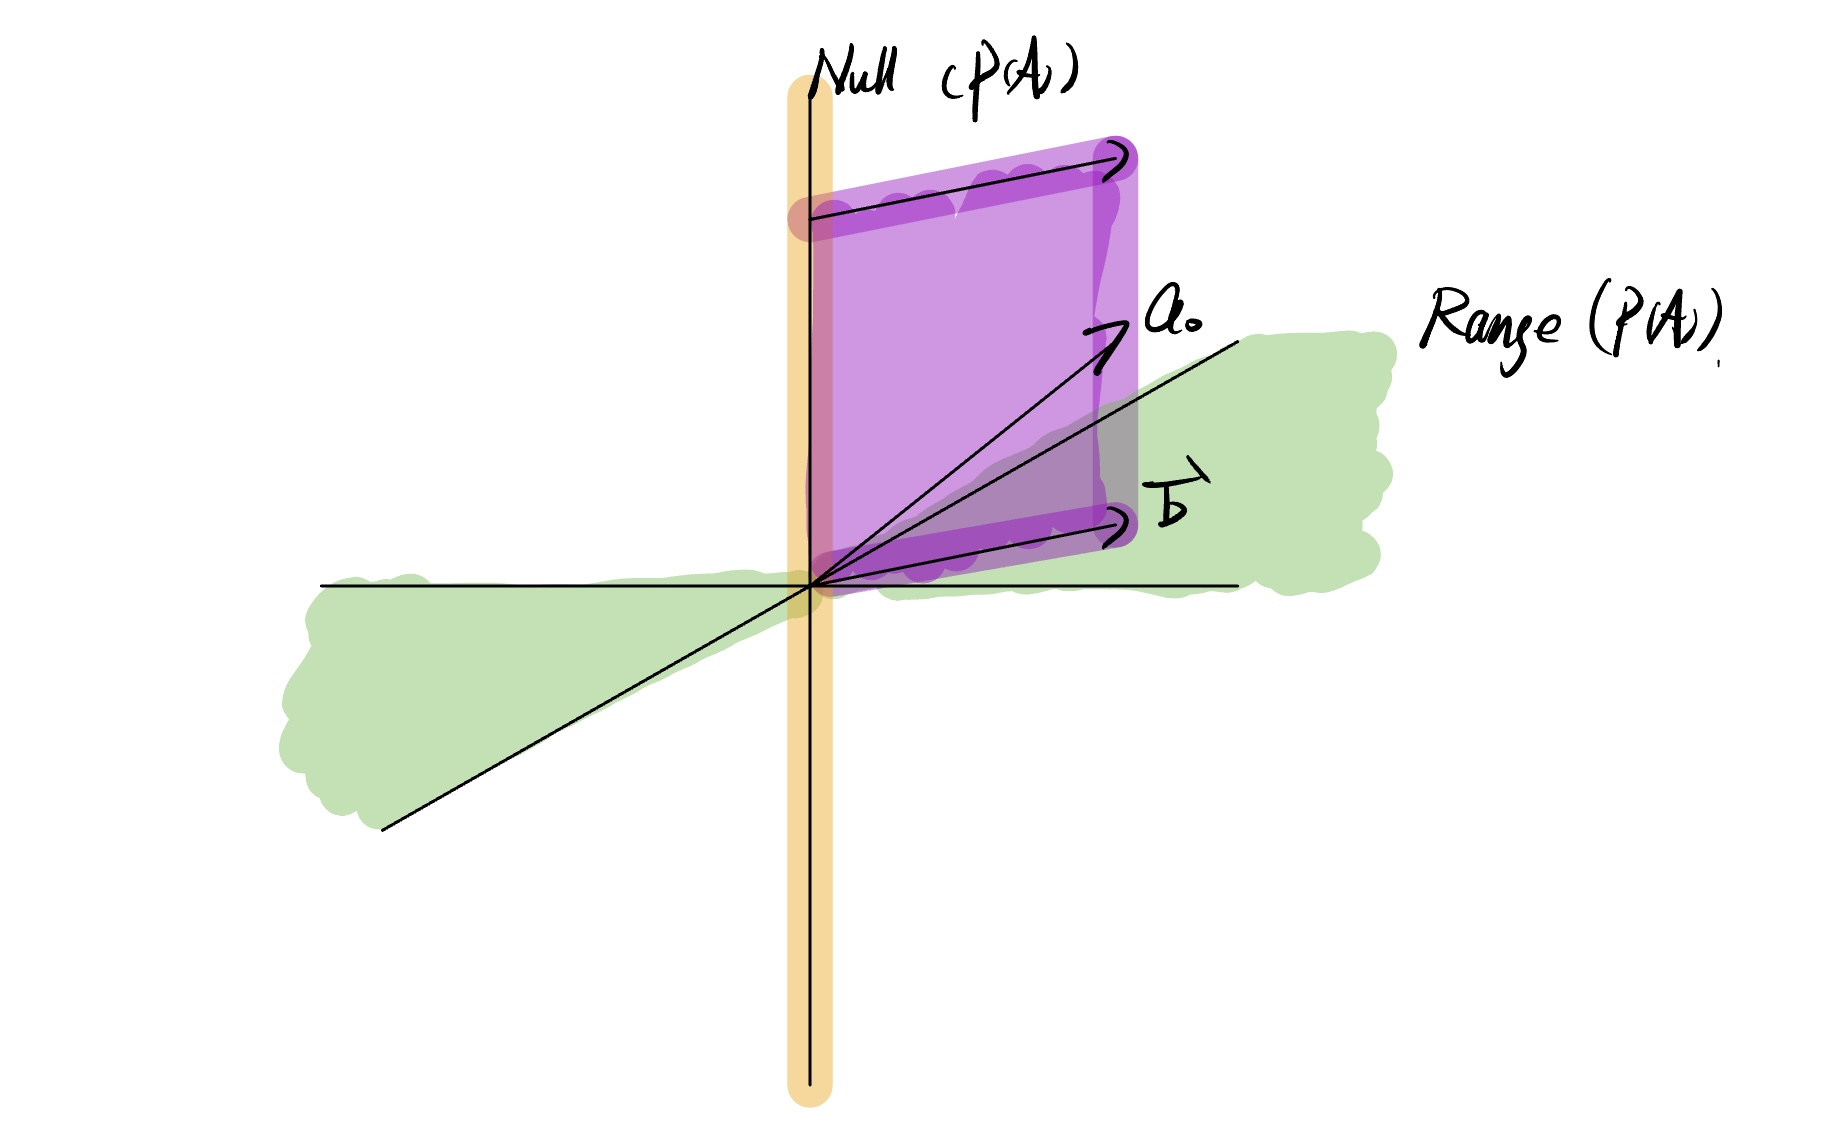
\includegraphics[scale=0.2]{Images/IMG_0291.jpg}
        \caption{My intuition}
    \end{figure}
\end{proof}

\noindent \textbf{Example}:
Solve the non-homogeneous equations.\\
\begin{enumerate}
    \item $a_{n+1}=2a_n+1$
    \item $a_{n+1}=2a_n+3^n$
\end{enumerate}

\noindent\textbf{Answer}:\\
\begin{enumerate}
    \item \begin{itemize}
        \item Let $A$ be the advancement operator. Then we have $$(A-2)\vec{a}=1$$ as the corresponding advancement polynomial equation.
        Let $p(A)=A-2$, first, let's compute $\vec{a_1} \in Null(p(A))$.
        $$(A-2)\vec{a}=0$$
        By the advancement theorem, $a_n=\alpha2^n$. This should be our $\vec{a_1}$.
        \item We only need to find a particular solution, this is usually the hard part.\\
        \underline{One way to do is trying to homogenize it.}
        \begin{equation}
            \begin{cases}
                a_{n+1}-2a_n=1\\
                a_{n+2}-2a_{n+1}=1
            \end{cases}
        \end{equation}
        We use the second equation to minus the first equation:
        $$a_{n+2}-3a_{n+1}+2a_n=0$$
        The corresponding advancement polynomial equation is
        $$(A^2-3A+2)\vec{a}=0$$ $$(A-1)(A-1)\vec{a}=0$$
        By the advancement theorem we have $$a_n=\alpha \cdot 2^n+\beta \cdot 1^n$$
        We notice that $\beta \cdot 1^n$ should be our particular solution $\vec{a_0}$. we should have 
        $$\beta=2\beta+1$$ $$\beta=-1$$
        Therefore, our solution is 
        $$a_n=\alpha \cdot 2^n-1$$
    \end{itemize}
    \item \begin{itemize}
        \item The first part is exactly as the last question, so we have $\vec{a_1}$ which is the sequence $\alpha \cdot 2^n$
        \item I will use two different methods to find the particular solution.
        \begin{enumerate}
            \item \underline{Guess then verify}: Try something that looks a lot like the right hand side.\\
            Guess: $\vec{a_0}$ is the sequence $d \cdot 3^n$.\\
            Solve the polynomial equation $$(A-2)\vec{a_0}=3^n$$ $$d \cdot 3^{n+1}-2 \cdot 3^n=3^n$$ $$3^n(3d-3)=0$$ $$d=1$$
            So $\vec{a_0}$ is the sequence $3^n$
            \item \underline{Trying to homogenize it}: Similar to the last question.\\
            \begin{equation}
                \begin{cases}
                    a_{n+1}-2a_n=3^n\\
                    a_{n+1}-2a_{n+1}=3^{n+1}
                \end{cases}
            \end{equation}
        \end{enumerate}
    \end{itemize}
\end{enumerate}


\section{Generating Functions and Recurrence}
The purpose of a generating function is using a function as a bookkeeping system for a sequence. And we can play the sequence in the continuous world. 
So what is the generating functions look like when we considering the advancement operator?

\begin{theorem}
    Assume the ordinary generating function for $\vec{a}$ is $$F(x)=\sum_{n=0}^{\infty}a_nx^n$$
    Then the ordinary generating function for $A\vec{a}$ is 
    \begin{equation}
        \begin{split}
            \sum_{n=0}^{\infty}a_{n+1}x^n &= \sum_{n=1}^{\infty}a_nx^{n-1}\\
            &= \frac{1}{x} \cdot \sum_{n=1}^{\infty}a_nx^n\\
            &= \frac{1}{x} \cdot (\sum_{n=0}^{\infty}a_nx^n -a_0x^0)\\
            &= \frac{1}{x} \cdot (F(x)-a_0)
        \end{split}
    \end{equation}
\end{theorem}

\begin{theorem}
    Assume the ordinary generating function for $\vec{a}$ is $$F(x)=\sum_{n=0}^{\infty}a_nx^n$$
    Then the ordinary generating function for $A^k\vec{a}$ is 
    \begin{equation}
        \begin{split}
            \sum_{n=0}^{\infty}a_{n+k}x^n &= \sum_{n=k}^{\infty}a_nx^{n-k}\\
            &= \frac{1}{x^k} \cdot \sum_{n=k}^{\infty}a_nx^n\\
            &= \frac{1}{x^k} \cdot (\sum_{n=0}^{\infty}a_nx^n -\sum_{n=0}^{k-1}a_nx^n)\\
            &= \frac{1}{x^k} \cdot (F(x)-\sum_{n=0}^{k-1}a_nx^n)
        \end{split}
    \end{equation}
\end{theorem}

\noindent \textbf{Example}: Suppose $a_n$ is a recurrence that satisfies the equation $$a_{n+3}=5a_{n+1}-a_n+3^n$$
Find a general form for it's ordinary generating function.

\noindent \textbf{Answer}:\\
\begin{equation}
    \begin{split}
        F(x) &= \sum_{n=0}^{\infty}a_nx^n\\
        &= a_0x^0+a_1x^1+a_2x^2+\sum_{n=3}^{\infty}a_nx^n\\
        &= a_0x^0+a_1x^1+a_2x^2+ x^3 (\sum_{n=0}^{\infty}a_{n+3}x^n)\\
        &= a_0x^0+a_1x^1+a_2x^2+ x^3 (5\sum_{n=0}^{\infty}a_{n+1}x^n -\sum_{n=0}^{\infty}a_{n}x^n +\sum_{n=0}^{\infty}3^nx^n)\\
        &= a_0x^0+a_1x^1+a_2x^2+ x^3 (\frac{5}{x}(F(x)-a_0) -F(x) + \frac{1}{1-3x})\\
    \end{split}
\end{equation}
Rearrange the equation above we get $$F(x)= \frac{a_0+a_1x+(a_2-5a_0)x^2}{1-5x^2+x^3} + \frac{x^3}{(1-5x^2+x^3)(1-3x)}$$

\begin{theorem}
    Assume the exponential generating function for $\vec{a}$ is $$f(x)=\sum_{n=0}^{\infty}a_n \frac{x^n}{n!}$$
    Then the exponential generating function for $A\vec{a}$ is $$\sum_{n=0}^{\infty}a_{n+1}\frac{x^n}{n!}=f'(x)$$
\end{theorem}

\noindent \textbf{Remark}:
\begin{itemize}
    \item For ordinary generating functions, we simply need to do algebra.
    \item For exponential generating functions, we need to solve differential equations. (harder!)
\end{itemize}

\noindent \textbf{Example}: Recall, the number of derangements $d_n$ satisfied the recurrence $$d_{n+1}=n \cdot d_n+n \cdot d_{n-1}$$
Find the general form of the exponential generating function $f(x)$ for $d_n$.

\noindent \textbf{Answer}:\\
By definition we have $$f(x)=\sum_{n=0}^{\infty}d_n\frac{x^n}{n!}$$
Consider the derivative of $f(x)$
\begin{equation}
    \begin{split}
        f'(x) &= \sum_{n=0}^{\infty}d_{n+1}\frac{x^n}{n!}\\
        &= \sum_{n=0}^{\infty}nd_n\frac{x^n}{n!}+ \sum_{n=0}^{\infty}nd_{n-1}\frac{x^n}{n!}\\
        &= x \sum_{n=1}^{\infty}d_n\frac{x^{n-1}}{(n-1)!} + x \sum_{n=1}^{\infty}d_{n-1}\frac{x^{n-1}}{(n-1)!}\\
        &= xf'(x)+xf(x)
    \end{split}
\end{equation}
The only thing we need to do is solving the ODE:\\
Rearrange the equation we have
$$(1-x)f'(x)=xf(x)$$ $$\frac{f'(x)}{f(x)}=\frac{x}{1-x}$$
Integrate both sides we have 
$$log(f(x))=-x-log(1-x)+c$$ $$f(x)=\frac{e^{-x+c}}{x-1}$$

\noindent \textbf{Example}\label{cnr}: Suppose $a_n$ satisfies $a_0=a_1=1$ 
and the Catalan recurrence $$a_{n+1}=\sum_{k=0}^{n}a_{n-k}a_k$$
Find the general form of the exponential generating function $F(x)$ for $a_n$.

\noindent \textbf{Answer}:\\
By definition we have $$F(x)=\sum_{n=0}^{\infty}a_n\frac{x^n}{n!}$$
Consider the square of $F(x)$
\begin{equation}
    \begin{split}
        F^2(x) &= \sum_{n=0}^{\infty}(\sum_{k=0}^na_ka_{n-k})x^n\\
        &= \sum_{n=0}^{\infty}a_{n+1}x^n\\
        &= \frac{1}{x} \cdot \sum_{n=0}^{\infty}a_{n+1}x^{n+1}\\
        &= \frac{1}{x} \cdot (\sum_{n=0}^{\infty}a_{n}x^{n} -a_0x^0)\\
        &= \frac{1}{x} \cdot (F(x)-1)
    \end{split}
\end{equation}
Rearrange the equation we have
$$xF^2(x)-F(x)+1=0$$
$$F(X)=\frac{1 \pm \sqrt{1-4x}}{2x}$$
Since $a_0=\lim_{x \to 0}F(x)$, hence we have 
$$F(X)=\frac{1 - \sqrt{1-4x}}{2x}$$
Can use Newton's binomial theorem to compute $$a_n=\frac{1}{n+1}{2n \choose n}$$
\chapter{Combinatorial Game Theory}


\section{Basic Terminologies}

\begin{definition}
    \textbf{Games of chance} are games with a randomness component. i.e. a people's decisions do not entirely dictate their outcomes.
\end{definition}
\textbf{Example}:Roulette in the casino.


\begin{definition}
    \textbf{Games of partial information} are games where a player is not privy to all available information when making a turn.(no simultaneous movement)
\end{definition}
\textbf{Example}:Poker: a player does not know the cards of other opponent.


\begin{definition}
    \textbf{Sequential games} are games where players alternate turns one after the other.
\end{definition}
\textbf{Example}:A mordern video game, say GTA5 online, is a non-sequential game that everyone can move simultaneously.


\begin{definition}
    \textbf{Games of perfect information} are games where both players have access to all available information.
\end{definition}


\begin{definition}
    \textbf{Well-founded games} are games where after a finite number of turns, the game ends.
\end{definition}
\textbf{Remark}:
\begin{itemize}
    \item Chess is not well-founded since players can moving pieces back and forth.
    \item Fun fact: Mathematically speaking, no well-founded game is fair.
\end{itemize}

\noindent \textbf{Note}:
\begin{itemize}
    \item Games of chance and games of partial information lie mostly in the realm of probability theory and economics.(research initialed by J.Von Neumman and J.Nash) 
    We will mostly be interested in games where both players have perfect information, and the game inevitably must end.(Sadly, this leaves chess out, though there is some research in this regard.)
    \item We also stick with two player games, though the theory of n-player games can be reduced to two players (Assuming all $n-1$ other players are colluding and form a second player)
\end{itemize}


\section{Three Simple Games}

\noindent \textbf{Tic-Tac-Toe}\\

\textbf{Introduction}:
\begin{itemize}
    \item Tic-Tac-Toe is a game between two players that takes place on a three by three grid.
    \item Players take turns filling in the grid one square at a time.
    \item The first player only fills the grid with X's.
    \item The second player only fills with O's.
    \item The game ends when a player has taken three positions that form a line in the grid.
\end{itemize}
\begin{figure}[ht]
    \centering
    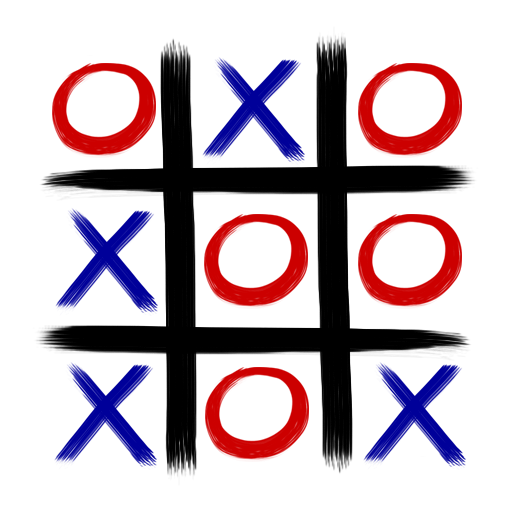
\includegraphics[scale=0.4]{Images/TicTacToe_HD_iTunesArtwork.png}
    \caption{A picture of tic-tac-toe}
\end{figure}

\textbf{Observation}:
\begin{itemize}
    \item It is a sequential game.
    \item The game is of perfect information.
    \item The game was played fast and well-founded.
    \item The first player was favoured.
    \item The game ties early.
    \item The only way that a player losses is if they make a mistake.
\end{itemize}


\noindent \textbf{Nim}\\

\textbf{Introduction}:
\begin{itemize}
    \item The set up is just three piles of stones. $(a,b,c)$ where each entry is apositive integer number of stones. $a,b,c \in \Z^+$
    \item Each turn, a player will pick a pile and remove any number of stones from that pile. For example, if it is player1's turn and the board state is $(5,2,0)$, then 
    $$(5,2,0) \longrightarrow (4,2,0)$$ $$(5,2,0) \longrightarrow (0,2,0)$$ $$(5,2,0) \longrightarrow (5,1,0)$$
    are all valid responses, but $(4,1,0)$ is not.
    \item The winning player is the one who drew the last stone.(Alternatively, the loser is the one with no stones to grab)
\end{itemize}
\begin{figure}[ht]
    \centering
    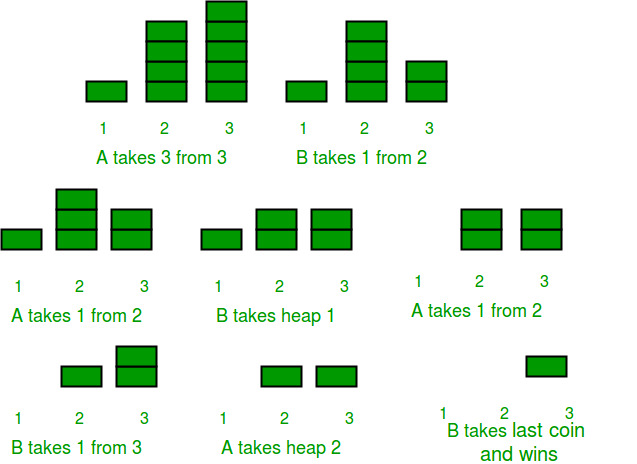
\includegraphics[scale=0.4]{Images/game3-2.jpeg}
    \caption{An example of Nim}
\end{figure}

\textbf{Observation}:
\begin{itemize}
    \item It is asequential game.
    \item The game is of perfect information.
    \item The game is well-founded and appears to be decided early.
    \item The nim depends on the initial pile.
    \item The first player seems to have advantage.
    \item The game is symmetric.
    \item The moment when we force two equal piles, the game is over.
    \item Nim always has a winner.
\end{itemize}


\noindent \textbf{The N-Gale-Stewart Game}\\

\textbf{Introduction}:
\begin{itemize}
    \item Let $A$ be a subset of length $N$ binary strings.
    \item Two players take turns picking either 0 or 1.
    \item The game terminates when the string hits length $N$.
    \item Player1(Alice) wins if the created string $s \in A$. Else, player2(Bob) wins.
\end{itemize}


\section{Formalizing Game}

\begin{definition}
    A \textbf{game} $\mathcal{G}$ between two players 1 and 2 is a collection of rules.
\end{definition}

\begin{definition}
    A \textbf{run/play} of the game is string of alternating moves $x_iy_i$ between player1 and player2.
\end{definition}

\begin{definition}
    Each player has a disjoint set $A_1$ and $A_2$ of terminal runs of the game called \textbf{payoff sets}.
\end{definition}

\begin{definition}
    We say player1 \textbf{wins a run} if and only if a run of the game $s \in A_1$ and similarly for player2.
\end{definition}
\textbf{Example}: For a Nim starts at the state $(3,4,4)$, for the game that we played in the class, we have a string 
$$(0,4,4) \cdot (0,2,4) \cdot (0,2,2) \cdot (0,0,2) \cdot (0,0,0)$$ This string would be inside player1's payoff set $A_1$.

\begin{definition}
    \textbf{Game states} are strings $s$ where $\forall i \in \N. s(2i-1)=x \text{ and } s(2i)=y_i$.
    We consider the empty string $\emptyset$ as the start of the game.
\end{definition}
\textbf{Remark}:
\begin{itemize}
    \item Sequence/string generally are interchangeable in mathematics, but we stick with the notion of string as they're finite most of the time and we don't want to mix-up/confuse you with sequences from analysis (which on the flipside are almost always presumed to be infinite).
    \item Game state refers to the strings s, places the game COULD go. Run usually is reserved for terminal game states i.e the strings t where the game has ended. 
\end{itemize}

\begin{definition}
    We call a game $\mathcal{G}$ \textbf{well-founded} if every possible run of the game ends after finitely many turns. We say it is \textbf{ill-founded} if it is not well-founded.
\end{definition}

\begin{definition}
    Given a game $\mathcal{G}$, \textbf{the game tree} $T_{\mathcal{G}}$ is the poset of all possible game states. We say $s \leq_{\mathcal{G}} t$ if for all $i$ in the domain of $s$, $s(i)=s(t)$. 
    When we dipict the game tree, we always mean the cover graph of $T_{\mathcal{G}}$ (Note, the cover graph will always be a tree, hence the name)
\end{definition}
\begin{figure}[ht]
    \centering
    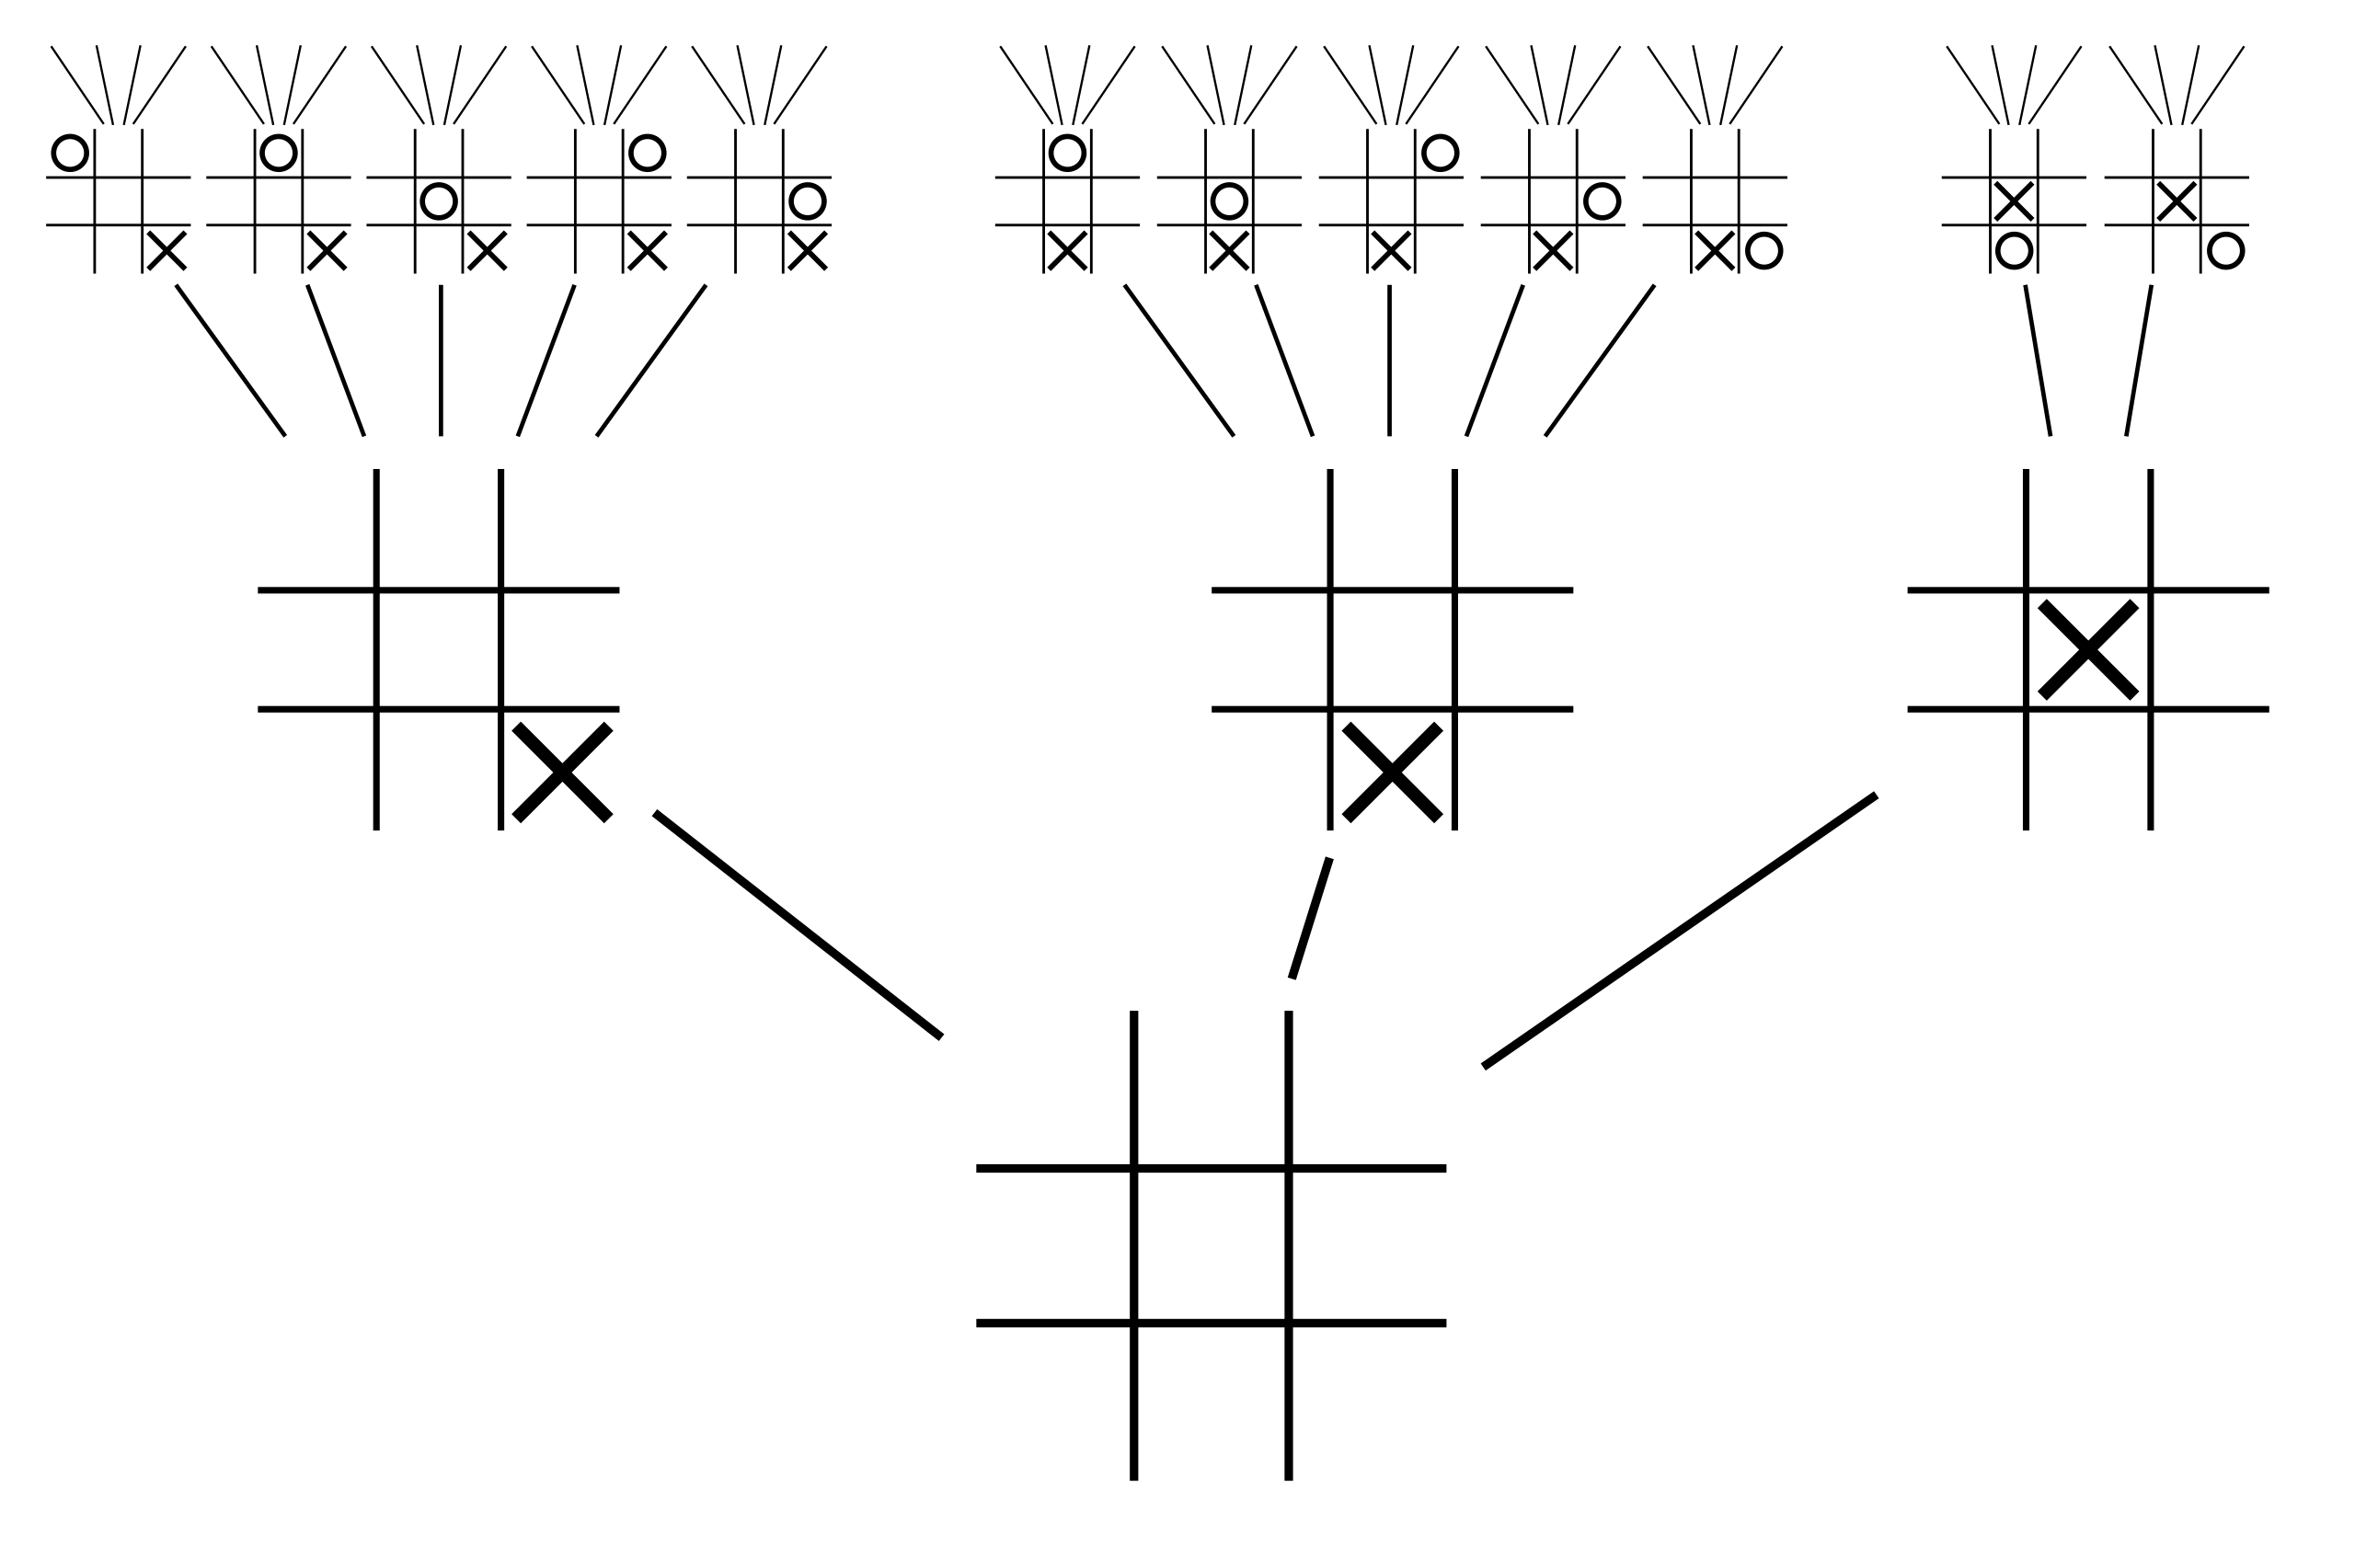
\includegraphics[scale=0.1]{Images/Tic-tac-toe-game-tree.svg.png}
    \caption{Incomplete game tree of tic-tac-toe}
\end{figure}





\section{Strateries for Games}

\noindent \textbf{What is strategy?}
\begin{itemize}
    \item A colletion of responses to a particular outcome.
    \item A response to acurrent game state that gets close to a payoff state.
\end{itemize}

\begin{definition}
    Let $\mathcal{G}$ be a game between Alice and Bob.(Alice goes first). 
    A \textbf{strategy} for Alice is a function $f$ that takes game state $s$ of length $2n$ and returns a game state $f(s)$.
    $$f:s \longrightarrow f(s)$$
    where $length(f(s))=2n+1$ and $s \leq_{\mathcal{G}} f(s)$.i.e. it provides a response to any move Bob can make in any situation.
\end{definition}
\textbf{Remark}:
\begin{itemize}
    \item A strategy for Bob is defined symmetrically.
\end{itemize}

\textbf{Example}:
\begin{itemize}
    \item \textbf{The mirroring strategy} for Bob is playing whatever Alice played.
    \item \textbf{The zero strategy} for Bob is always picking zero.
\end{itemize}

\begin{definition}
    Given a game $\mathcal{G}$, we call a strategy \textbf{winning} if whether the player uses it, he win.
\end{definition}
\textbf{Example}:
Consider the 4-Gale-Stewart game with payoff set $A=\{0101,0001,0100,0000\}$
\begin{itemize}
    \item The zero strategy for Alice is winning.
    \item The mirroring strategy for Bob is not winning.
\end{itemize}

\begin{theorem}[The first strategy theorem]
    Given a game $\mathcal{G}$, both Alice and Bob cannot have a winning strategy.
\end{theorem}
\begin{proof}
    Let $f$ be the winning strategy of Alice, and let $g$ be the winning strategy of Bob. 
    Play a run of the game where Alice plays according to $f$ and Boo plays according to $g$. 
    Since $f$ is winning, Alice wins. Since $g$ is winning, Bob wins. 
    This is a contradiction, games can only hane one winner.
\end{proof}

\begin{definition}
    Given an integer $n$, it's associated \textbf{binary representation} is the unique sequence $a_k \in \{0,1\}$ (from right to left) with the property that $$n=\sum_{k=0}^na_k\cdot 2^k$$
\end{definition}

\begin{definition}
    Given two binary strings $s$ and $t$, the \textbf{nim-sum} $$s \oplus t$$ 
    is the binary string $r$ where $$r(i)=0 \text{ iff } s(i)=t(i)$$
\end{definition}
\textbf{Example}:
\begin{itemize}
    \item $111 \oplus 101=010=10$
    \item $1110000 \oplus 1111 = 1110000 \oplus 0001111=1111111$
    \item $10101 \oplus 10101=000000=0$
\end{itemize}

\begin{theorem}[Properties of nim-sum]\
    \begin{itemize}
        \item $s \oplus t = t \oplus s$
        \item $(s \oplus t) \oplus r = s \oplus (r \oplus t)$
        \item $s \oplus 0=s$
        \item $s \oplus t =0 \text{ iff } s=t$
    \end{itemize}
\end{theorem}
\textbf{Remark}:
\begin{itemize}
    \item Let $\{0,1\}^+$ denotes $\{0,1\}^*-\{\lambda\}$. 
    Let $\forall x \in \{0,1\}^+.i(x)=x$\\
    Then $(\{0,1\}^+, \oplus, 0, i)$ is a group, futher, am abelian group.
    \item From the algebraic perspective, the last property means that in this abelian group, the inverse of x is x itself.
    \item The essense of nim-sum:
    \item \begin{itemize}
        \item if the nim-sum of two piles equals zero, then the two piles have the same amount of stones.
        \item if the nim-sum of three piles equals zero, then the amount of stones in the largest pile equals to the sum of stones in the other two smaller piles.
    \end{itemize}
\end{itemize}

Informally, we can define an \textbf{equilibrium state} when the amount of stones in the largest pile equals the amount of stones in the other two piles.\\

If we played the game some times, we will notice:
\begin{itemize}
    \item if we are at an equilibrium state, then whatever we do, the next state is not equilibrium.
    \item if we are at a non-equilibrium state, then we can do something to make the next state equilibrium.
\end{itemize}
We can formalize our observation to make the following lemmas.

\begin{lemma}
    Suppose in a game of Nim, the piles have $s_1,s_2,s_3$ many stones where the number is written in binary. 
    If $s_1 \oplus s_2 \oplus s_3=0$, then after any move to the board state $t_1,t_2,t_3$, we have $t_1 \oplus t_2 \oplus t_3 \neq 0$
\end{lemma}
\begin{proof}
    Suppose $s_1 \oplus s_2 \oplus s_3=0$. 
    Suppose without loss of generality, we remove some number from the first pile $s_1$. 
    So the board state is now $t_1,s_2,s_3$. 
    We claim that there is a non-zero $r$ such that $s_1=t_1 \oplus r$. 
    (if $r=0$, then $t_1=s_1$ and we removed nothing) 
    By way of contradiction, suppose $t_1 \oplus s_2 \oplus s_3=0$.
    It follows that 
    \begin{equation}
        \begin{split}
            s_1 \oplus s_2 \oplus s_3 &= (r \oplus t_1) \oplus s_2 \oplus s_3\\
            &= r \oplus (t_1 \oplus s_2 \oplus s_3)\\
            &= r \oplus 0\\
            &= 0
        \end{split}
    \end{equation}
    Hence $r=0$, this is a contradiction.
\end{proof}



\begin{lemma}
    Suppose $s_1,s_2$ and $s_3$ is the current board state in a game of Nim, and $$s_1 \oplus s_2 \oplus s_3 \neq 0$$
    Then there is a move that can be made to the board state $t_1,t_2,t_3$ such that $$t_1 \oplus t_2 \oplus t_3=0$$
\end{lemma}
\begin{proof}
    Since $s_1 \oplus s_2 \oplus s_3$ is non-zero binary string. 
    Then the string $s_1 \oplus s_2 \oplus s_3$ has a leading 1. 
    Assume the leading 1 is at the i-th spot from right to left. 
    It follows that one of one of $s_1,s_2,s_3$ has a 1 in the i-th spot. 
    (either 3 of them have ones or just one of them has a one in the i-th spot)
    Without loss of generality, suppose it is $s_1$. We claim that $s_1 \oplus (s_1 \oplus s_2 \oplus s_3)$ is less than $s_1$.
    \begin{equation}
        \begin{split}
            s_1 \oplus (s_1 \oplus s_2 \oplus s_3) &= (s_1 \oplus s_1) \oplus s_2 \oplus s_3\\
            &= 0 \oplus s_2 \oplus s_3\\
            &= s_2 \oplus s_3
        \end{split}
    \end{equation}
    By assumption, all spots on the left side of the i-th spot of $s_2 \oplus s_3$ must be the same as the corresponding spots of $s_1$. 
    For the i-th spot, $s(i)=1$ and $s_2 \oplus s_3(i)=0$. It suffices to conclude that $s_2 \oplus s_3 <s_1$.
    Remove blocks from $s_1$, make $t_1=s_1 \oplus (s_1 \oplus s_2 \oplus s_3)=s_2 \oplus s_3$. 
    It follows that the nim-sum of the three piles is now 
    \begin{equation}
        \begin{split}
            t_1 \oplus s_s \oplus s_3 &= (s_2 \oplus s_3) \oplus s_2 \oplus s_3\\
            &= (s_2 \oplus s_3) \oplus (s_2 \oplus s_3)\\
            &= 0
        \end{split}
    \end{equation}
\end{proof}


\begin{theorem}[Winning strategy for Nim]
    Let $s_1,s_2$ and $s_3$ be the starting board state of a game of Nim. 
    If $s_1 \oplus s_2 \oplus s_3 \neq 0$, then the player1(Alice) has a winning strategy. Else, player2(Bob) has a winning strategy.
\end{theorem}
\begin{proof}
    Suppose $s_1 \oplus s_2 \oplus s_3 \neq 0$. 
    Let Alice play with the strategy that she always moves so that the following board state satisfies $t_1 \oplus t_2 \oplus t_3 =0$. 
    By the second lemma, such a move is always possible. By the first lemma, no matter what move Bob makes, the nim-sum will be non-zero(hence we can make the nim-sum zero) 
    Since the total number of stones is finite and it decreases each turn. Hence the game must terminate. 
    Note, when it ends, the nim-sum of the piles must be zero. 
    Hence it was Alice that made the last move and she wins. 
    If $s_1 \oplus s_2 \oplus s_3=0$, any move Alice makes will make the nim-sum of thr pile non-zero. 
    Bob then canplay with Alice's strategy which symmetically is winning.
\end{proof}


\section{Determinism}


\begin{definition}
    we say a game $\mathcal{G}$ is \textbf{determined} if one of the players has a winning strategy.
\end{definition}
\textbf{Remark}:
\begin{itemize}
    \item We now know Nim is determined.
\end{itemize}

\begin{theorem}[N-Gale-Stewart is determined]
    For every subset of length $N$ binary strings $A$, the N-Gale-Stewart game where Alice has payoff set $A$ is determined.
\end{theorem}
\begin{proof}
    By induction on $N \in\N$\\
    Base case: The only strings of length 1 are 0 and 1.
    \begin{itemize}
        \item If $A \neq \emptyset$, then Alice has a winning strategy since she can simply choose 1 or 0 depending on which is in $A$.
        \item If $A = \emptyset$, then Bob has a winning strategy since no matter what move Alice makes, doing nothing can win.
    \end{itemize}
    Inductive step: Suppose the N-Gale-Stewart game is determined for any payoff set. 
    Consider an (N+1)-Gale-Stewart game. Let $A$ be the payoff set for Alice. Let $A'$ be the set of $N$ length binary strings defined by:
    \begin{itemize}
        \item For all $x \in A$, we have a prefix of $X$ with lengh $N$.
        \item We call this prefix $p$ and we put $p$ in the set $A'$.
    \end{itemize}
    \begin{figure}[ht]
        \centering
        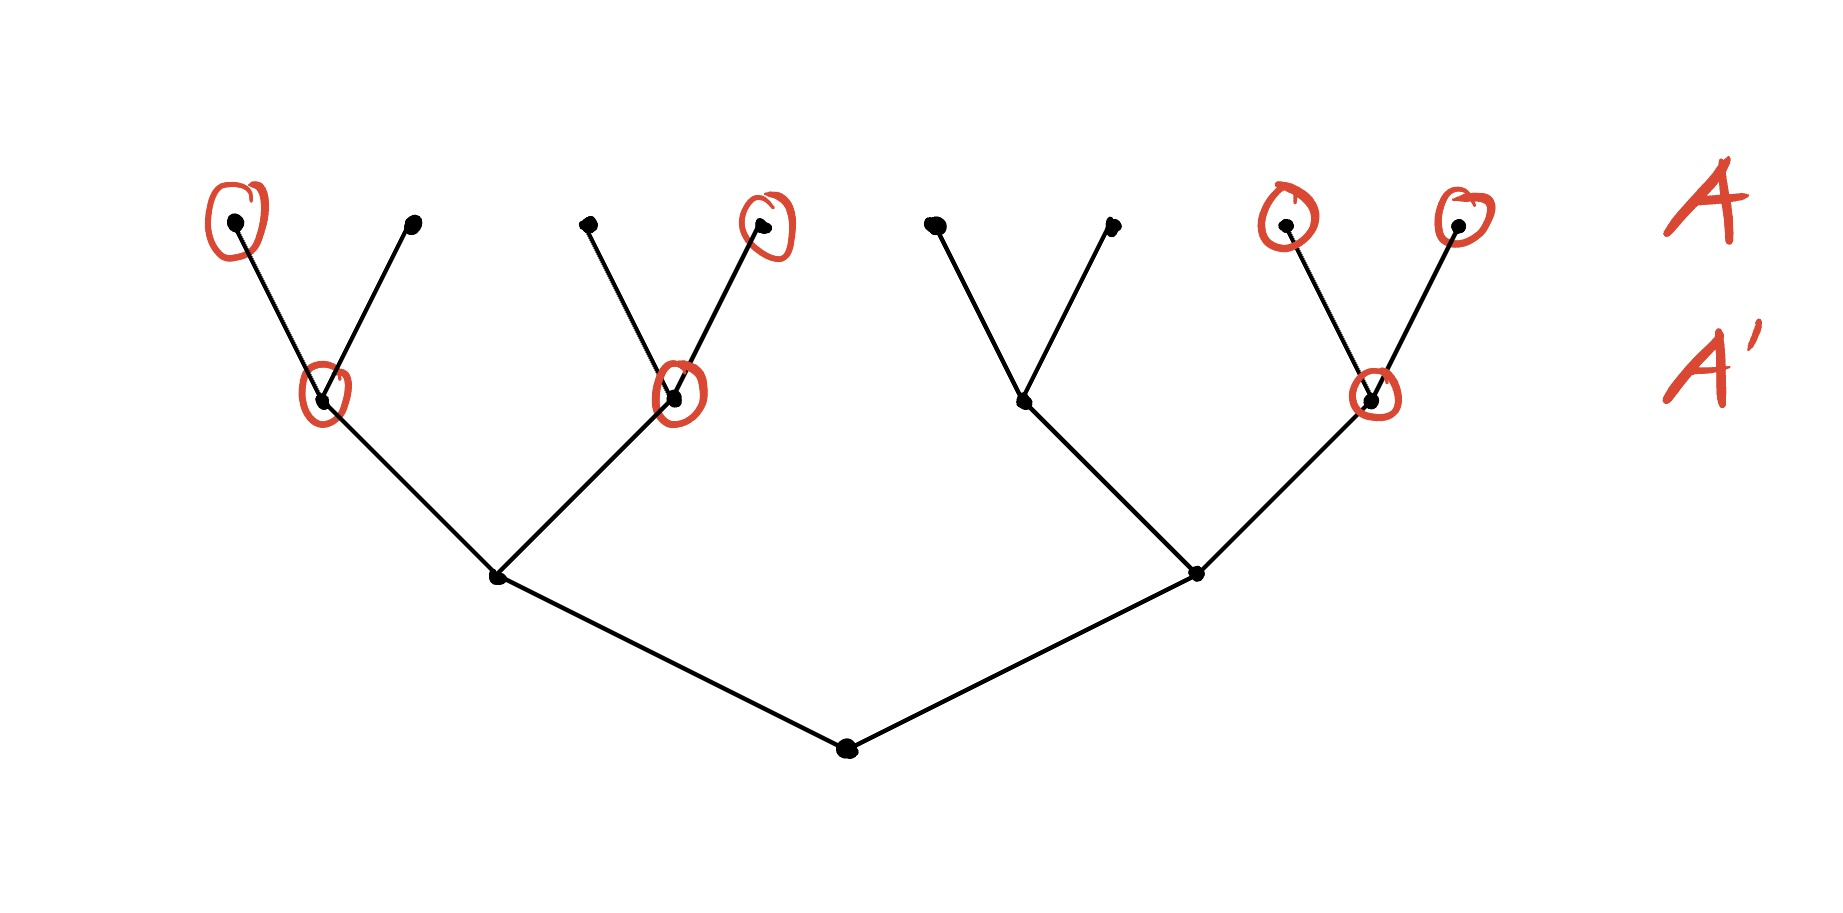
\includegraphics[scale=0.15]{Images/IMG_0295.jpg}
        \caption{An example of definining $A'$}
    \end{figure}
    So by our definition, any $p \in A'$ is $\leq_{\mathcal{G}}$-below some string in $A$.
    Now we can define a subgame: A N-Gale-Stewart game with payoff set for Alice $A'$. 
    By the induction hypothesis. This subgame is determined. 
    Hence one of Alice and Bob has the winning strategy. Without loss of generality, assume Alice makes the last move for the (N+1)-Gale-Stewart game. 
    Hence Bob makes the last move for the subgame. 
    \begin{itemize}
        \item If the winning strategy for the N-Gale-Stewart subgame is for Alice and she using that strategy during the game. Hence whatever the letter Bob choose, the string $p$ the make, is in $A'$. Then Alice can choose the last digit of the corresponding $X$ in $A$. 
        Therefore, Alice has a winning strategy a winning strategy for the (N+1)-Gale-Stewart game.
        \item If the winning strategy for the N-Gale-Stewart subgame is for Bob and he using that strategy during the game. Hence the string $p$ they make, is in $\{0,1\}^N-A'$. So whatever letter that Alice choose, the string $x$ they make is in $\{0,1\}^{N+1}-A$. Hence Bob wins. 
        Therefore, Bob has a winning strategy for the (N+1)-Gale-Stewart game.
    \end{itemize}
\end{proof}
\textbf{Remark}:
\begin{itemize}
    \item The strategy is sometimes called \underline{backtracking}, as we've trying to reverse a win from terminal game states.
\end{itemize}

\begin{theorem}[Zermelo's Theorem]
    Let $\mathcal{G}$ be a game with a well-founded game tree. Suppose every run of the game ends in a winner.(i.e. ties are not possible) Then a player has a winning strategy.
\end{theorem}
\begin{proof}
    Assume the game is finite. 
    We are going to apply the backtracking algorithm recursively.
    \begin{itemize}
        \item Start with the strings with the largest length. Colour them blue if Alice wins and red if Bob wins.
        \item Move down to the previous length strings. Without loss of generality, suppose it is Alice's turn. Colour the string blue if Alice can move to a blue string and red if all moves are red. (This step is symmetric for Bob)
    \end{itemize}
    Eventually, the empty string $\emptyset$ will be coloured. We claim that:
    \begin{itemize}
        \item If the colour is blue, then Alice has a winning strategy.
        \item If the colour is red, then Bob has a winning strategy.
    \end{itemize}
    Without loss of generality, suppose $\emptyset$ is blue. Alice will apply the strategy cotinuously:
    \begin{itemize}
        \item Alice can then choose a move to a game state coloured blue. Alice will play with the strategy of pickinga blue game state.
        \item Given Alice has chosen a game state that is coloured blue. On Bob's turn, it must be the case that all Bob's moves lead to game states that are coloured blue.
    \end{itemize}
    The game must terminate. When it does, Alice's strategy garantees the terminal state is blue. 
    By way we coloured the tree, a blue terminal game state means Alice wins.
\end{proof}

\begin{theorem}[Zermelo's Full Theorem]
    Let $\mathcal{G}$ be a game with a well-founded game tree, Then either the game is determined, or both players have strategies that either sin or force a tie.
\end{theorem}
\begin{proof}
    Consider the new games $\mathcal{G}_A$ and $\mathcal{G}_B$.
    \begin{itemize}
        \item $\mathcal{G}_A$ is played the same way as $\mathcal{G}$, but Alice wins as long as we do not reach Bob's payoff set.(i.e. if tiedin $\mathcal{G}$, then Alice wins)
        \item $\mathcal{G}_B$ is defined symmetrically.
    \end{itemize}
    Neither $\mathcal{G}_A$ nor $\mathcal{G}_B$ have ties, by the last theorem, they are determined.
    \begin{itemize}
        \item If $\mathcal{G}_A$ is determined in favour of Bob, then the strategy for Bob in this game is winning in $\mathcal{G}$.
        \item If $\mathcal{G}_B$ is determined in favour of Alice, then the strategy for Alice is winning in $\mathcal{G}$.
        \item Suppose Alice has a winning strategy in $\mathcal{G}_A$ and Bob has a winning strategy in $\mathcal{G}_B$. Then playing with Alice's strategy in $\mathcal{G}_A$ means BOb cannot win. similarly for Bob's. Hence, playing the strategies against one another in $\mathcal{G}$ forces a tie.
    \end{itemize}
\end{proof}
\textbf{Remark}:
\begin{itemize}
    \item Very naively, this suggests every well-founded game is in one of two forms. 
    A game like Nim which is favoured for somebody, or a game like tic-tac-toe where two perfect players always force a tie.
\end{itemize}

\noindent \textbf{Some words beyond}:\\
Consider the game Go:
\begin{itemize}
    \item The usual board is a 19 by 19 square with players either placing black or white pieces on the board.
    \item By our definition, the game Go is of perfect information and well-founded.
    \item By the Zermelo's full theorem: either Alice or Bob has a winning strategy, or two perfect player will end in a draw.
    \item Therefore, for any player that goes first in Go, he has a strategy that never lose theoretically.
\end{itemize}
Unfortunately, although the prof of Zermelo's theorem is constructive, the construction process requires us to get the whole game tree first. 
But in a game like Go, the number of terminal states is more than the number of atoms in the universe. It is impossible for now to get such strategy using this theorem.



\section{Infinite Games}

\begin{definition}
    A game is \textbf{ill-founded} if there are infinite runs.
\end{definition}
\textbf{Remark}:
\begin{itemize}
    \item Infinite runs tend to be the feature of infinite games, making our tools like Zermelo's theorem and methods like backtracking futile.
\end{itemize}


\begin{definition}
    The \textbf{Gale-Stewart game} is played as follows:
    \begin{itemize}
        \item Alice has some payoff set $A$ of infinite binary strings $s:\N \longrightarrow \{0,1\}$.
        \item Alice and Bob take turns choosing either 0 or 1.
        \item Alice wins if the created string is in $A$ and Bob wins otherwise.
    \end{itemize}
\end{definition}

\begin{lemma}
    If the payoff set $A$ for Alice is finite in the Gale-Stewart game, then Bob has a winning strategy.
\end{lemma}
\begin{proof}
    Suppose $A=\{s_1,s_2.\cdots,s_k\}$. Bob will play with the strategy that on his i-th turn, he will pick 0 if $s_i(2i)=1$ and pick 1 otherwise. 
    On the rest of Bob's turn after his k-th turn, he will only pick 0. 
    Bob's strategy ensures that the terminal sequence $s$ satisfies the condition $s(2i) \neq s_i(2i)$ and hence $s \notin A$.
\end{proof}
\textbf{Remark}:
\begin{itemize}
    \item This is like the diagonalization proof.
    \item We can generalize the lemma to the situation that $A$ is countable.
\end{itemize}


\begin{theorem}[*]
    There is a set of binary string $A$ such that neither Alice nor Bob has a winning strategy in the Gale-Stewart game with payoff set $A$ for Alice.
\end{theorem}


\begin{definition}
    The \textbf{Kubis' Game(for Graphs)} is defined as follows:
    \begin{itemize}
        \item The game is between Alice and Bob.
        \item The game starts with the emptygraph $(\emptyset, \emptyset)$.
        \item On each player's turn, if the current graph is $(V,E)$, the player responds by adding new vertices $X$ and edges strictly between vertices in $X$ and $X \cup V$.(i.e. a player cannot add edges where there weren't any previously)
        \item Say Alice wins for a graph $K$ if in a run she can create a graph isomorphic to $K$.
    \end{itemize}
\end{definition}


\begin{lemma}
    If there us a graph $K$ for which Alice has a winning strategy, it must contain every finite graph as a subgraph.
\end{lemma}
\begin{proof}
    Fix a graph $G$. Let Alice play with her strategy. 
    Let Bob play with the strategy that on his turn, he always adds a disjoint copy of G. 
    Since Alice's strategy is winning, the final graph will be isomorphic to $K$. 
    By Bob's strategy, the graph will have infinitely many disjoint copies pf $G$ as a subgraph. 
    Since $G$ was arbitrary, this is true for any finite graph $G$.
\end{proof}

\begin{theorem}[*Erdos-Rado]
    There is an infinite graph $R=(V,E)$ which can be expressed as an $\N$ indexed union of finite graphs with the property that for every pair of finite disjoint vertex set $V_1$ and $V_2$, 
    there is a $v \in V$ which is adjacent to everything in $V_1$ and nothing in $V_2$. 
    Moreover, any infinite graph with this property is unique up to isomorphism.
\end{theorem}


\begin{theorem}
    There is a winning strategy for Alice for $R$ in the Kubis' game.
\end{theorem}
\begin{proof}
    Let Alice play with the strategy that on her turn, if the current graph is $(V,E)$, for any subset $A \subset V$, 
    she responds by adding vertex $v_A$ such that $v_A$ is connected to everything in $A$ and not connected to anything outside of $A$. 
    Suppose at the end of the game, we have an infinite graph $R$. 
    Take arbitrary subsets of vertices $V_1$ and $V_2$ such that $V_1.V_2$ disjoint. 
    At some stage of the game, all the vertices of $V_1$ and $V_2$ just appeared. 
    Shortly after, on Alice's turn, she added a vertex who's neighbours were $V_1$ and shared no edges with $V_2$. 
    It follows that this graph is isomorphic to $R$>
\end{proof}

\end{document}